\documentclass[scheme = chinese]{ctexart}

% Set page size and margins
% Replace `letterpaper' with`a4paper' for UK/EU standard size
\usepackage[a4paper,top=2cm,bottom=2cm,left=3cm,right=3cm,marginparwidth=1.75cm]{geometry}
% Useful packages
% \usepackage{amsmath}
\usepackage{graphicx}
\usepackage[colorlinks=false, allcolors=blue]{hyperref}
\usepackage[final]{pdfpages}
\usepackage{booktabs}
\usepackage{caption}
\usepackage{makecell}
\graphicspath{ {./images/} }
\usepackage{varioref}
\usepackage{float}
\usepackage{listings}
\usepackage{minted}
\usepackage{longtable}
\usepackage{subfiles}
\usepackage[figuresright]{rotating}
\usepackage[graphicx]{realboxes}
\usepackage{adjustbox}
\usepackage{blindtext}
\usepackage{listings}
\usepackage{color}
\usepackage{thmtools}
\usepackage[center]{titlesec}
\usepackage{amssymb}
\usepackage{enumitem}
\usepackage{outlines}

\hypersetup{
    colorlinks=true,
    linkcolor=black
}

\newcommand{\xor}[0]{\oplus}
\newcommand{\dott}[0]{^\bullet}

% \usepackage{amsthm}
% \usepackage{mathtools}
% \usepackage{float}
\usepackage[math-style=TeX]{unicode-math}
\usepackage{algorithm}
\usepackage{algorithmicx}
\usepackage{algpseudocode}
\usepackage{mathtools}
\DeclarePairedDelimiter\ceil{\lceil}{\rceil}

\renewcommand{\algorithmicrequire}{\textbf{Input:}}
\renewcommand{\algorithmicensure}{\textbf{Output:}}
\newcommand{\todo}[1]{{\Huge \color{red} #1}}

\setlist{leftmargin=4\ccwd}
\begin{document}

% latex封面
\begin{titlepage}
    \centering
    \rule{\textwidth}{0pt}
    \vspace{0.3\textheight}
    
    {\zihao{2} \heiti\sffamily 面向英文数据的编辑与信息检索系统}
    
    \vspace{0.2\textheight}
    {
        \zihao{4}\selectfont \songti
        学~~~~~~号 \underline{\qquad\;19071110\;\qquad} \\
        姓~~~~~~名 \underline{\qquad~~孙天天~~\qquad} \\ 
        指导教师   \underline{\qquad~~杜永萍~~\qquad} \\
    }
    \vfill
    
    {\fontsize{10.5pt}{10.5pt}\selectfont \songti \today}
    
    \vspace{0.25\textheight}
\end{titlepage}

% 设置
\title{数据结构课设报告}
\author{孙天天 19071110}

\ctexset{
    section = {
        titleformat = \centering\heiti\zihao{3},
        name = {,},
        aftertitle = \hspace{12pt},
    },
    subsection = {
        titleformat = \raggedright\heiti\zihao{4},
        name = {,},
        aftertitle = \hspace{6pt},
        indent = 2\ccwd
    },
    subsubsection = {
        titleformat = \raggedright\heiti\zihao{-4},
        name = {,},
        aftertitle = \hspace{3pt},
        indent = 2\ccwd
    },
    paragraph = {
        indent = 2\ccwd
    },
    subparagraph = {
        indent = 2\ccwd,
    },
    today = small,
    figurename = 图,
    contentsname = 目录,
    tablename = 表,
}
 
\titleformat*{\section}{\zihao{3}\setlength{\baselineskip}{12pt} \selectfont\heiti\sffamily \centering}
\titleformat*{\subsection}{\zihao{4}\setlength{\baselineskip}{6pt} \selectfont\heiti\sffamily}
\titleformat*{\subsubsection}{\zihao{-4}\setlength{\baselineskip}{3pt} \selectfont\heiti\sffamily}
\zihao{5} \songti

% 目录
\tableofcontents
\clearpage

\section{需求分析}
\subsection{题目需求描述}
题目要求文档中已经对需求进行了全面清晰的描述,这里结合我具体实现拓展要求的情况,对需求进行明确。

\subsubsection{文件管理功能}
基本要求中:对文件的创建、打开、保存功能。

我增加了:递归打开指定目录下所有文件、文件目录树状显示、显示未保存文件的功能。

\subsubsection{文本编辑功能}
基本需求中:文件内容编辑、单文件查找和替换的功能。

我增加了:在文本中自动选中搜索或替换结果、类似迭代器逐个替换、批量替换全部的功能。

\subsubsection{编码译码功能}
基本需求中:给定的文章片段按字频哈夫曼编码和译码,并图形化界面演示。

扩展要求中:对编码与译码的过程可以自行设计其他算法。对此我完成了哈夫曼编码译码和base64编码译码。

此外,我增加了:可视化编码中生成的哈夫曼树。

\subsubsection{词频统计功能}
基本要求中:对多篇文档统计词汇出现频率,排序并显示前30。

我增加了:每个词汇按文档分类,显示文档中词汇出现的每个位置,点击跳转到词汇出现的位置,自定义显示数量。

\subsubsection{高级检索功能}
基本要求中:对多篇文档检索关键词,显示检索结果。

扩展要求中:支持检索表达式,对检索结果按相关性排序(这点我使用TFIDF为权重实现)。

我增加了:根据同义词数据库联系同义词一起检索,点击跳转到词汇出现位置,自定义显示数量。

\subsection{选用的技术栈}
\subsubsection{从课设的角度} 本课设的重点在于练习数据结构和算法的设计、开发能力,这点对于大部分编程语言均可实现。而其图形化界面的展示功能不是课设的重点,为此应该选择可以高效快速构建图形化界面的技术栈。

这促使我想到了web前端技术栈,而考虑到前端开发通常可以使用组件库提高开发效率,我采用了前端框架Vue和组件库Ant Design of Vue。

\subsubsection{从产品的角度}
若将本课设看作一个小规模的产品,分析可能真正使用它的需求。我想对于这样轻量级的工具,快速启动和随开随用十分关键。

选用web前端技术栈进行开发,可以将其部署在静态web服务器上,用户打开网页即可使用,同时也不会占有过多服务器资源。

\subsubsection{使用的技术栈}
本课设使用web前端技术栈开发,具体如下:
\begin{itemize}
    \item 用户界面框架:Vue
    \item 网页结构:HTML
    \item 样式表:CSS、LESS
    \item 组件库:Ant Design of Vue
    \item 页面控制与动态反馈:JavaScript
    \item 数据结构与算法:JavaScript
\end{itemize}

\subsection{原型设计}
为了更准确地确定需求,我在开发之前进行了原型设计,绘制出了大致的图形界面效果,并说明其中的功能、用到的算法和数据结构。完成后我有老师就原型进行了讨论交流,确定了开发需求。

后来,在进行开发实践后,又对其中与实际不符的地方进行了简单修改。因此以下展示的原型功能与最终版本基本一致,但界面显示效果略有不同。

原型左侧为图形化界面的展示,右侧为对应的功能、实现的需求和用到的算法。其中黑色字为必须完成内容,深蓝色为拓展内容。

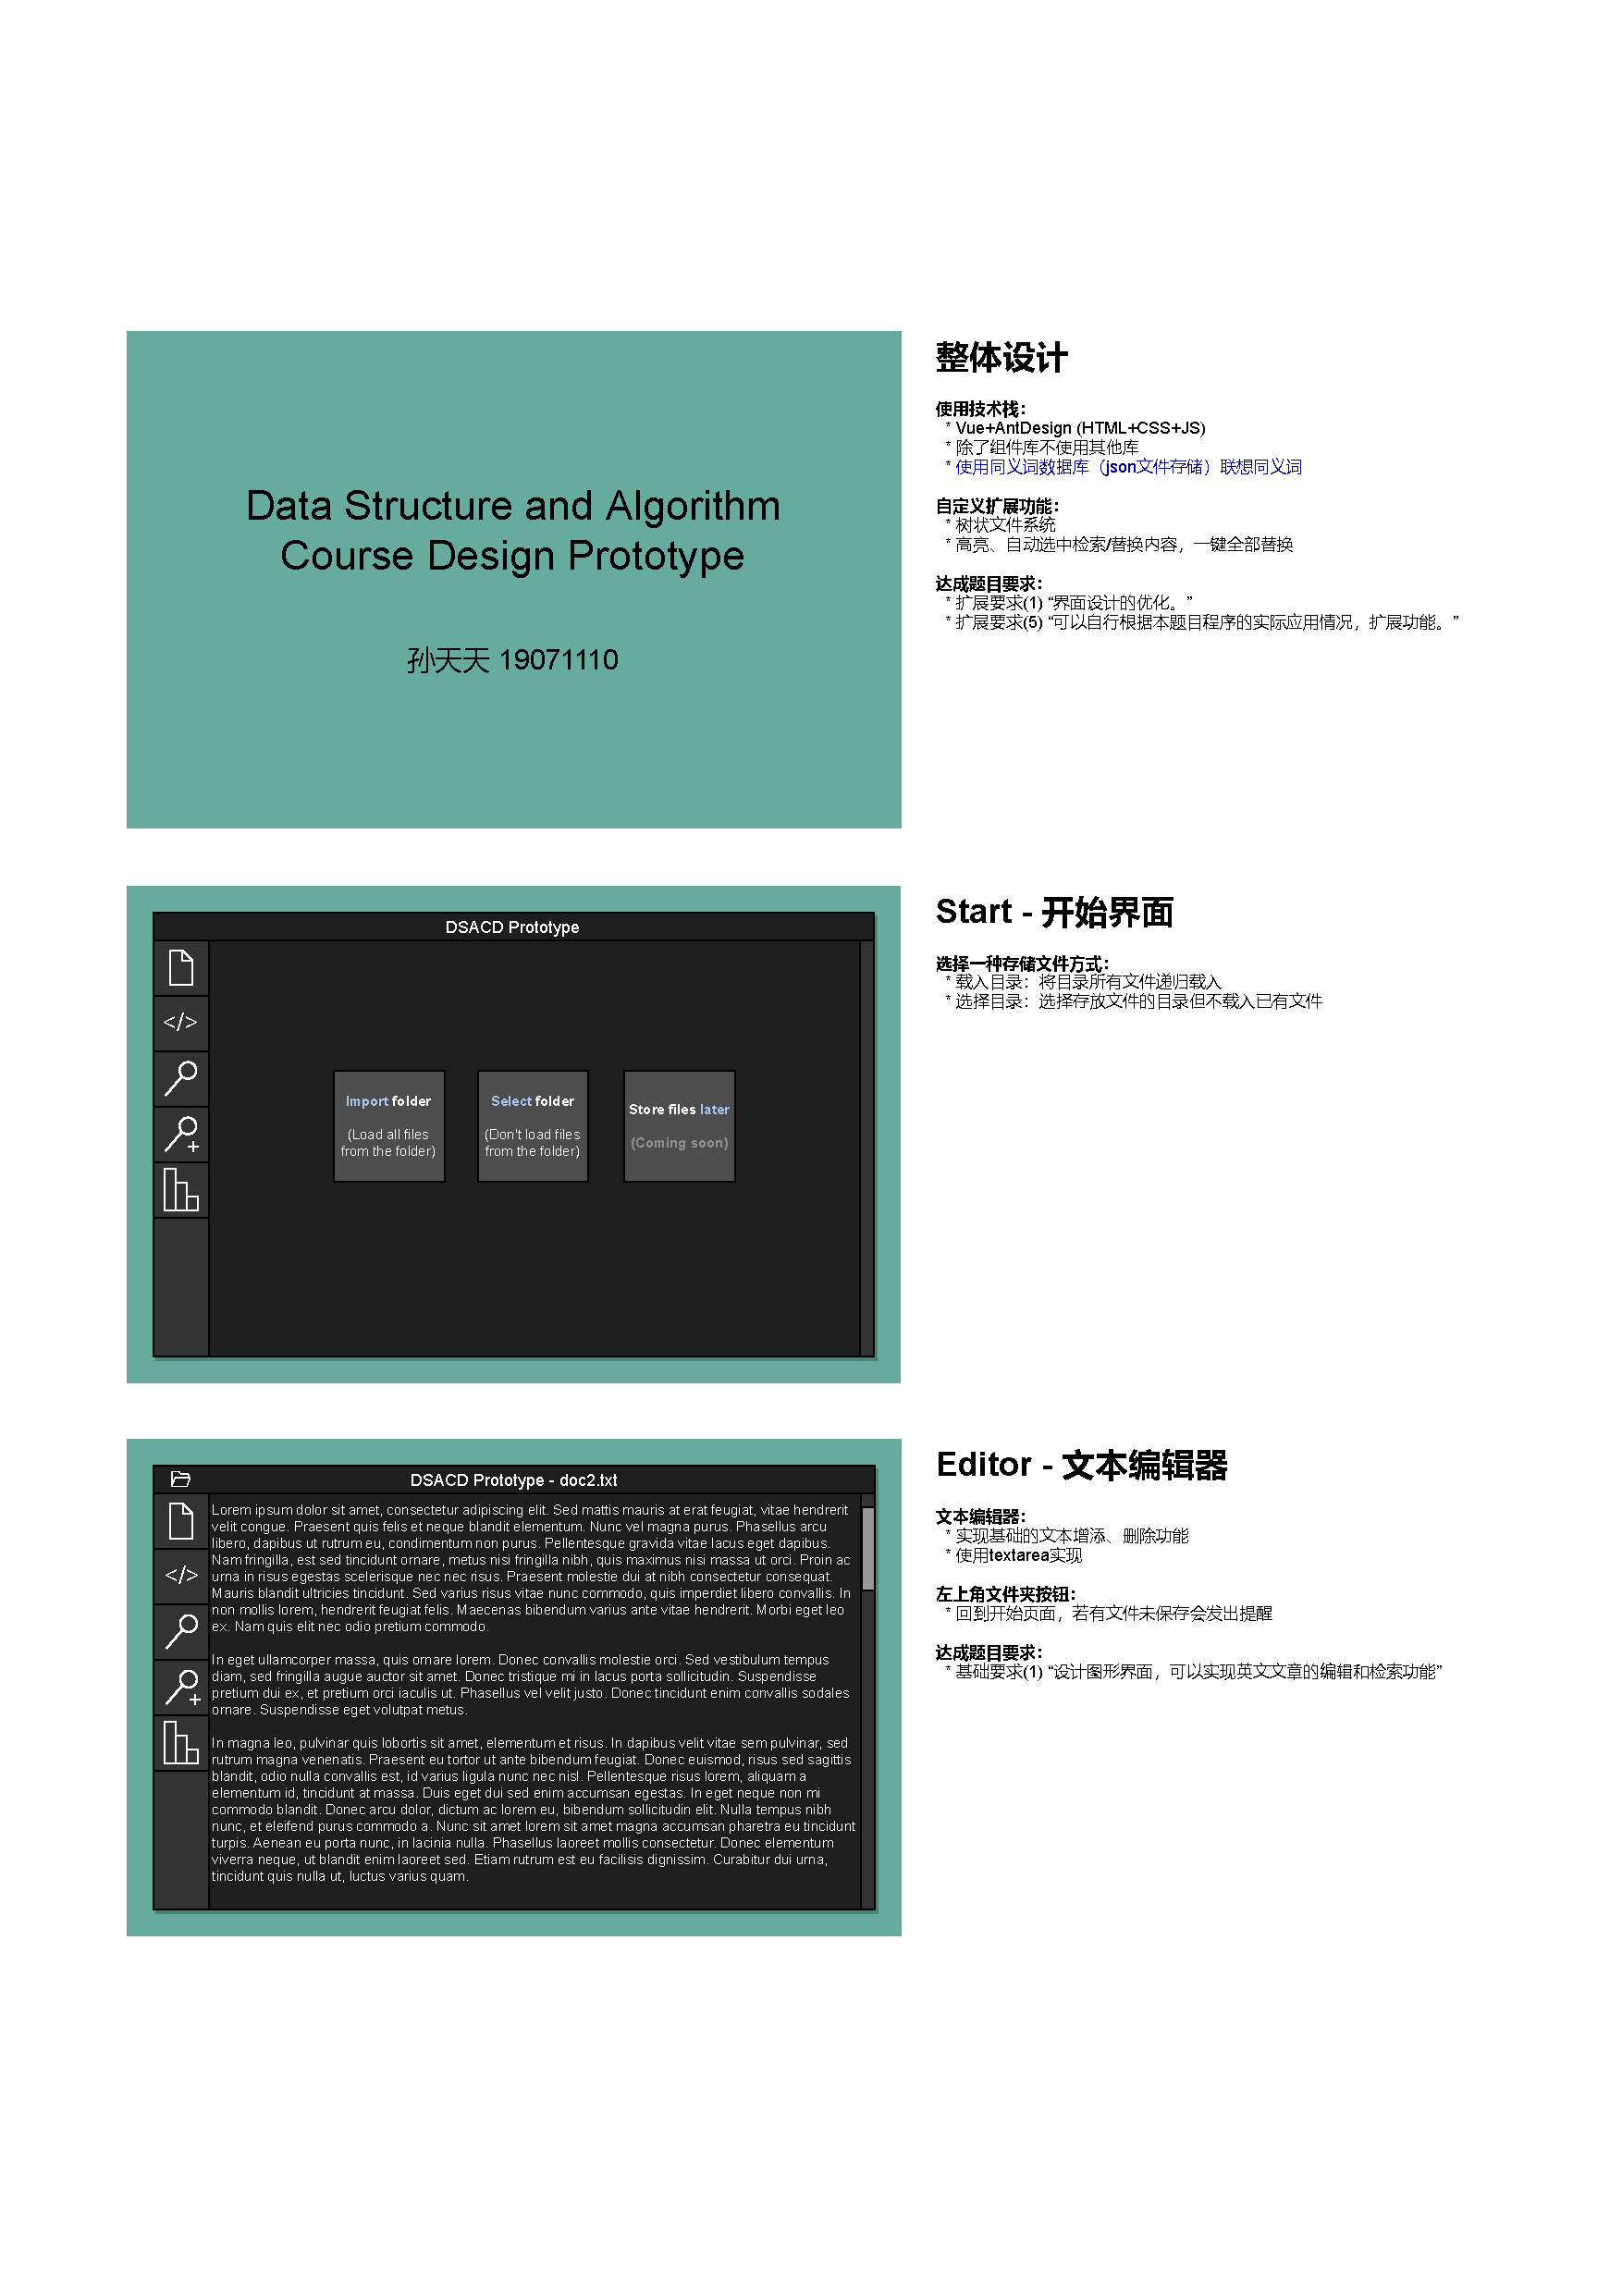
\includepdf[pages=-,pagecommand={},width=1.5\textwidth]{prototype.pdf}

\section{数据结构设计}
此部分要求说明所定义的数据结构和系统的主要模块。这正好对应我\emph{src/lib}目录下作为基础的数据结构模块和\emph{src/components}目录下实现业务逻辑的组件部分。但与数据结构地位相当的一些算法难以恰当地列入这个分类中,为此我增加了所实现的算法部分。下面逐一进行说明。

\subsection{所定义的数据结构}
由于使用JavaScript语言开发,需要首先说明两点:
\begin{outline}
    \1 JavaScript为动态类型语言,以下给出的类型仅为设计中字段应该具有的类型
    \1 JavaScript中的对象操作均为引用,所有对象字段均应理解为对象的引用
\end{outline}

\subsubsection{文件树}
此部分主要在\emph{src/lib/files.js}中,我定义了文件结点类FileNode,每个对应一个文件或目录,以及文件树类FileTree,用来表示一整棵文件树。

\paragraph{FileNode类} 主要包含以下字段:
\begin{table}[H]
    \centering
    \caption{FileNode类的字段}
    \begin{tabular}{ccc}
        \toprule
        字段名 & 类型 & 含义说明 \\
        \midrule
        name & String & 文件或目录名称 \\
        parent & FileNode & 父级目录 \\
        children & FileNode[~] & 子级目录或文件 \\
        handler & FileSystemHandle & 文件API的句柄 \\
        kind & String & 结点类型(文件或目录) \\
        key & String & 唯一标识符 \\
        \midrule
        loaded & Boolean & 文件内容是否已载入 \\
        content & String & 文件内容 \\
        hash & Number & 文件内容哈希值 \\
        lastSavedHash & Number & 上次保存文件时的哈希值 \\
        saved & Boolean & 内容已保存 \\
        workspace & WorkspaceIndex & 全局索引 \\
        \midrule
        unsavedChildren & FileNode Set & 未保存的子目录或文件 \\
        \midrule
        title & String & 显示的文件标题 \\
        slots & Object & 附加显示属性 \\
        \bottomrule
    \end{tabular}
\end{table}

文件结点类FileNode实现了以下功能:
\begin{itemize}
    \item 扫描目录:递归地扫描目录下所有的子目录和文件
    \item 载入、保存:从文件系统中加载、保存到文件系统
    \item 显示保存状态:通过哈希值判断是否已保存,同时递归更新到父结点
    \item 更新索引:内容变化时创新新的倒排索引
\end{itemize}

\paragraph{FileTree类} 包含以下字段:
\begin{table}[H]
    \centering
    \caption{FileTree类的字段}
    \begin{tabular}{ccc}
        \toprule
        字段名 & 类型 & 含义说明 \\
        \midrule
        root & FileNode & 根目录结点 \\
        \bottomrule
    \end{tabular}
\end{table}

文件树类FileTree实现了以下功能:
\begin{itemize}
    \item 打开目录:调用操作系统提供的API打开指定目录并获得读写权限
    \item 扫描目录:从根目录开始递归扫描所有目录
    \item 全部载入、全部保存:递归地载入全部文件(并建立索引)、保存全部文件
\end{itemize}

\subsubsection{哈希表、集合、映射表}
此部分主要在\emph{src/lib/hash.js}中,我定义了哈希表类HashTable,实现了字符串的闭散列,集合类HashSet,用于表示字符串的集合,映射表类HashMap,用于表示字符串到任意对象的映射表(字典)。

\paragraph{HashTable类} 包含以下字段:
\begin{table}[H]
    \centering
    \caption{HashTable类的字段}
    \begin{tabular}{ccc}
        \toprule
        字段名 & 类型 & 含义说明 \\
        \midrule
        capacity & Number & 闭散列最大容量 \\
        array & String[~] & 闭散列数组 \\
        h & function(String) Number & 哈希码函数 \\
        p & function(Number) Nunber & 探查函数 \\
        size & Number & 当前容量 \\
        maxTryTimes & Number & 最大探查次数 \\
        \bottomrule
    \end{tabular}
\end{table}

哈希表类HashTable实现了以下功能:
\begin{itemize}
    \item 创建:支持设定容量和探测函数(内置了线性探测和二次探测)
    \item 查找、获取:查找指定字符串,返回状态或哈希编码
    \item 增加、删除:向哈希表内增加字符串或删除字符串
    \item 转换为广义表:遍历得到所有存储的字符串并转换为广义表
\end{itemize}

\paragraph{HashSet类} 包含以下字段:
\begin{table}[H]
    \centering
    \caption{HashSet类的字段}
    \begin{tabular}{ccc}
        \toprule
        字段名 & 类型 & 含义说明 \\
        \midrule
        hashTable & HashTable & 哈希表 \\
        \bottomrule
    \end{tabular}
\end{table}

集合类HashSet实现了以下功能:
\begin{itemize}
    \item 创建:创建一个集合,调用哈希表实现,还可以从广义表或映射表(只保留键)转换得来
    \item 查找、获取、增加、删除、转换为广义表:调用哈希表实现
    \item 交、并、补:集合的交并补运算
\end{itemize}

\paragraph{HashMap类} 包含以下字段:
\begin{table}[H]
    \centering
    \caption{HashMap类的字段}
    \begin{tabular}{ccc}
        \toprule
        字段名 & 类型 & 含义说明 \\
        \midrule
        hashTable & HashTable & 哈希表 \\
        array & Object[~] & 值数组 \\
        \bottomrule
    \end{tabular}
\end{table}

映射表类HashMap实现了以下功能:
\begin{itemize}
    \item 创建:创建一个映射表,调用哈希表实现
    \item 查找、获取、设置、删除、转换为广义表:调用哈希表实现
    \item 转换为广义表并排序:转换为广义表后,用堆进行排序
\end{itemize}

\subsubsection{堆}
此部分主要在\emph{src/lib/heap.js}中,我定义了堆类Heap,实现了任意类型的堆。

\paragraph{Heap类} 包含以下字段:
\begin{table}[H]
    \centering
    \caption{Heap类的字段}
    \begin{tabular}{ccc}
        \toprule
        字段名 & 类型 & 含义说明 \\
        \midrule
        items & Object[~] & 元素数组 \\
        greater & function(Object, Object) Boolean & 元素比较函数 \\
        size & Number & 当前堆大小 \\
        \bottomrule
    \end{tabular}
\end{table}

堆类Heap实现了以下功能:
\begin{itemize}
    \item 创建:由任意类型数组创建堆,同时提供比较函数
    \item ShiftDown、ShiftUp:实现两种维护有序性的转移操作
    \item 压入、弹出:压入或弹出元素的同时维护堆的有序性
    \item 堆排序:数组建堆后逐一弹出实现排序
\end{itemize}

\subsubsection{哈夫曼树}
此部分主要在\emph{src/lib/huffman.js}中,我定义了哈夫曼结点类HuffmanNode和哈夫曼树类HuffmanTree,实现了哈夫曼编码和译码。

\paragraph{HuffmanNode类} 包含以下字段:
\begin{table}[H]
    \centering
    \caption{HuffmanNode类的字段}
    \begin{tabular}{ccc}
        \toprule
        字段名 & 类型 & 含义说明 \\
        \midrule
        char & Number & \makecell[ct]{
        表示字符的ASCII码 \\
        {\small(中间结点为-1)} \\
        } \\
        weight & Number & 权重 \\
        children & HuffmanNode[~] & 子节点 \\
        parent & HuffmanNode & 父节点 \\
        code & String & 编码结果 \\
        \bottomrule
    \end{tabular}
\end{table}

哈夫曼结点类HuffmanNode实现了以下功能:
\begin{itemize}
    \item 创建:创建为对应字符的叶子结点或中间结点
    \item 合并:构造两个哈夫曼结点的父结点
\end{itemize}

\paragraph{HuffmanTree类} 包含以下字段:
\begin{table}[H]
    \centering
    \caption{HuffmanTree类的字段}
    \begin{tabular}{ccc}
        \toprule
        字段名 & 类型 & 含义说明 \\
        \midrule
        root & HuffmanNode & 根目录结点 \\
        \bottomrule
    \end{tabular}
\end{table}

哈夫曼树类HuffmanTree实现了以下功能:
\begin{itemize}
    \item 由字符和频率创建:根据字符和频率先生成叶子结点再逐步合并生成一棵树
    \item 由对应表导入:根据字符和前缀码通过前序遍历生成一棵树
    \item 生成对应表:遍历树来实现字符和前缀码的对应表
    \item 生成图数据:中序遍历树生成可视化使用的结点关系和坐标
\end{itemize}

由哈夫曼树类,可实现哈夫曼编码译码功能:
\begin{itemize}
    \item 编码:由字符和频率创建树,生成对应表和编码后的比特流
    \item 译码:由对应表创建树,生成译码后的文段
\end{itemize}

\paragraph{base64类} 为静态类,不包含字段。

\subsubsection{base64编解码器}
此部分主要在\emph{src/lib/base64.js}中,我定义了静态的Base64编解码类base64。

Base64编解码类base64实现了以下功能:
\begin{itemize}
    \item 编码:将任意比特流编码为base64形式
    \item 解码:将base64形式字符串解码为比特流
\end{itemize}

\subsubsection{替换器}
此部分主要在\emph{src/lib/KMP.js}中,我定义了替换器类Replacer,实现了自动修正位置的单次替换、迭代器式替换、全部替换。

\paragraph{KMP算法}
替换器依赖于KMP算法,因此需要先介绍实现的KMP算法:
\begin{itemize}
    \item prefixFunction函数:生成前缀数组
    \item findAll函数、split函数:基于前缀数组实现字符串匹配、拆分
\end{itemize}

\paragraph{Replacer类} 包含以下字段:
\begin{table}[H]
    \centering
    \caption{Replacer类的字段}
    \begin{tabular}{ccc}
        \toprule
        字段名 & 类型 & 含义说明 \\
        \midrule
        str & String & 处理的字符串 \\
        source & String & 替换前的关键词 \\
        target & String & 替换后的关键词 \\
        lastReplaced & Number & 上次替换位置 \\
        \bottomrule
    \end{tabular} \\~\\
    {\small 
注:替换器Replacer从source关键词替换为target关键词。}
\end{table}

替换器类Replacer实现了以下功能:
\begin{itemize}
    \item 查找:查找所有匹配位置
    \item 单次替换:替换当前位置,并记录文本长度变化,保证下一次替换位置正确
    \item 全部替换:不断调用单次替换直到全部替换完成
\end{itemize}

\subsubsection{倒排索引}
此部分主要在\emph{src/lib/invertedIndex.js}中,我定义了文件索引类FileIndex,实现了对单文件内各个单词位置的索引和多文件索引类WorkspaceIndex,实现了对单文件索引的索引。整体结构为一个二级索引。

\paragraph{FileIndex类} 包含以下字段:
\begin{table}[H]
    \centering
    \caption{FileIndex类的字段}
    \begin{tabular}{ccc}
        \toprule
        字段名 & 类型 & 含义说明 \\
        \midrule
        map & HashMap & 词到词位置与词频的映射表 \\
        hash & Number & 索引内容的哈希码 \\
        workspace & WorkspaceIndex & 全局索引 \\
        fileNode & FileNode & 文件结点 \\
        \bottomrule
    \end{tabular}
\end{table}

文件索引类FileIndex实现了以下功能:
\begin{itemize}
    \item 创建:根据文件内容(字符串)创建倒排索引,每次文件内容变化时重新创建。
    \item 获取词频TF:实现词频统计,可以方便地获取某文件内指定词的词频
    \item 获取位置:获取某文件内指定词出现的各个位置
\end{itemize}

\paragraph{WorkspaceIndex类} 主要包含以下字段:
\begin{table}[H]
    \centering
    \caption{WorkspaceIndex类的字段}
    \begin{tabular}{ccc}
        \toprule
        字段名 & 类型 & 含义说明 \\
        \midrule
        map & HashMap & 词到各文件词频和总词频的映射表 \\
        filesIndexes & HashMap & 内容哈希到文件索引的映射表 \\
        \bottomrule
    \end{tabular}
\end{table}

多文件索引类WorkspaceIndex实现了以下功能:
\begin{itemize}
    \item 增、删文件索引:增添包含的文件索引,使用文件哈希作一致性判断
    \item 统计词频:索引文件索引的同时,统计多文件整体的词频
    \item 获取逆文本频率指数IDF:根据多文件TF计算指定词的IDF值
\end{itemize}

\subsection{所实现的算法}

\subsubsection{表达式转换与求值}
此部分主要在\emph{src/lib/expression.js}中,我实现了中缀转后缀表达式InFixExpressionToPostfix和后缀表达式求值ExecutePostfixExpression。

\paragraph{中缀转后缀表达式InFixExpressionToPostfix算法} 使用一个运算符堆栈实现,可以实现支持单种括号匹配、运算符优先级的中缀表达式转后缀表达式。

\paragraph{后缀表达式求值ExecutePostfixExpression算法} 使用一个运算数堆栈实现,可以实现自定义运算符、运算函数的后缀表达式求值。

\subsubsection{高级检索}
此部分主要在\emph{src/lib/advancedSearch.js}中,我主要实现了匹配文档集合运算CalculateSet、相关性权重计算calculateWeight、同义词扩展AddSynonyms。

\paragraph{匹配文档集合运算CalculateSet算法} 将检索表达式中的AND,OR,NOT视为求交集、求并集和全集求补集运算,筛选出匹配的文档。

\paragraph{相关性权重计算calculateWeight算法} 将检索表达式中的AND,OR,NOT视为求最小值、求最大值和求差值运算,计算出各个文档的相关性权重。

\paragraph{同义词扩展AddSynonyms算法} 启用同义词拓展时,将每个检索关键词转换为其本身和同义词相或的表达式,再进行计算。

\subsection{系统整体结构以及各模块的功能描述}
此部分将系统按功能分为大体模块,并描述每个模块。这种划分与我使用Vue框架对系统进行组件划分的思路基本一致,因此以下按组件划分进行说明。

\subsubsection{整体组件App}
整个系统均包含在这个组件中,它复制系统组件间的信息通讯、页面整体布局、全局初始化等功能。

下图中展示了整体的布局,可见界面首先在上、下切出了两块页眉Header和页脚Footer部分;之后再从左到右划分为侧栏切换菜单Menu、侧栏Side Bar和编辑器栏Editor Bar。

其中,侧栏和编辑器栏可以切换不同的功能。侧栏使用左侧的侧栏切换菜单进行切换,侧栏和编辑器栏的占比可以随意调整,也可以彻底收起侧栏;而编辑器栏会自动根据当前选择的文件或目录情况进行切换。

下面前四个以“界面”结尾的组件均用于编辑器栏,而后面五个以“侧栏"结尾的组件均用于侧栏。

\begin{figure}[h]
    \centering
    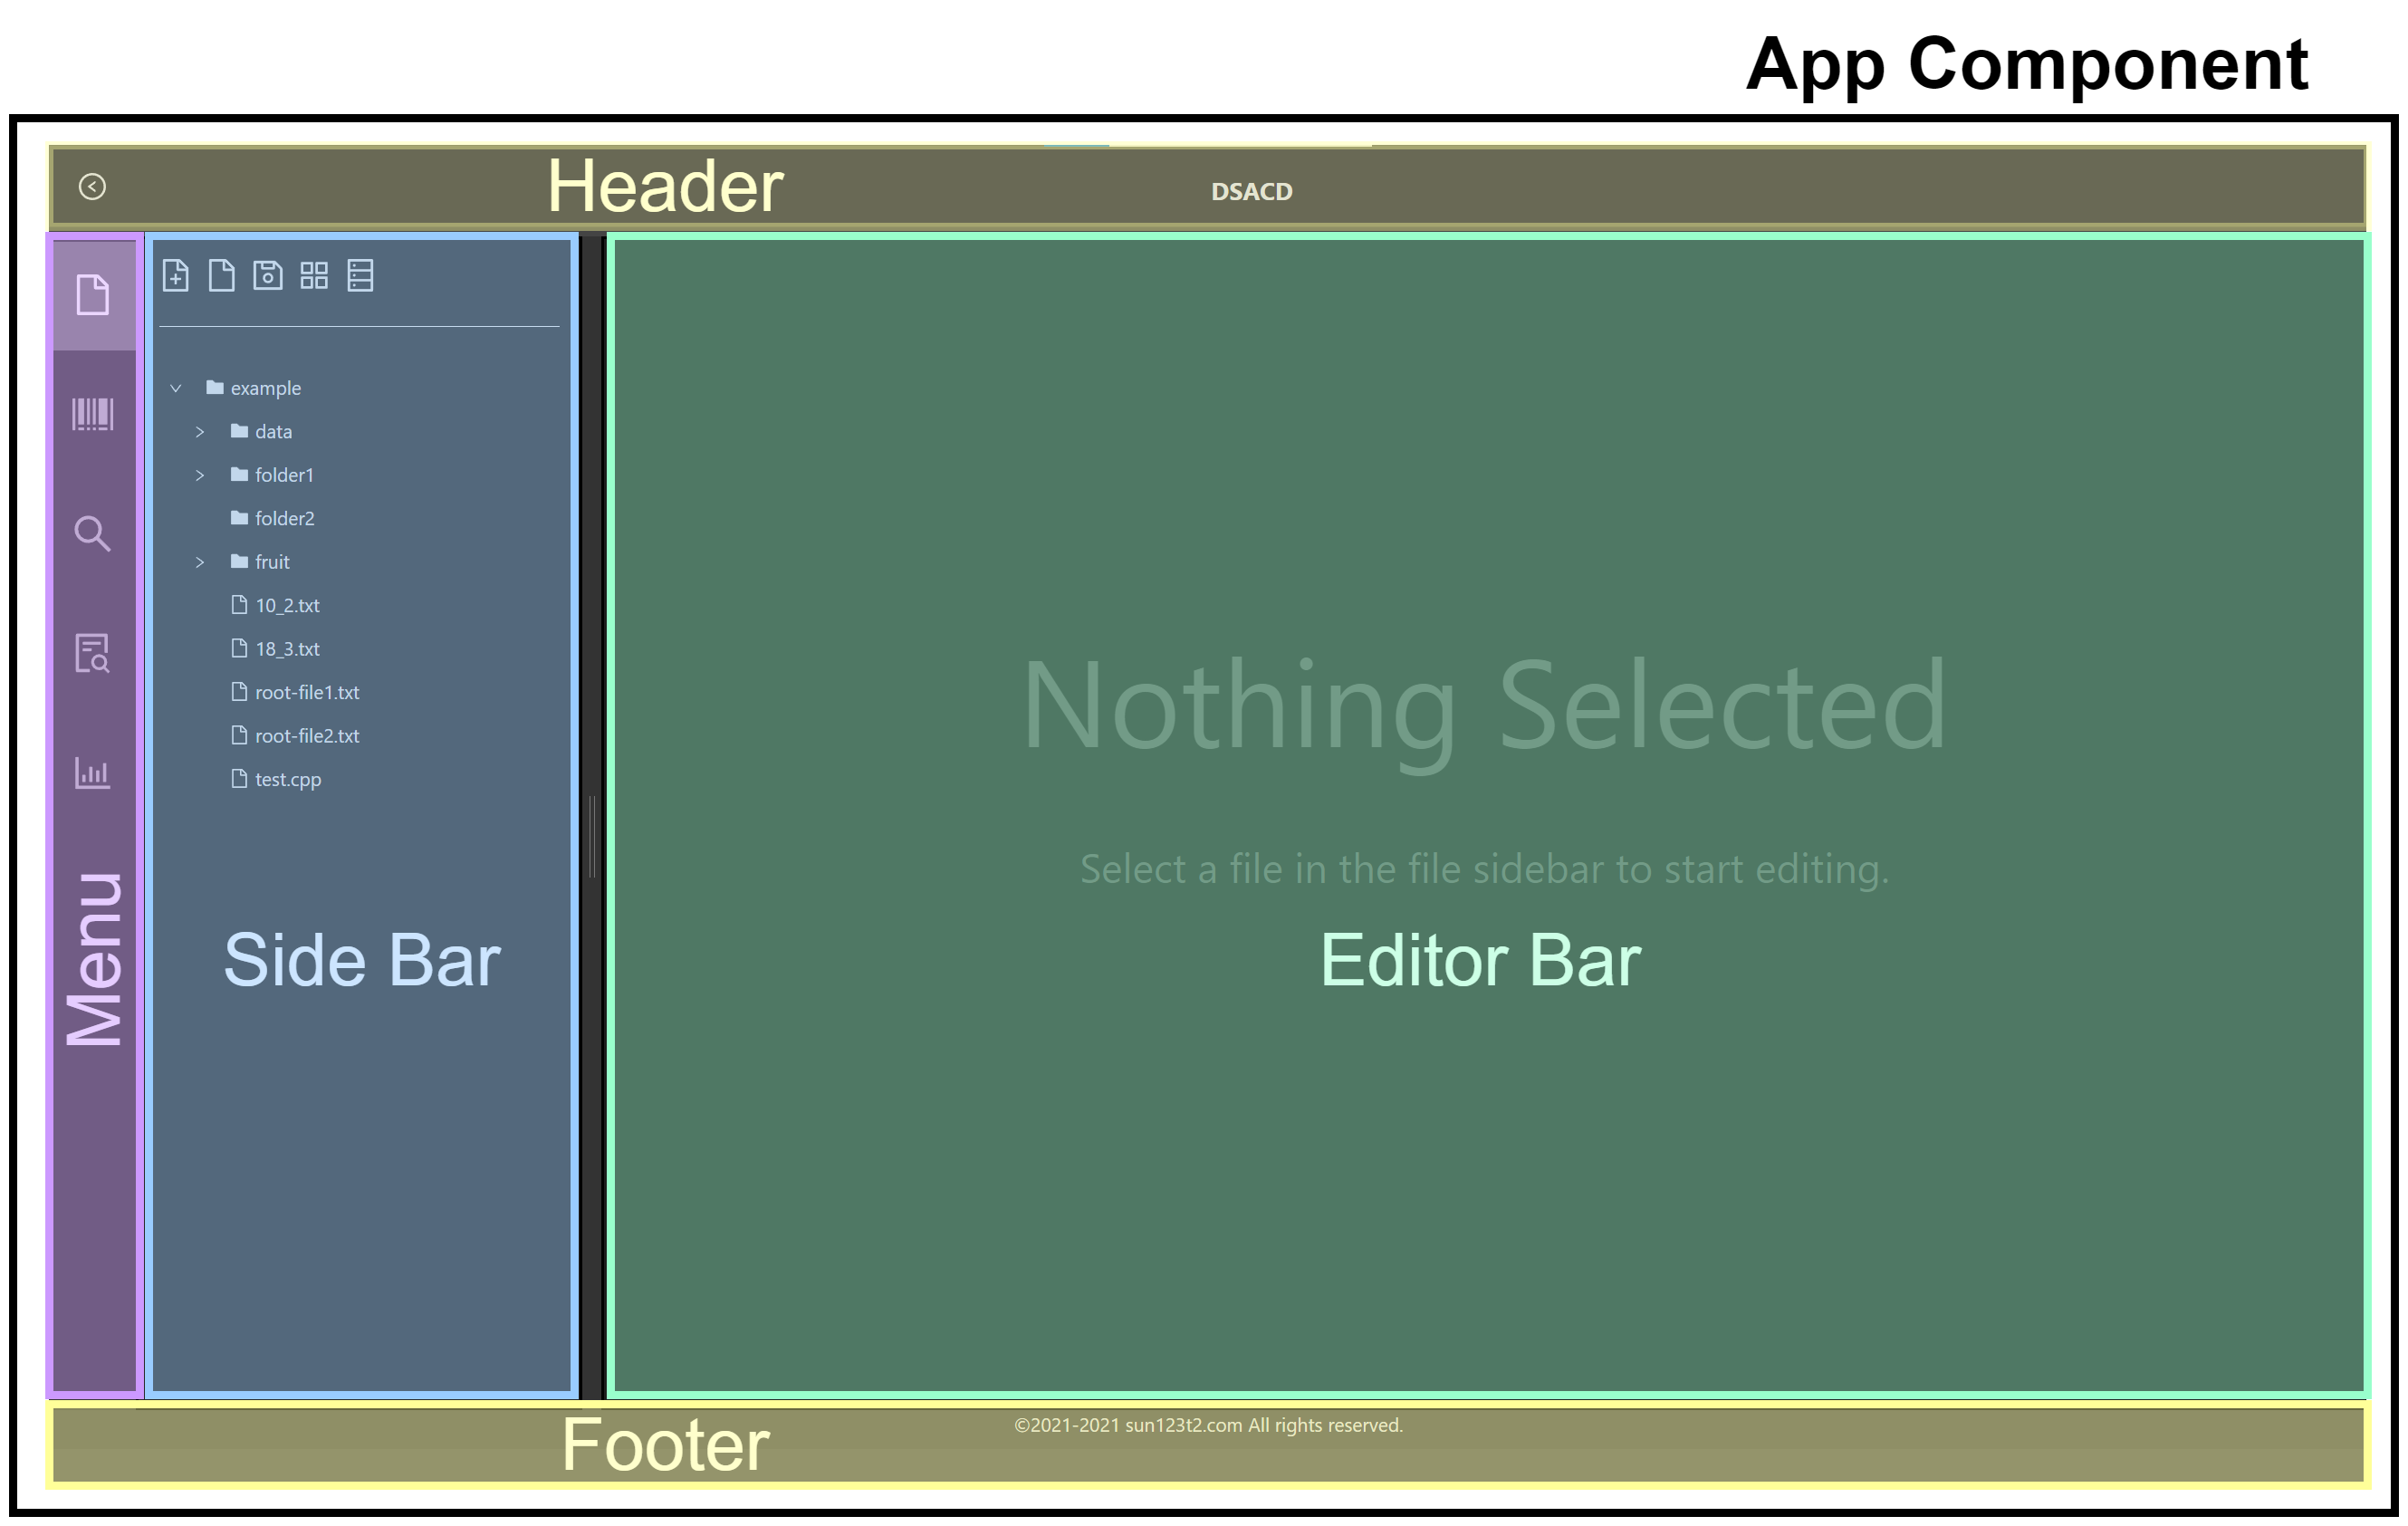
\includegraphics[width=\textwidth]{images/dsacd-screenshot-layout.drawio.png}
    \caption{整体布局}
\end{figure}

\subsubsection{开始界面StartPanel}
进入系统后,用户侧栏关闭,并进入开始界面。必须选择打开某文件夹及其内部内容,或选择某文件夹作为存储位置(不扫描其内部内容)。在选择文件夹前无法进行其他操作,包括打开侧栏和任何文件编辑功能。

\paragraph{打开文件夹Import folder}
该功能会创建文件树、创建多文件索引,并递归地扫描目录以创建文件树中各结点(并不会读取文件内容)。
完成以上工作后,会自动切换到文件侧栏和空白界面,引导用户开始编辑文件。

\paragraph{选择存储目录Select folder}
该功能与打开文件夹类似,只是不会递归扫描目录,仅创建选择的文件夹作为文件树的根节点。

\begin{figure}[h]
    \centering
    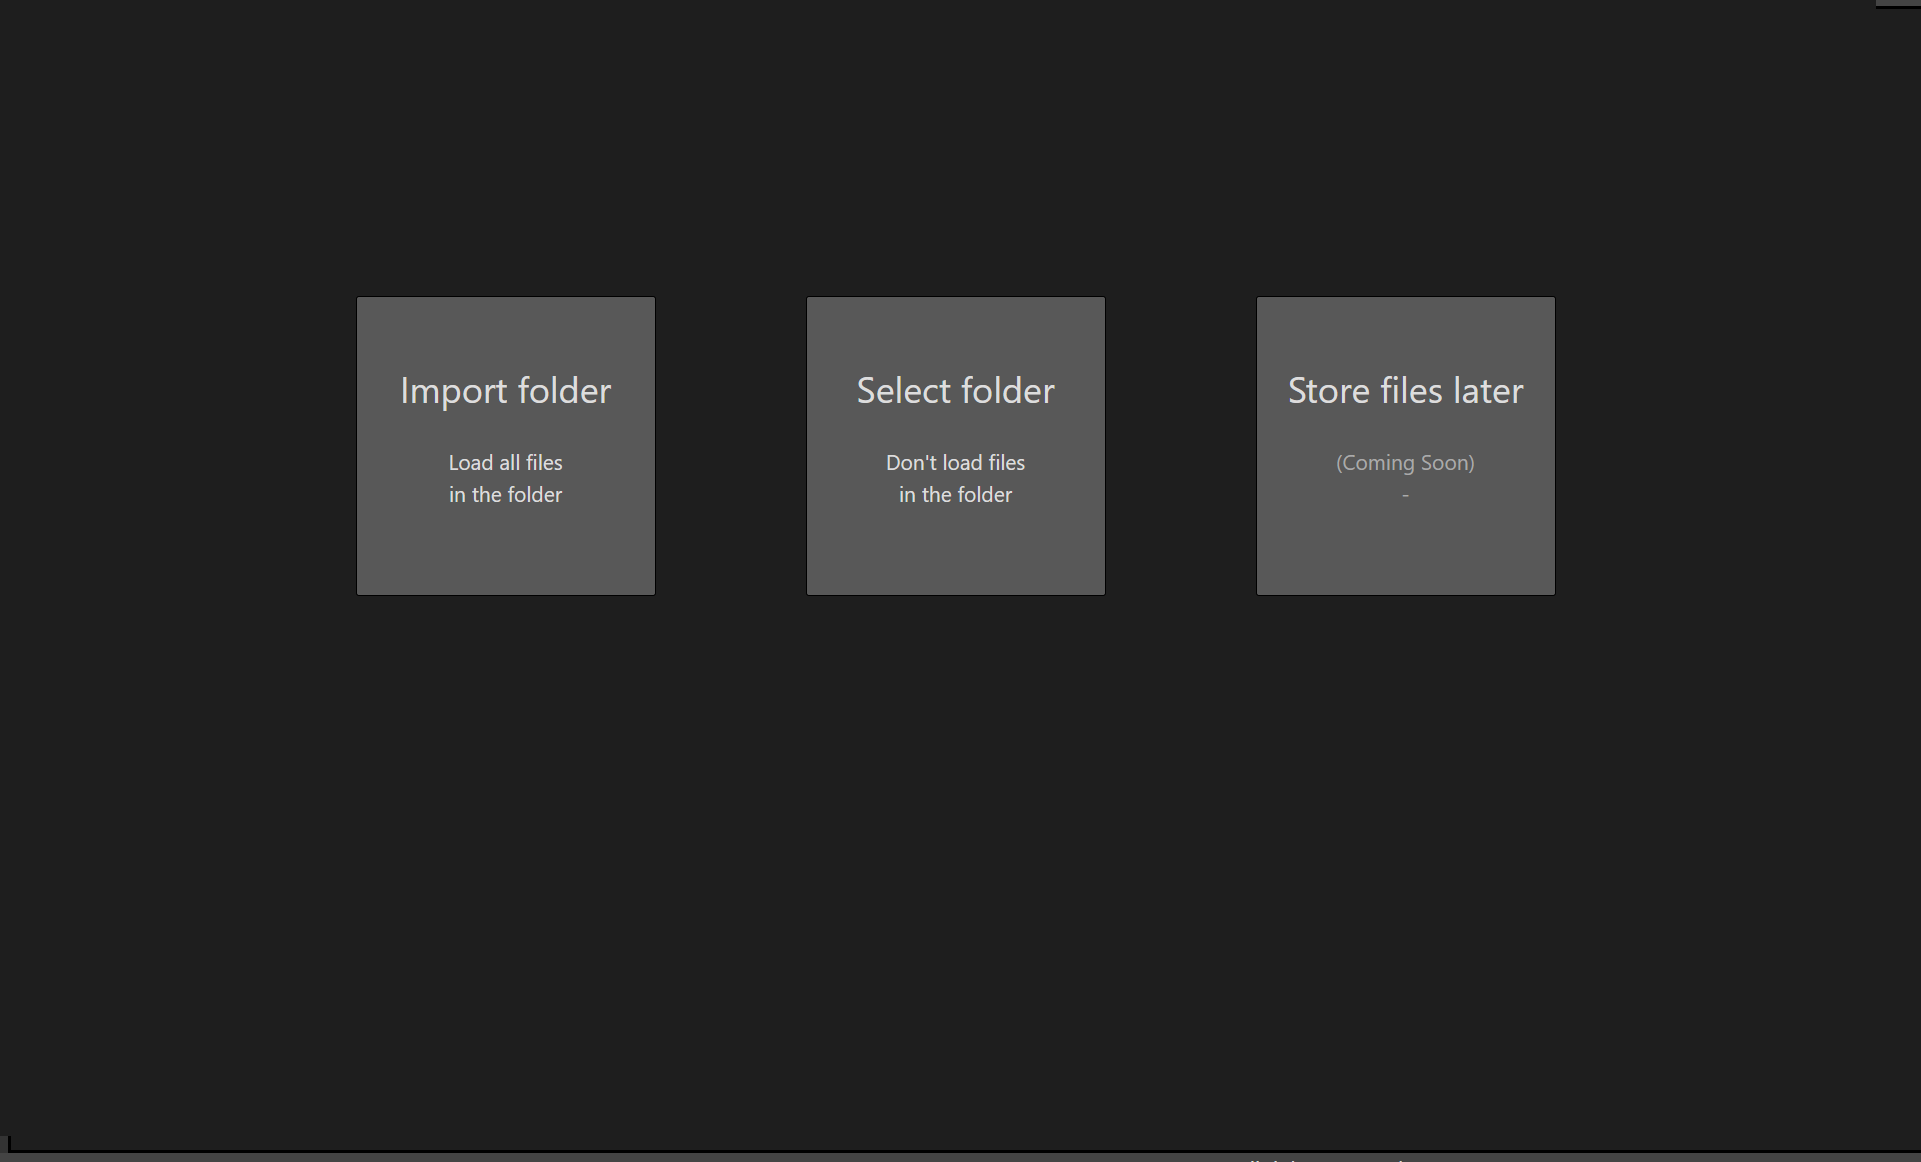
\includegraphics[width=0.8\textwidth]{images/StartPanel.png}
    \caption{开始界面}
\end{figure}

\subsubsection{空白界面DummyEditorBar}
当用户未选择任何文件时,右侧会显示空白界面,提示用户从左侧的文件侧栏选择文件。

\begin{figure}[h]
    \centering
    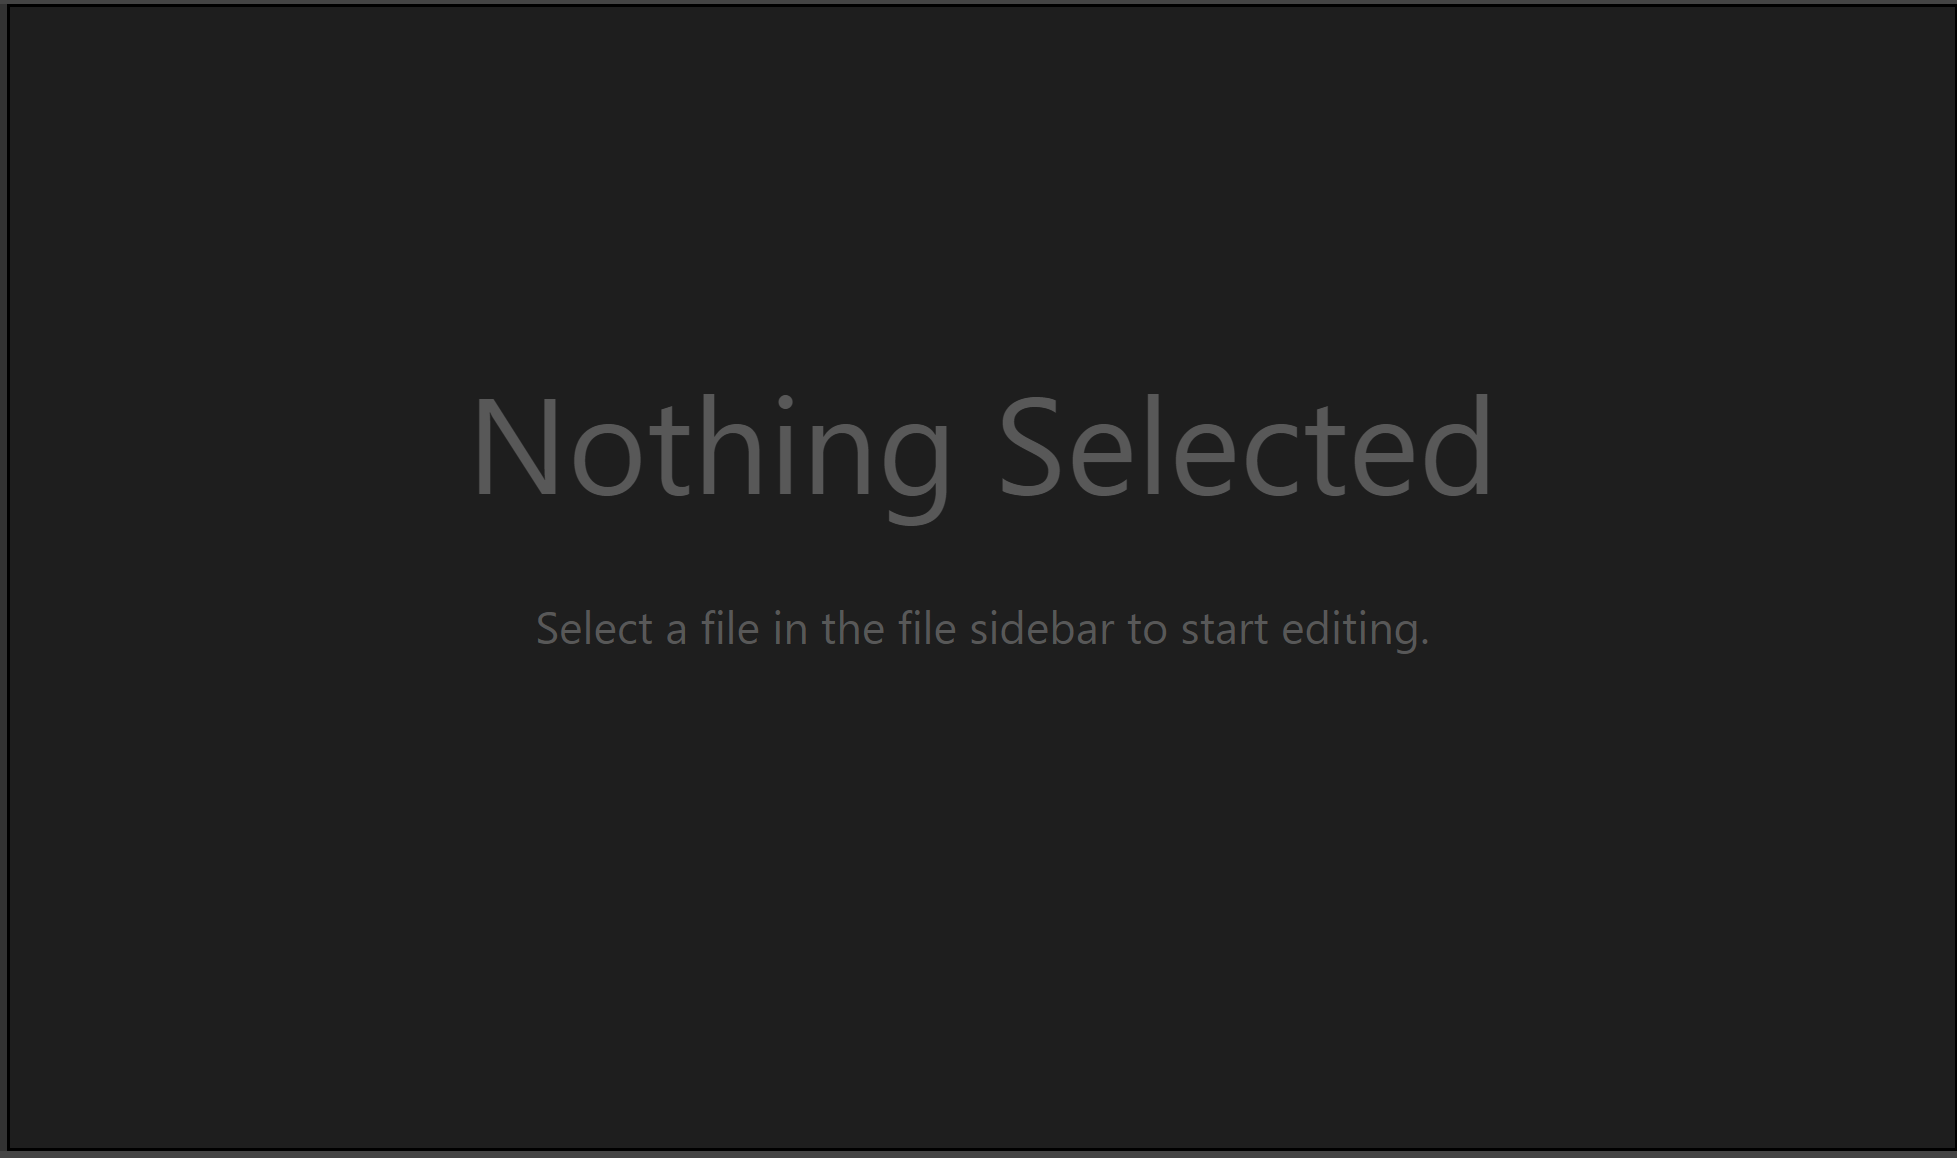
\includegraphics[width=0.8\textwidth]{images/DummyEditorBar.png}
    \caption{空白界面}
\end{figure}

\subsubsection{编辑器界面Editor}
当用户选择一个文件后,会自动切换到此界面。用户可以在其中随意修改文件中的文本内容。此外,编辑器界面还提供以下功能和其他模块交互。
\begin{itemize}
    \item 内容更新通知:主要用于和文件模块交互,当文件内容被改变,且用户失去编辑器焦点或切换文件时,会向文件模块传递信息以更新文件未保存状态
    \item 文件切换:切换文件时,会自动缓存前一个文件,并打开另一个文件
    \item 内容选取:可以根据开始和终止位置自动选取指定位置的文字
    \item 内容提取和覆盖:可以对出用户当前选中的文字进行提取或覆盖
\end{itemize}

\begin{figure}[h]
    \centering
    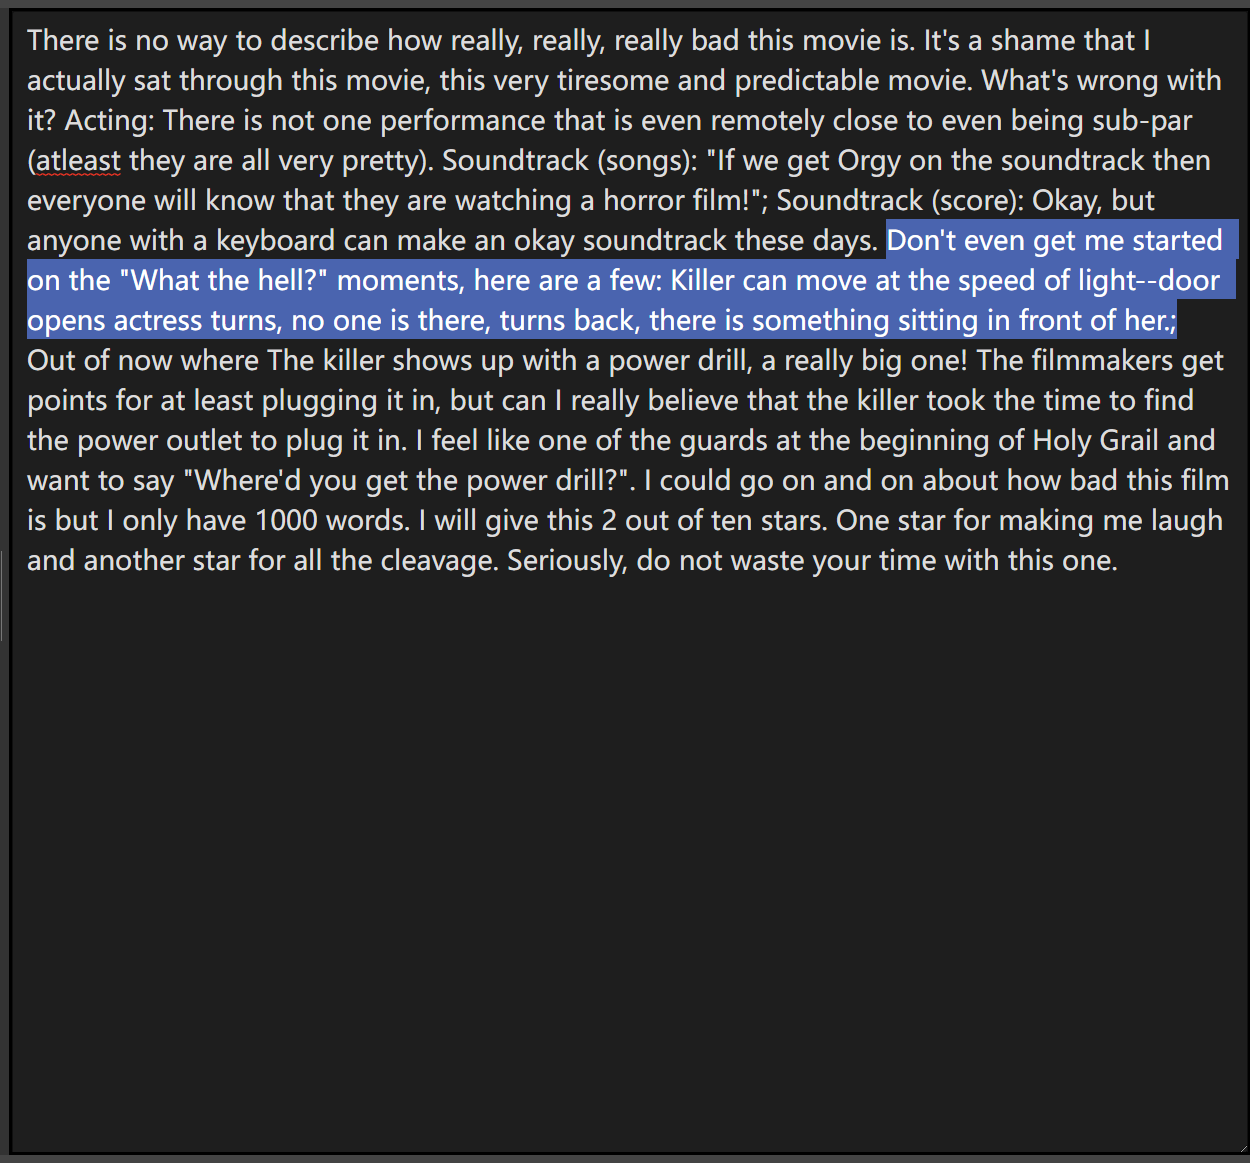
\includegraphics[width=\textwidth]{images/Editor.png}
    \caption{编辑器界面}
\end{figure}

\clearpage

\subsubsection{目录预览界面DivViewer}
当用户选择一个文件后,会自动切换到此界面。此界面会预览此目录直接包含的目录和文件,若较多则仅显示前5个。

\begin{figure}[h]
    \centering
    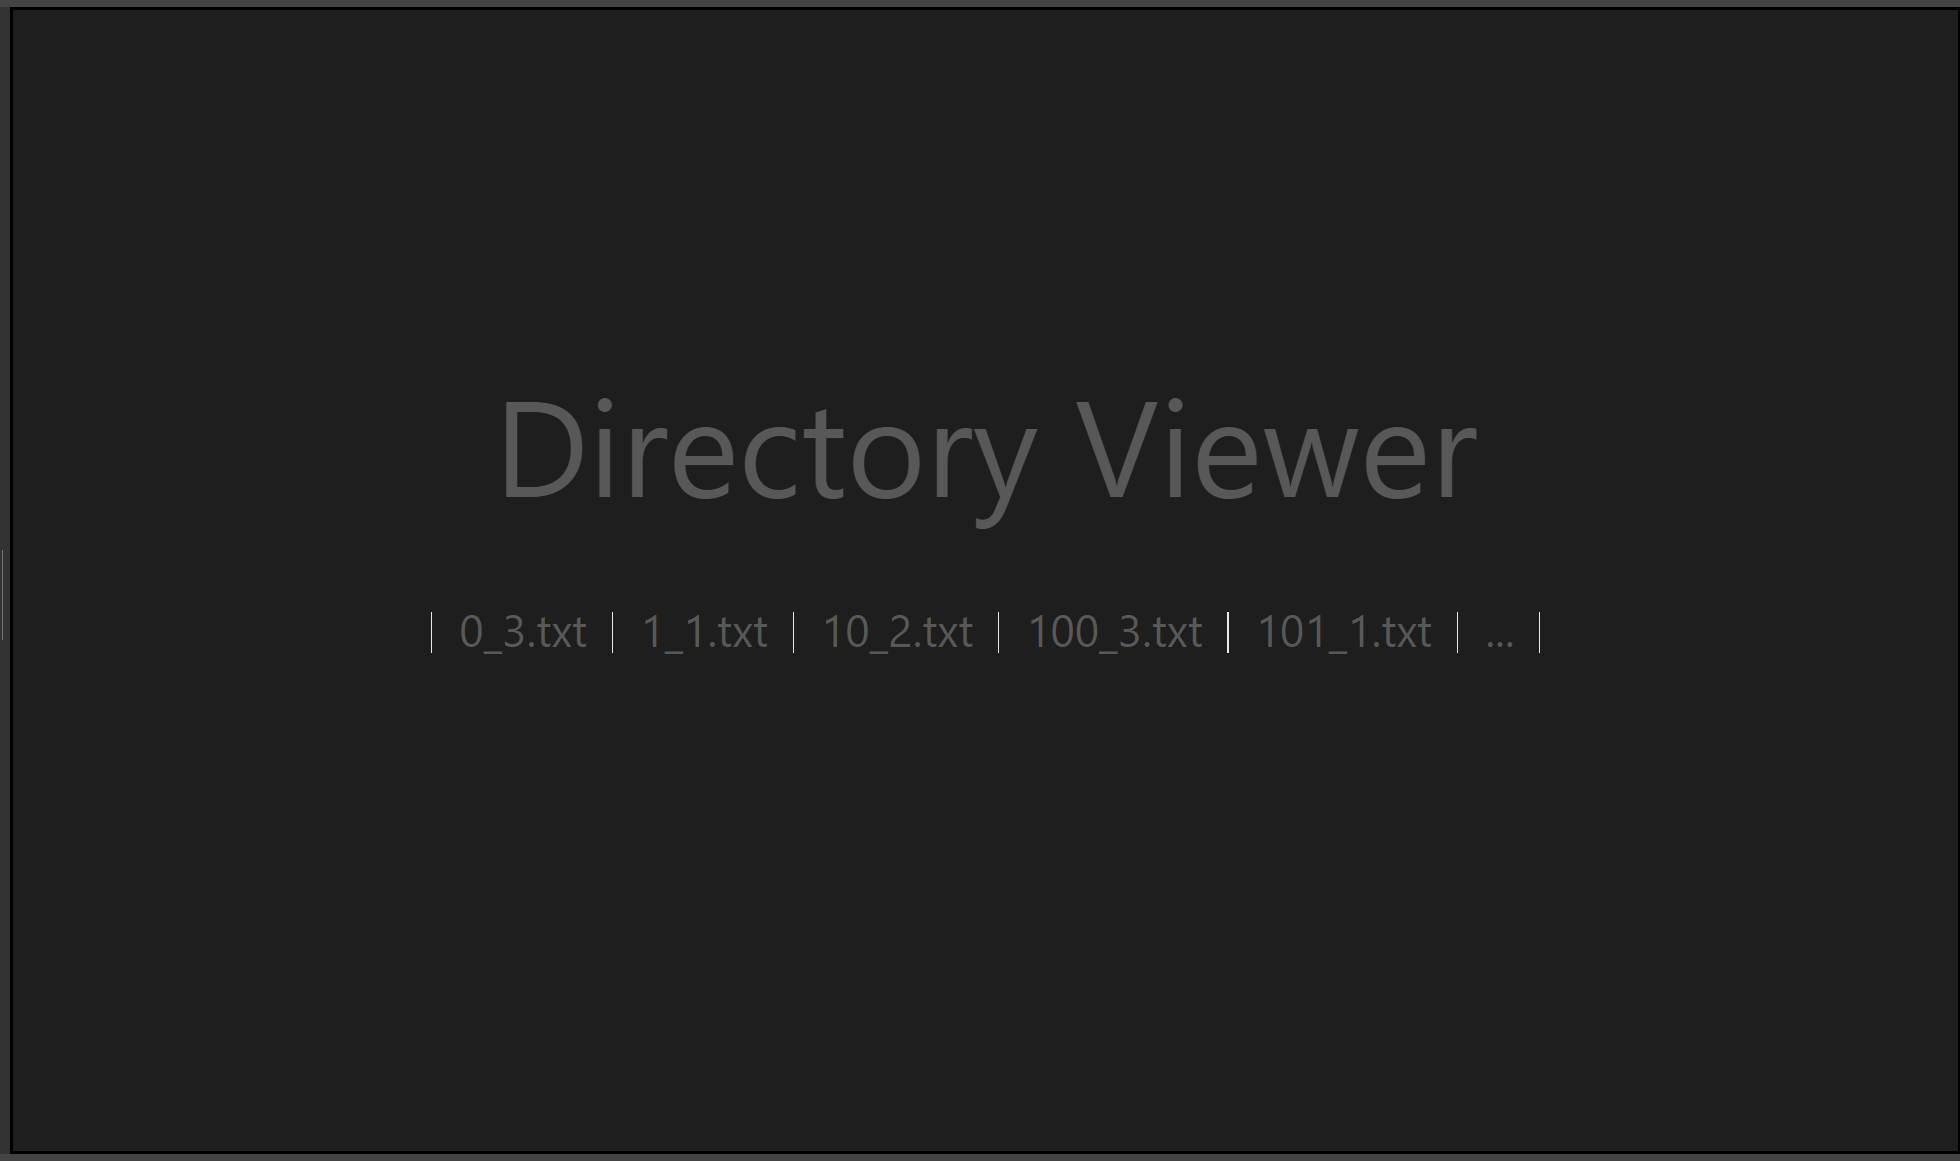
\includegraphics[width=0.6\textwidth]{images/DivViewer.png}
    \caption{目录预览界面}
\end{figure}


\subsubsection{文件侧栏FileButtons和FileTree}
文件侧栏可分为FileButtons和FileTree两个部分,中间有一条分界线用于划分。

\paragraph{文件操作按钮FileButtons} 用于实现文件的创建、打开、保存、全部保存和未保存信息更新。

操作的目录称为“当前目录”,在选中文件时是选中文件同目录,选中目录时是选中的目录,未选中时是根目录。
具体功能如下:
\begin{itemize}
    \item 新建文件:网页内弹出窗口输入名称,在当前目录下新建文件。
    \item 打开文件:打开磁盘任意位置文件,并将其放入当前目录。
    \item 保存文件:保存当前打开的文件。
    \item 全部保存:保存所有未保存的文件。
    \item 更新未保存状态:更新所有文件的未保存状态(所有文件检查哈希)。
\end{itemize}

\begin{figure}[h]
    \centering
    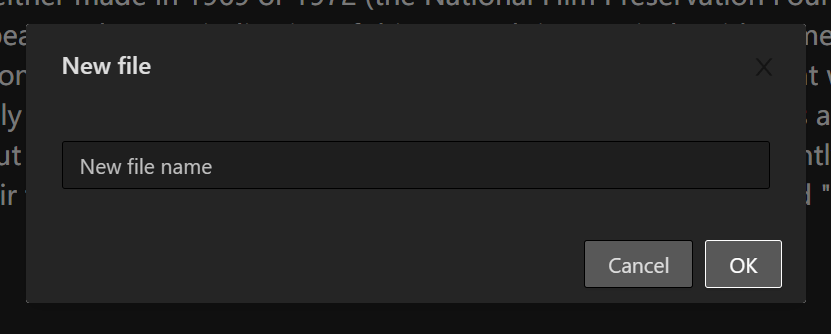
\includegraphics[width=0.6\textwidth]{images/new-file.png}
    \caption{新建文件的网页内弹窗}
\end{figure}

\paragraph{文件树 FileTree} 用于树状展示文件的目录结构,选择当前编辑的文件,可收起或展开任意一个目录结点。

如下图中的左图展示了该模块树状展示文件目录结构,选择指定文件或目录的功能。
当进行文件切换时,会自动切换编辑器栏,对应无选择、选择文件、选择目录,显示空白界面、编辑器界面、目录预览界面。
切换到未载入的文件时,会先进行载入和索引。

如下图中的右图展示了标记未保存文件的功能。未保存的文件会被标为蓝色,同时其祖先目录也都会被标为蓝色。这样的设计主要用于解决文件被因此的情况(如图中的file文件夹,内部有文件未保存可以通过文件夹的蓝色发现)。

\begin{figure}[h]
    \centering
    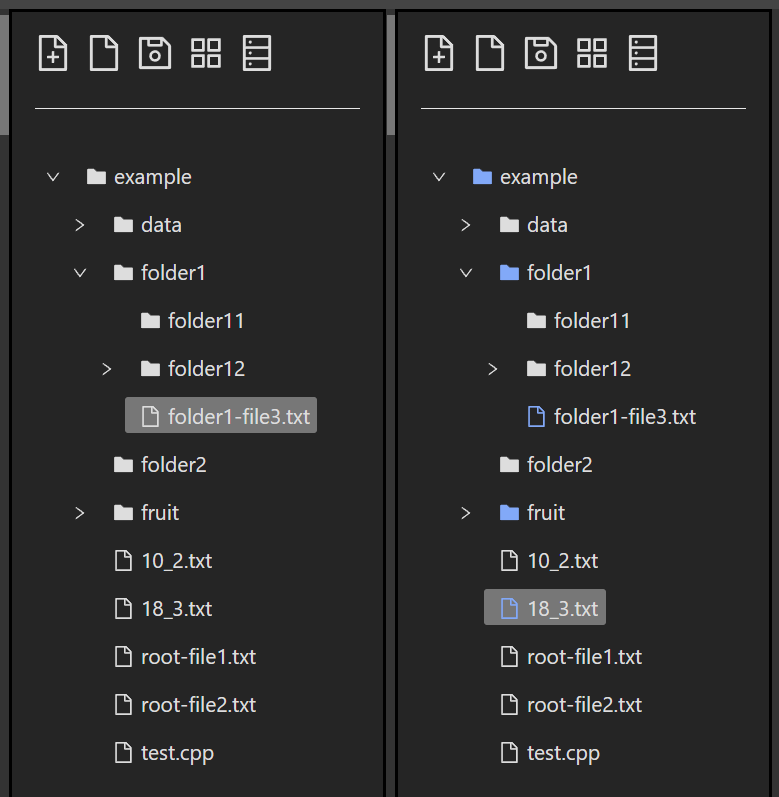
\includegraphics[width=\textwidth]{images/File.png}
    \caption{文件侧栏}
\end{figure}

\clearpage

\subsubsection{编码译码侧栏EncodingPanel}
编码译码侧栏如下图所示,分为原文Conternt、哈夫曼编码比特流Code、哈夫曼编码后base64结果Code+base64、哈夫曼编码对应表CodingMap几部分。这几部分之间相互关联,下面具体阐述。

\paragraph{Content和编辑器中选中的文字}
原文文本框下方有两个按钮,其中Load表示将编辑器中选中的部分放到原文这里,而Store表示将原文内容替换掉编辑器中。

\paragraph{Code和它的base64编码Code+base64}
这两个文本框时刻保证一致性。当Code发生变化时,会自动编码base64更新Code+base64,反之当Code+base64发生变化时也会自动解码base64更新Code。

base64原本是对任意ASCII字符串进行编码,可以生成只由64种字符组成的字符串。而我这里对它进行了改造,可以对任意比特流编码为仅由64种字符组成的字符串。具体而言,对于任意比特流,首先要将其对齐到8的整数倍长度。为此我设定每个比特流前面增加一串数个0和一个1的填充部分,根据比特流长度不同填入1至8个比特。这样即可以顺利地进行base64编解码了。

\paragraph{Content、Code和CodingMap}
这三者之间的关系就是哈夫曼编解码的关系。Content处输入任意原文,系统会自动统计符号频率并生成它的哈夫曼编码Code和字符编码对应表CodingMap。反过来,当输入对应表CodingMap和哈夫曼编码Code时,可以解码处原文Content。编码和解码的过程分别由下方的按钮触发。

\paragraph{哈夫曼树可视化}
只有对应表CodingMap非空,点击显示哈夫曼树的按钮即可出现一个页内弹窗显示哈夫曼树。这个哈夫曼树的结点位置通过中序遍历生成,每两个中序遍历相邻的结点距离一定。展示的哈夫曼树显示各结点前缀码、权重和叶子结点代表的字符,可以用鼠标缩放、移动。

\begin{figure}[h]
    \centering
    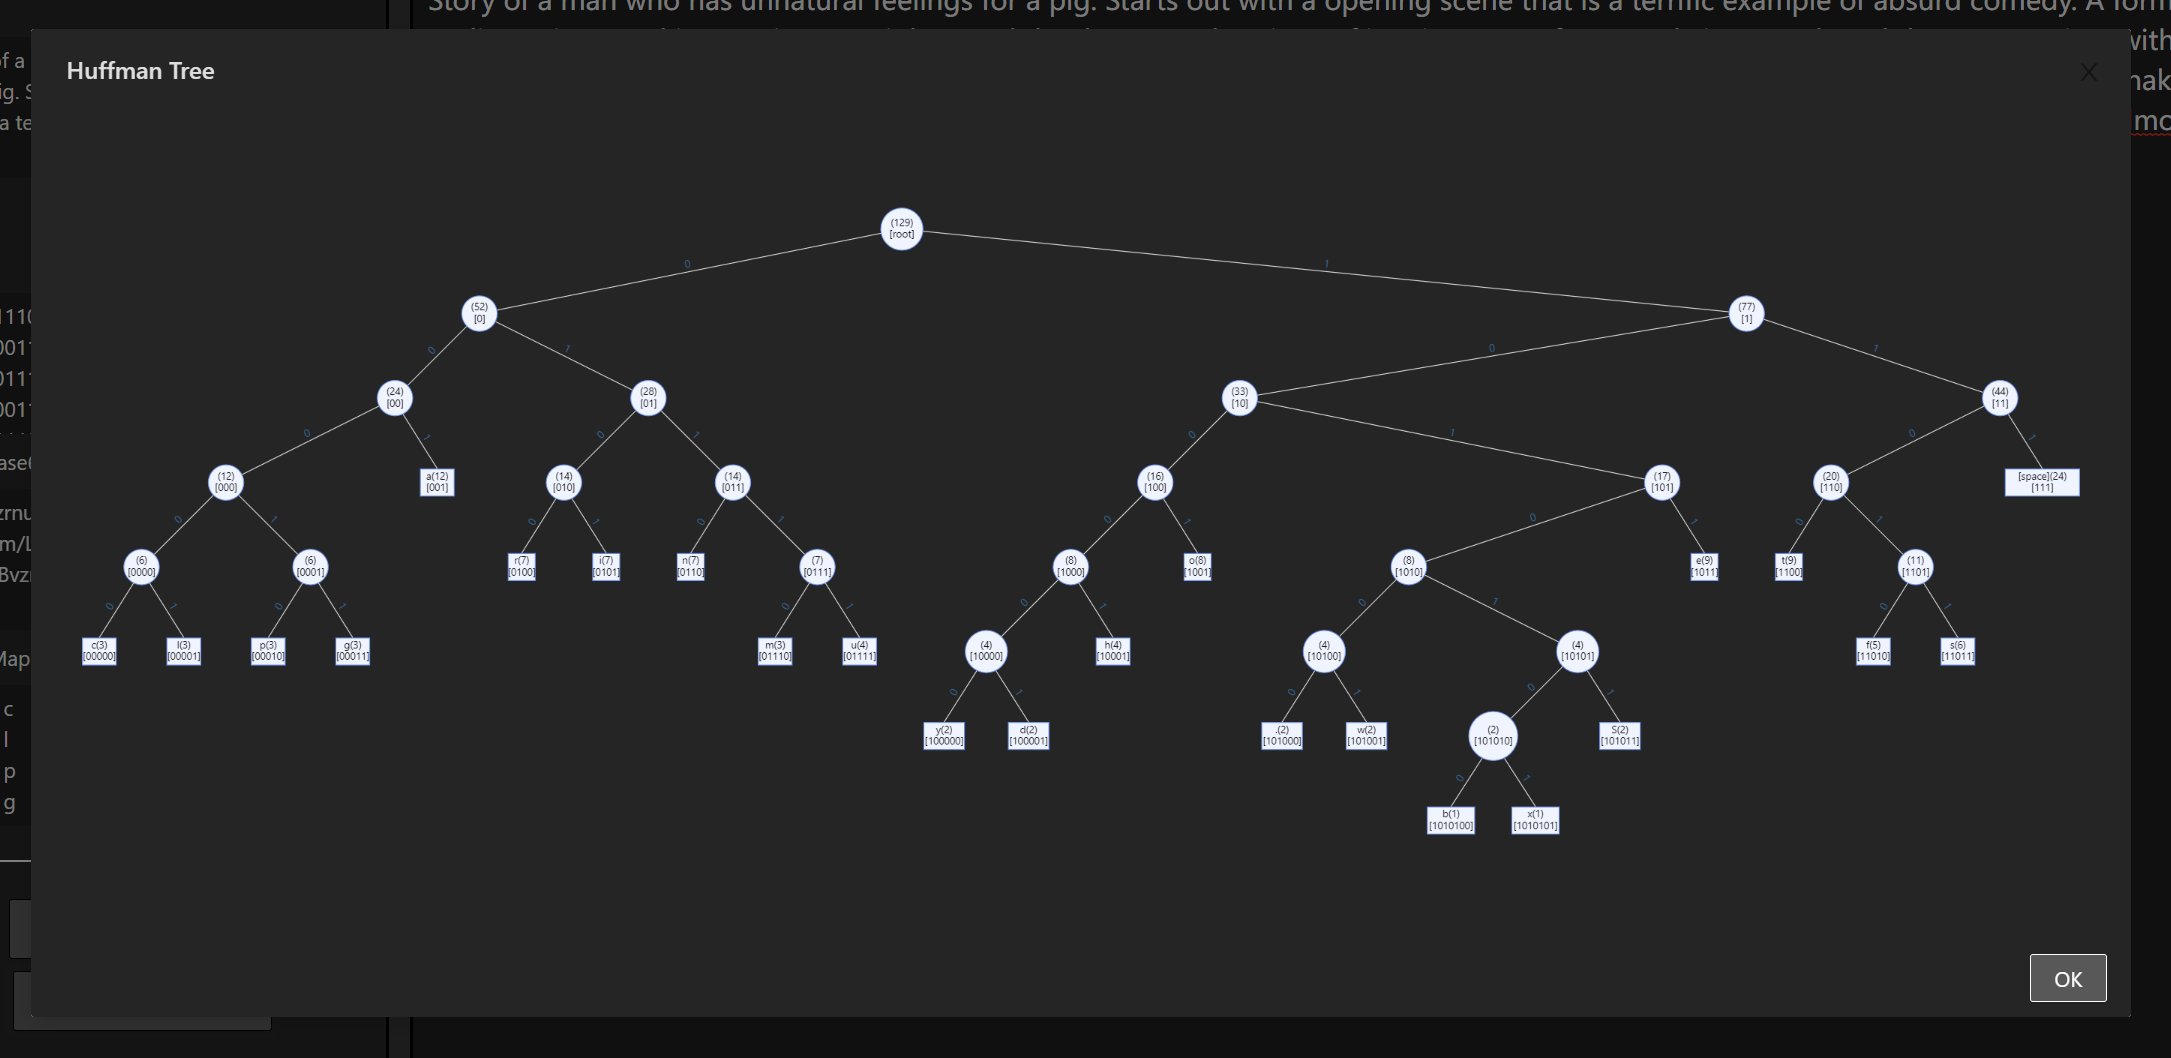
\includegraphics[width=\textwidth]{images/HuffmanTree-all.png}
    \caption{哈夫曼树可视化页内弹窗}
\end{figure}
\clearpage

\begin{figure}[h]
    \centering
    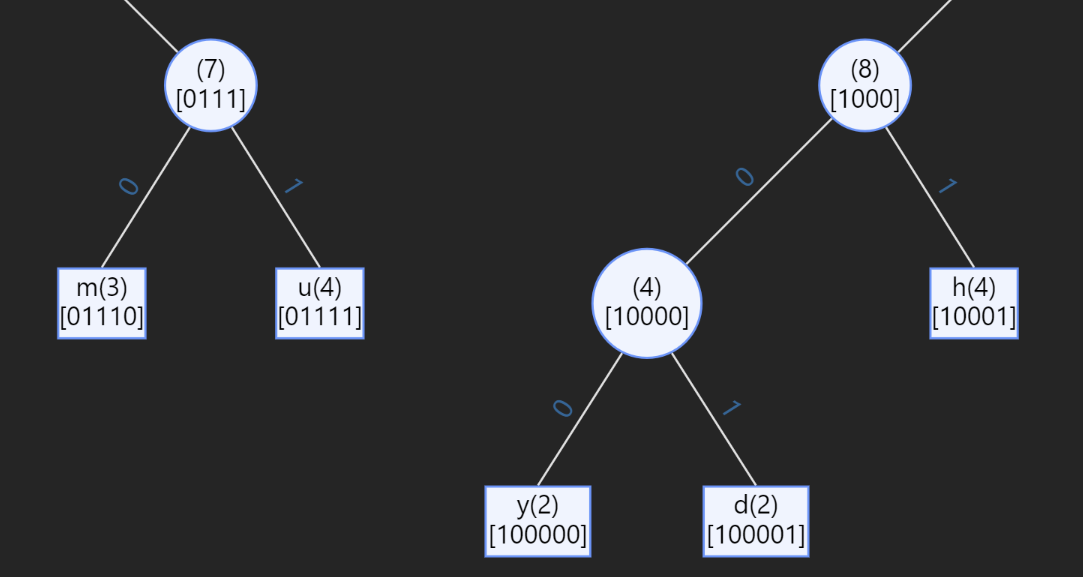
\includegraphics[width=0.6\textwidth]{images/HuffmanTree-part.png}
    \caption{哈夫曼树可视化局部}
\end{figure}

\begin{figure}[H]
    \centering
    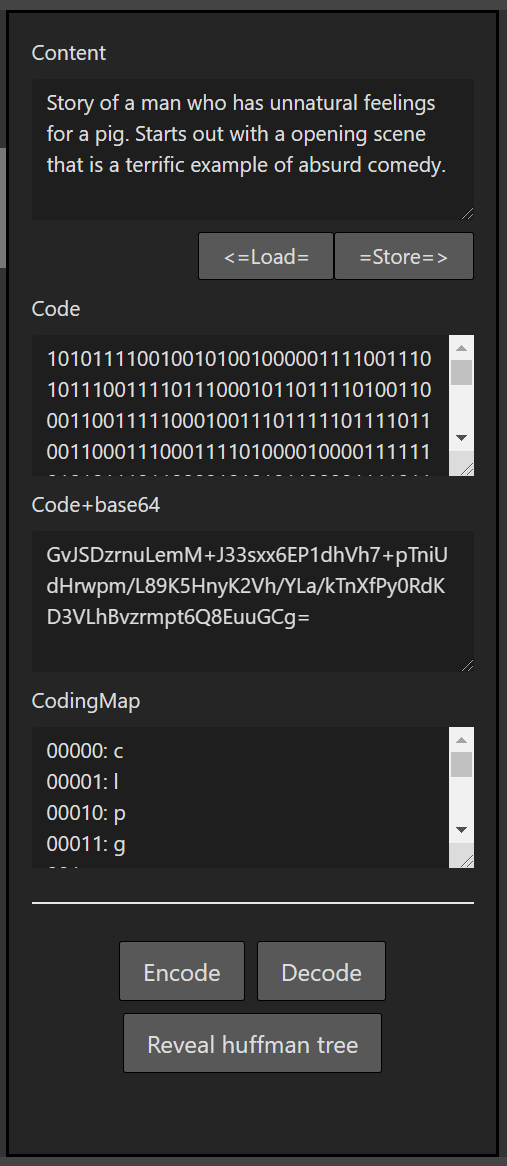
\includegraphics[width=0.5\textwidth]{images/EncodingPanel.png}
    \caption{编码译码侧栏}
\end{figure}
\clearpage

\subsubsection{查找替换侧栏FindAndReplace}

下图中展示了查找替换侧栏的两个状态,查找和替换状态。两个状态下的数据相互独立,可以在两个模式下随意切换,每个模式各自保留数据。

\paragraph{查找状态}
在当前打开的文件内检索指定内容,其功能如下:
\begin{itemize}
    \item 按下按钮后即会使用KMP算法进行匹配检索,并将结果列在下方
    \item 匹配的字符串会用黄底黑字高亮显示,同时自动解析前后若干个词(空格分隔)或达到指定最长字符数
    \item 上下按钮点击切换或直接点击某个结果,均可以自动在编辑器区域选中对应内容
\end{itemize}

\paragraph{替换状态}
在当前打开的文件内替换指定内容,其功能如下:
\begin{itemize}
    \item 同样使用KMP算法匹配,高亮并预览替换结果显示在下方
    \item 上下按钮点击切换或直接点击某个结果,均可以自动在编辑器区域选中对应内容
    \item 点击Replace按钮会替换当前文本,并自动使用替换后的文本长度变化,跳转到下一个替换处
    \item 点击Replace All按钮会替换掉所有可替换目标(仅会替换一次,如a替换为ab只会替换最初文本中的a,完成后会再次检索)
\end{itemize}

\begin{figure}[h]
    \centering
    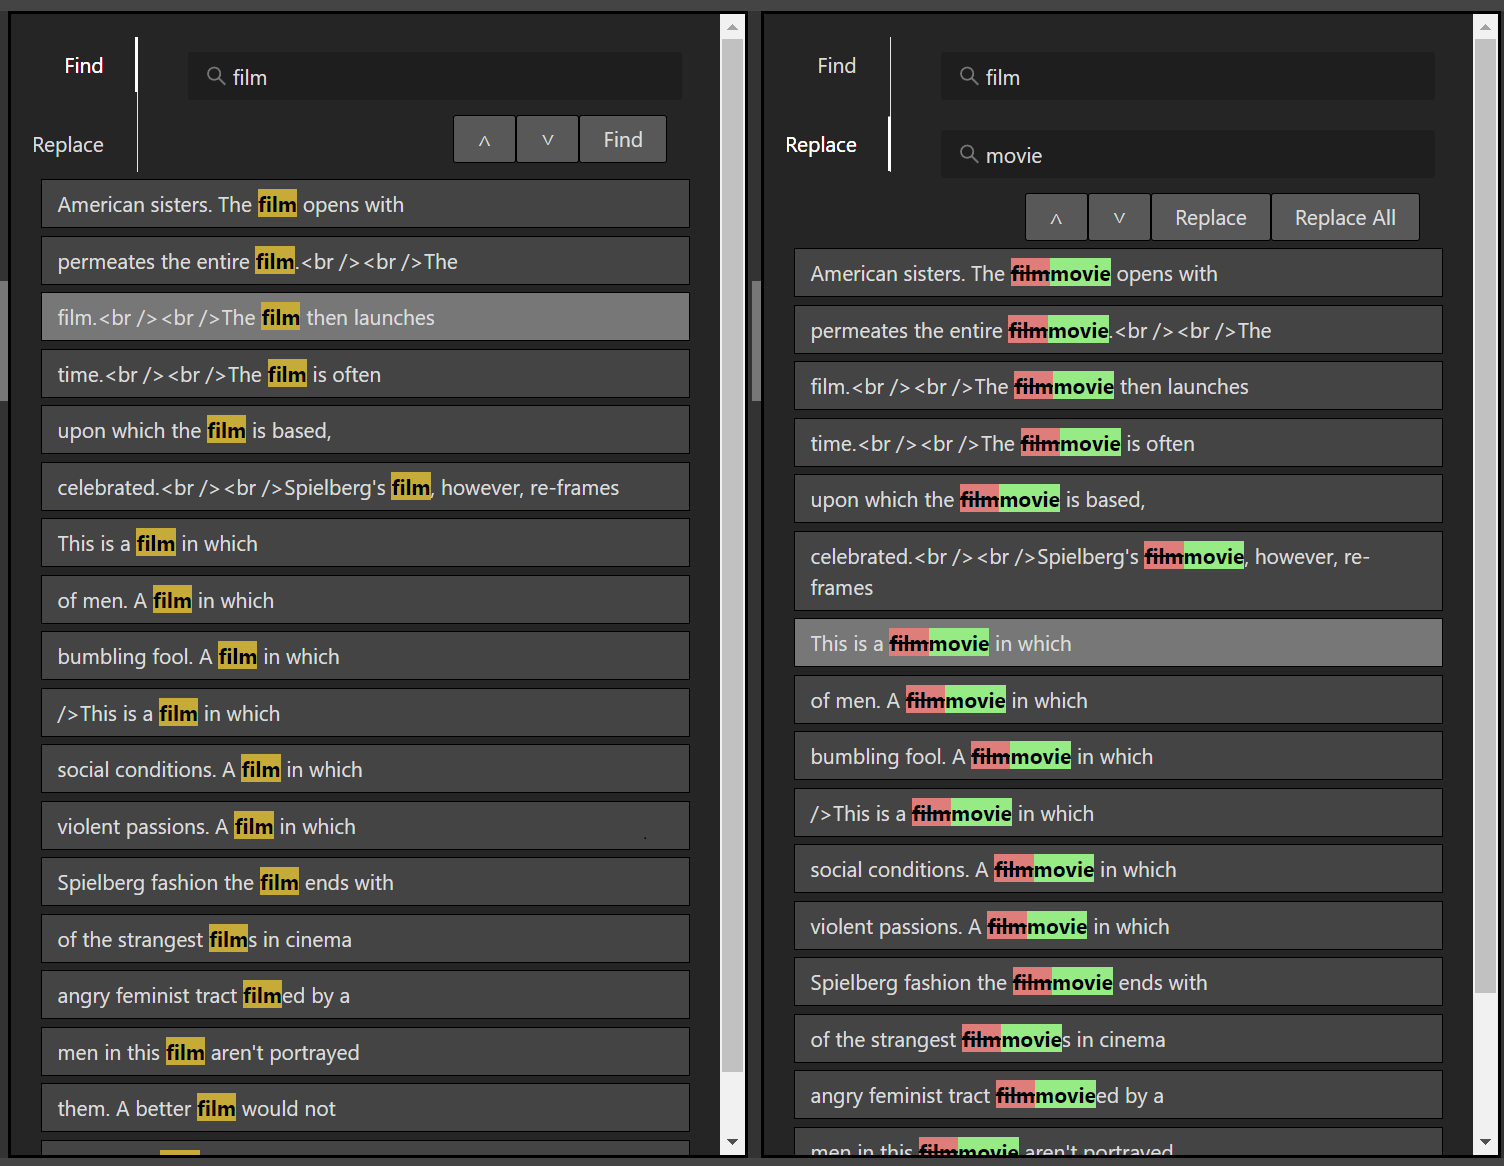
\includegraphics[width=\textwidth]{images/FindAndReplace.png}
    \caption{查找替换侧栏}
\end{figure}

\subsubsection{高级检索侧栏AdvancedSearch}
高级检索侧栏对目前工作区中所有文件(即最开始打开文件夹时扫描到的所有文件和后添加的文件)进行搜索。

当切换到此界面时,对工作区全部未索引文件进行索引,高级检索基于二级索引的结果,因此只有在索引全部完成后才能进行。

\paragraph{表达式检索}
在搜索框中输入检索表达式,点击搜索后会自动对表达式进行解析,根据集合运算找出匹配的文档,再根据TF-IDF权重进行相关性排序。最终显示到下方,每个文件显示各个匹配的位置,点击每条匹配词汇可以跳转到对应文件并自动选中对应位置。

\paragraph{同义词拓展}
当启用同义词非0时,系统会查询存储的同义词数据库,寻找指定数量的同义词,以或的方式加入到检索表达式中。每个关键词找到的同义词会被列在检索结果上方,同时附上IDF值。

\paragraph{选择显示数量}
用户可以选择显示的总文件数、单文件匹配位置数,实现自定义的显示效果。其中-1表示不限制,即显示所有的元素。

\begin{figure}[h]
    \centering
    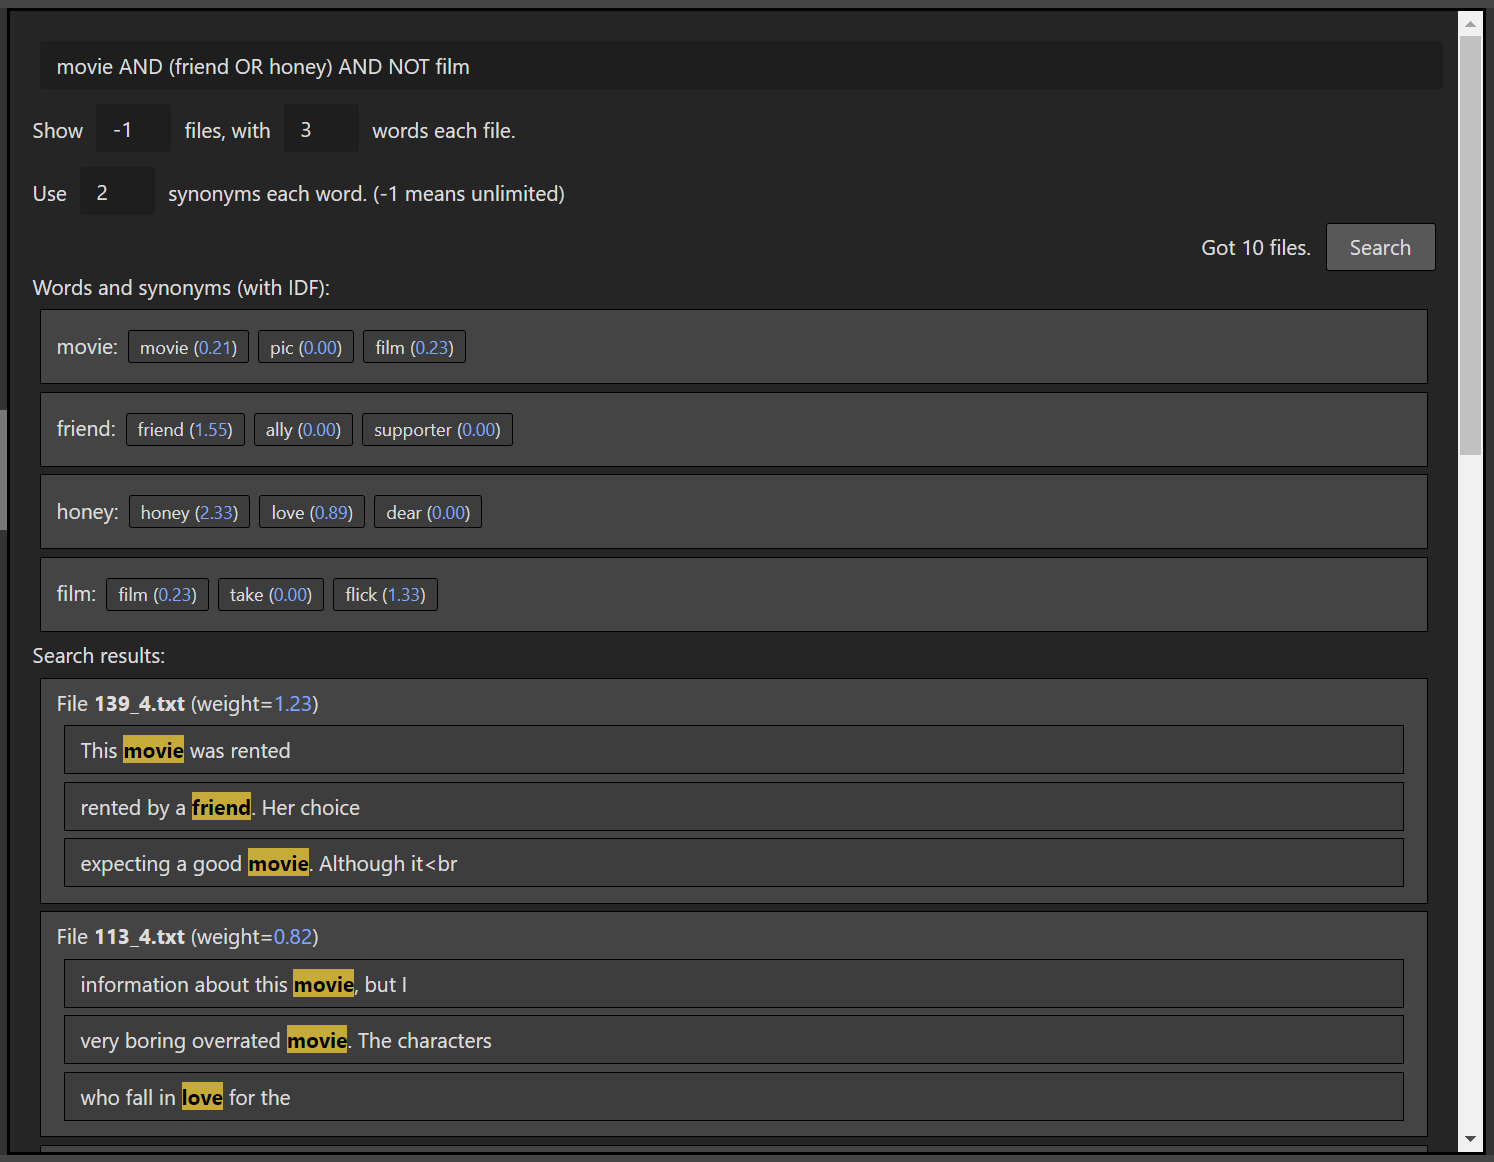
\includegraphics[width=\textwidth]{images/AdvancedSearch.png}
    \caption{高级检索侧栏}
\end{figure}

\clearpage

\subsubsection{词频侧栏Frequency}
词频侧栏对目前工作区中所有文件进行词频排序。

类似高级检索,当切换到此界面时,对工作区全部未索引文件进行索引。二级倒排索引会对词频进行统计,因此词频模块基本上就是将统计的结果显示出来。

\paragraph{三级显示层次}
词频统计分为三级显示,首先是按总词频统计对单词排序,然后每个词内部按文件词频对文件排序,最内部按词汇出现位置按先后排序。

\paragraph{选择显示数量}
用户可以选择显示的总词汇数、每个词汇显示的文件数、每个文件显示的匹配数。其中-1表示不限制,即显示所有的元素。


\begin{figure}[h]
    \centering
    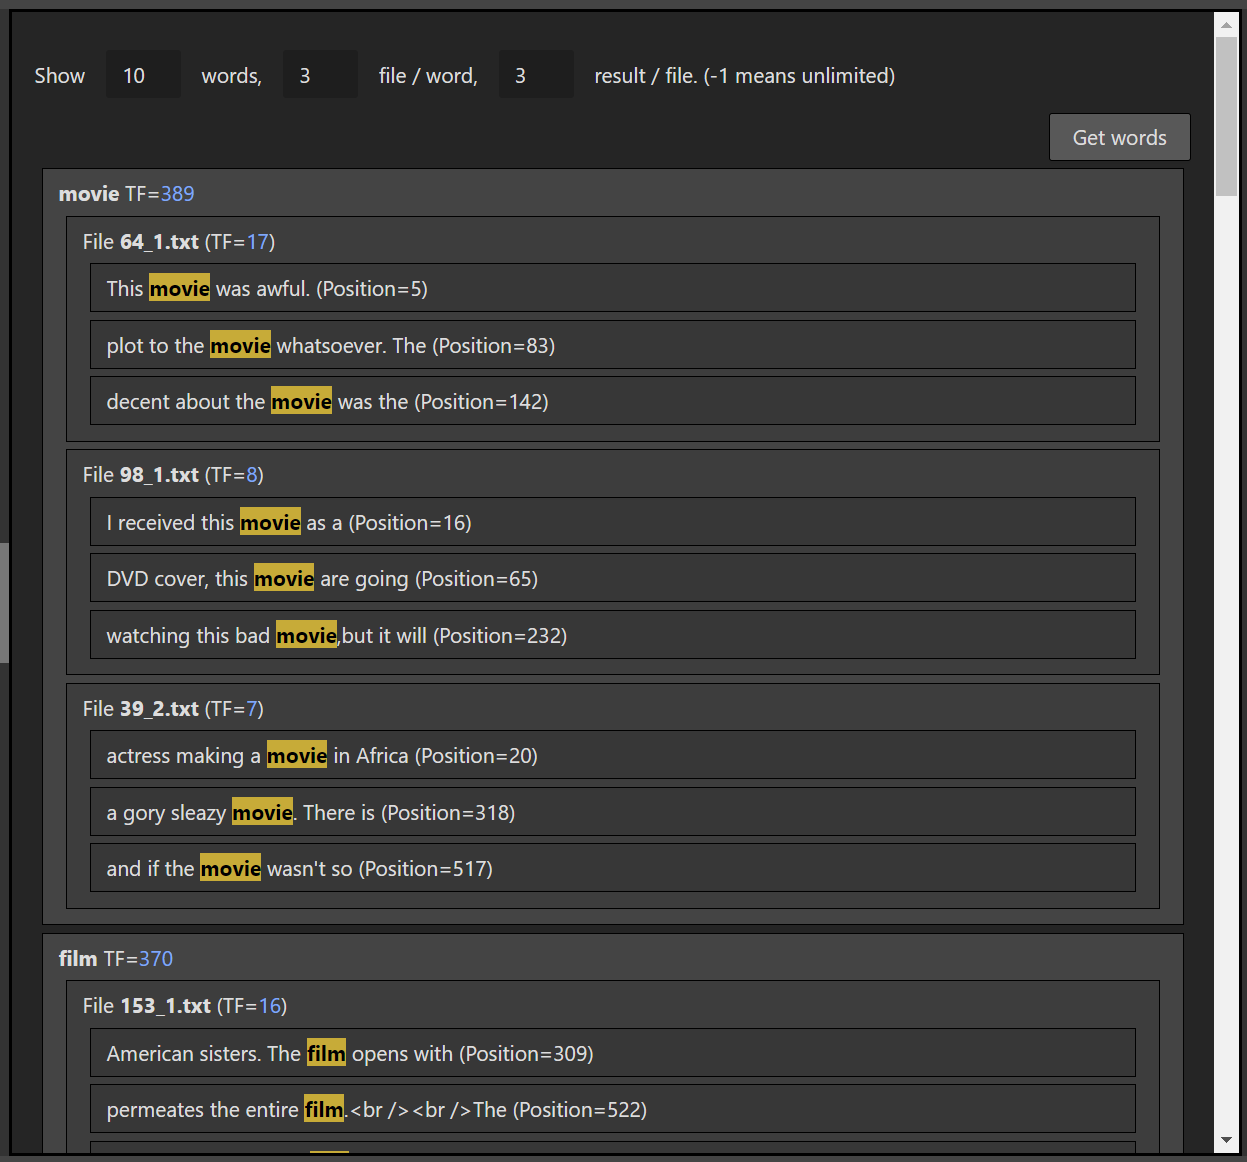
\includegraphics[width=\textwidth]{images/Frequency.png}
    \caption{词频侧栏}
\end{figure}

\clearpage

\section{详细设计}
详细设计中对主要的算法进行说明,包括数据结构的成员方法和独立的函数,较为次要的实现细节不再赘述。此外,给出系统整体和各部分的流程图,说明各部分直接的运行关系。

\subsection{KMP算法}
KMP算法依赖前缀函数实现字符串的匹配。这里重点说明前缀函数的求取算法,随后简单说明如何使用前缀函数匹配字符串。

\subsubsection{前缀函数}

\paragraph{前缀函数的定义} 任取长度为$n$的字符串$s$,其前缀函数为一个长度为$n$的数组$\pi$。其中$\pi[i]$等于子串$s[0\dots i]$的最长相等真前缀、真后缀的长度(其中,真前缀、真后缀指与原字符串不相等的前缀、后缀字符串)。
特别地,规定$\pi[0] = 0$。

用数学语言可描述如下:
$$
\begin{array}l
    \forall s, length(s) = n, \\
    \exists \pi[i] = \mathop{max}\limits_{0\leq k \leq i-1}\left( \left\{k+1| s[0\dots k] = s[i-k\dots i] \right\} \cup \left\{0\right\} \right), 0 \leq i \leq n \\
\end{array}
$$

\paragraph{求前缀函数} 思想主要包括以下几点:
\begin{outline}
    \1 从$\pi[1]$到$\pi[n]$逐一计算,前缀函数值每次最多增加$1$,分为增加一和其他两种情况
    \1 增加一:当$s[i+1]=s[\pi[i]]$时,$\pi[i+1] = \pi[i]+1$
    \1 其他:当$s[i+1]\ne s[\pi[i]]$时,我们寻找最大的$j\leq \pi[i]$,满足$s[0\dots j-1] = s[i-j+1\dots i]$
        \2 由$\pi[i]$的定义,有$s[0\dots \pi[i]-1] = s[i-\pi[i]+1\dots i]$
        \2 因为$j\leq \pi[i]$,$s[i-j+1\dots i]$是$s[i-\pi[i]+1\dots i]$的子串
        \2 故两等式联合有$s[0\dots j-1] = s[i-j+1\dots i] = s[\pi[i]-j\dots \pi[i]-1]$
        \2 根据$\pi$的定义,由上式可知$j=\pi[\pi[i]-1]$
\end{outline}

以上算法中“其他”情况下可以直观地参照下式理解:
\begin{outline}
    \1 首先,已知两个$\pi[i]$长的字符串(上方大括号)相等,可以知道(从左到右数)第2个和第3个标记出的长度为$j$的字符串相等
    \1 随后,要求第1个和第3个长度为$j$的字符串相等,就等价于要求第1个和第2个长度为$j$的字符串相等,即是求$\pi[\pi[i]-1]$时的要求
\end{outline}
$$ \overbrace{\underbrace{s_0 ~ s_1}_j ~ s_2 ~ s_3 ~ \underbrace{s_4 ~ s_5}_j}^{\pi[i]} ~ \dots ~ \overbrace{s_{i-5} ~ s_{i-4} ~ s_{i-3} ~ s_{i-2} ~ \underbrace{s_{i-1} ~ s_{i}}_j}^{\pi[i]} ~ s_{i+1} $$

\clearpage

求解前缀函数算法的伪代码如下:
\begin{algorithm}[H]
    % \renewcommand{\linespread}{1}
    % \setstretch{1}
    \caption{求前缀函数}
    \begin{algorithmic}[1]
        \Require{A string s}
        \Ensure{The prefix array $\pi$}
        \Procedure{PrefixFunction}{$s$}
            \State $\pi$ \gets [~]
            \State $\pi$.\textsc{PushBack}(0)
            \For{i in 0 to \textsc{Length}(s)}
                \State j \gets $\pi$[i-1]
                \While{j > 0 \textbf{and} $\pi[i] \neq \pi[j]$}
                    j = $\pi[j - 1]$
                \EndWhile
                \If{$s[i] = s[j]$}
                    \State $\pi.\textsc{PushBack}(j+1)$
                \Else
                    \State $\pi.\textsc{PushBack}(0)$
                \EndIf
            \EndFor
        \EndProcedure
    \end{algorithmic}
\end{algorithm}

\subsubsection{使用前缀函数匹配字符串}
使用前缀函数求解算法可以轻易地匹配字符串。

首先,拼接出形如$Target~\phi~Content$的字符串,其中$Target$是搜索目标,$Content$是检索的原文,而$\phi$是二者中都不可能出现的特殊字符。

其次,对拼接出的字符串求前缀函数,当出现$i>length(Target)$且$\pi[i] = length(Target)$的时候,意味着在$Content$中$i-2\times length(Target) - 1$的位置出现了$Target$。

\subsection{闭散列}
我将功能划分为散列函数$h()$、探查函数$p()$、闭散列框架三部分。其中前两者可根据需求进行替换。这样实现了高自由度的闭散列功能。

\subsubsection{闭散列框架}
闭散列框架的核心功能是查找函数$find()$。它可以借助散列函数$h()$、探查函数$p()$,来探查目标元素,并返回探查的结果(找到、目标为空或查找次数过多)和目标元素的位置。其他功能调用查找函数$find()$实现功能。

\paragraph{查找函数$find()$} 本质上是一个有最多次数限制的探查循环。从哈希码开始,每次循环后用哈希码、探查次数、目标元素通过探查函数$p()$获取下一个探查位置。其伪代码如下:

\begin{algorithm}[H]
    \caption{查找函数$find()$}
    \begin{algorithmic}[1]
        \Require{Target Element e}
        \Ensure{Result, position of e}
        \Function{find}{$e$}
            \State d0 \gets \textsc{h}(e)
            \State d \gets d0
            \For{i in 1 to MaxTryTimes}
                \If{$array[d] = e$}
                    \State \Return FOUND, d
                \ElsIf{$array[d] = NULL$}
                    \State \Return EMPTY, d
                \EndIf
                \State d \gets (d0 + \textsc{p}(i, e) \textbf{mod} capacity + capacity) \textbf{mod} capacity
            \EndFor
            \State \Return TIMES\_EXCEED, d
        \EndFunction
    \end{algorithmic}
\end{algorithm}

\paragraph{对外提供功能} 闭散列基于查找函数$find()$对外提供了增加元素、查找元素、删除元素和列出现有所有元素的功能。

其中,前三者均会使用提供的字符串调用$find()$,然后对结果和位置$d$进行不同的处理。具体如下:
\begin{table}[H]
    \centering
    \caption{添加、查找、删除元素功能实现}
    \begin{tabular}{cccc}
        \toprule
        功能名称 & 返回$FOUND$ & 返回$EMPTY$ & 返回$TIMES\_EXCEED$ \\
        \midrule
        添加元素 & 返回$d$ & \makecell[c]{
            设置$array[d]$为新元素 \\
            返回$d$ \\
        } & 返回$NULL$ \\
        \midrule
        查找元素 & 返回$d$ & 返回$NULL$ & 返回$NULL$ \\
        \midrule
        删除元素 & \makecell[c]{
            设置$array[d]$为墓碑 \\
            返回 \\
        } & 返回 & 返回 \\
        \bottomrule
    \end{tabular}
\end{table}

而列出现有所有元素的功能只需要遍历$array$即可实现。

\paragraph{构造函数} 构造闭散列表时可以设定容量、最大检索次数和探查函数$p()$。由于课设中所有散列表均针对字符串使用,因此固定了散列函数$h()$。

\subsubsection{散列函数h()}
由于结果不需要用于密码学相关用途,对字符串的散列只需要保证字符串的每位均会对结果产生较显著的影响即可。为此我采用Stack Overflow上经过讨论认为速度较快的算法。

主要思想是先将字符串变为字符数组,再逐一对字符的ASCII码进行$result \gets result \times 31 + new$的迭代运算。伪代码如下:
\begin{algorithm}[H]
    \caption{散列函数$h()$}
    \begin{algorithmic}[1]
        \Require{A string s}
        \Ensure{Hash code of s}
        \Function{find}{$s$}
            \State hash \gets 0
            \For{i in 1 to \textsc{Length}(s)}
                \State hash \gets (hash << 5) - hash + \textsc{ASCII}(s[i])
            \EndFor
            \State \Return hash
        \EndFunction
    \end{algorithmic}
\end{algorithm}

\subsubsection{探查函数p()}
实践中发现,由于默认使用的闭散列容量较大,且字符串的哈希码不太容易出现碰撞,较为简单的线性探查、二次探查就已经足够使用。

\paragraph{线性探查} 单向逐一探查,公式如下:
$$
p(i, e) = i
$$

\paragraph{二次探查} 越来越远地双向探查,公式如下:
$$
p(i, e) = (-1)^{i+1} \times \ceil*{\frac{i}{2}}^2
$$

\subsection{二级倒排索引}

\subsubsection{整体设计}
二级倒排索引的目的是对多文档中词出现的频率、位置进行索引,并当部分文档变化时高效更新。具体设计如下:
\begin{outline}
    \1 一级索引为文件索引(FileIndex类)
        \2 对单文件的内容索引,记录每个词出现的所有位置
        \2 对于每个词,出现位置的个数即是词频
        \2 只读。本质上是对文本内容索引,当出现新文档或文档内容变更时(用户修改并移开焦点或搜索替换后)重新进行索引
    \1 二级索引为全局索引(WorkspaceIndex类)
        \2 对文件索引进行索引,记录每个词在不同出现的所有文件和数量
        \2 对于每个词,维护出现它的文件索引的引用和总出现次数
        \2 记录当前包含的所有文件索引,仅需在新增或移除文件索引时更新
\end{outline}

注:这里提到的“词”指标准化处理后的词,系统会首先对文本中提取的每个词进行去停用词、转小写等操作。

\subsubsection{数据结构设计}

\paragraph{文件索引} 包含以下内容:
\begin{table}[H]
    \centering
    \caption{文件索引存储内容}
    \begin{tabular}{ccc}
        \toprule
        名称 & 类型 & 含义 \\
        \midrule
        词位置索引 & 对应表:字符串\rightarrow 数组 & 词\rightarrow 出现的所有位置 \\
        哈希值 & 数值 & 索引内容的哈希码,唯一标识文件索引 \\
        索引的文件结点 & 文件结点 & 用于提取内容等操作 \\
        \bottomrule
    \end{tabular}
\end{table}

\paragraph{全局索引} 包含以下内容:
\begin{table}[H]
    \centering
    \caption{全局索引存储内容}
    \begin{tabular}{ccc}
        \toprule
        名称 & 类型 & 用途 \\
        \midrule
        词索引 & 对应表:字符串\rightarrow 文件索引组和总词频 & 词\rightarrow 出现的文件和总词频 \\
        全部文件索引的索引 & 对应表:数值\rightarrow 文件索引 & 文件索引哈希值\rightarrow 文件索引 \\
        \bottomrule
    \end{tabular}
\end{table}

\subsubsection{算法设计}

\paragraph{文件索引} 文件索引是只读的,因此只需要每次根据内容构造以及查询词汇。

\subparagraph{-~根据内容构造}首先对内容按空格分割,对每个词进行标准化,随后不断从对应表中获取并添加位置。

\subparagraph{-~查询词汇}使用对应表的查询功能,返回所有位置的数组,对数组取长度可以得到词频。

\paragraph{全局索引} 全局索引需要维护当前包含的文件索引,还要实现全局的查询词汇。

\subparagraph{-~维护当前包含的索引} 即需要实现添加、删除索引。

全部文件索引的索引用于保证此操作合法。

需要对新添加或删除索引中的每个词,对应地在全局索引中进行处理,在对应词中新增或删除这个文件索引,并维护总词频。

\subparagraph{-~全局查询词汇} 调用词索引中的查询功能即可,可以查询出现的各个文件,进而查询出现的各个位置;也可以快速地运用总词频排序。

\clearpage

\subsection{相关性评价}
在进行多文档的相关性检索时,需要对根据检索表达式对文档进行相关性排序。而排序的依据是相关性评价的值。

\paragraph{表达式解析} 
表达式由关键词、括号和\emph{AND}、\emph{OR}、\emph{NOT}三种运算符组成。

由于表达式解析只支持二元运算符,我将所有的\emph{NOT}~X转换为\emph{ALL}~\emph{SUB}~X。

在开启近义词扩展时,我会将每个关键词$X$变为其近义词$X_1, X_2, \dots$的或表达式。如$X \rightarrow (X~\textbf{OR}~X_1~\textbf{OR}~X_2~\textbf{OR}~\dots)$。

随后使用一个存放括号和运算符的栈即可将中缀表达式转换为后缀表达式。后缀表达式中没有括号,可以便捷地进行计算,表达式解析完成。

\paragraph{集合运算:文档范围筛选} 对表达式进行集合运算,以此筛选出符合要求的文档。

每个关键词被它出现过的文档集合代替,\emph{ALL}对应全集。其中集合使用我基于闭散列实现的集合类$HashSet$对象。

运算\emph{AND}、\emph{OR}和\emph{SUB}则分别对应集合的交、并、补运算。

\paragraph{权重运算:相关性数值} 对表达式进行权重运算,以此计算出相关性数值用于排序。

每个关键词被它在该文档中出现的次数代替,\emph{ALL}赋予一个很大的常数。

运算\emph{AND}、\emph{OR}和\emph{SUB}则分别对应数值的最小值、最大值、减运算。

\paragraph{整体流程} 进行相关性检索式,首先解析表达式,然后用集合运算筛选出符合条件的文档,最后用权重运算为符合条件的文档计算相关值,按相关值排序显示在搜索结果中。

\subsection{流程图}

\subsubsection{整体流程图}
系统的整体流程图如下所示,各部分流程图分别说明各步骤更细致的流程。

\begin{figure}[h]
    \centering
    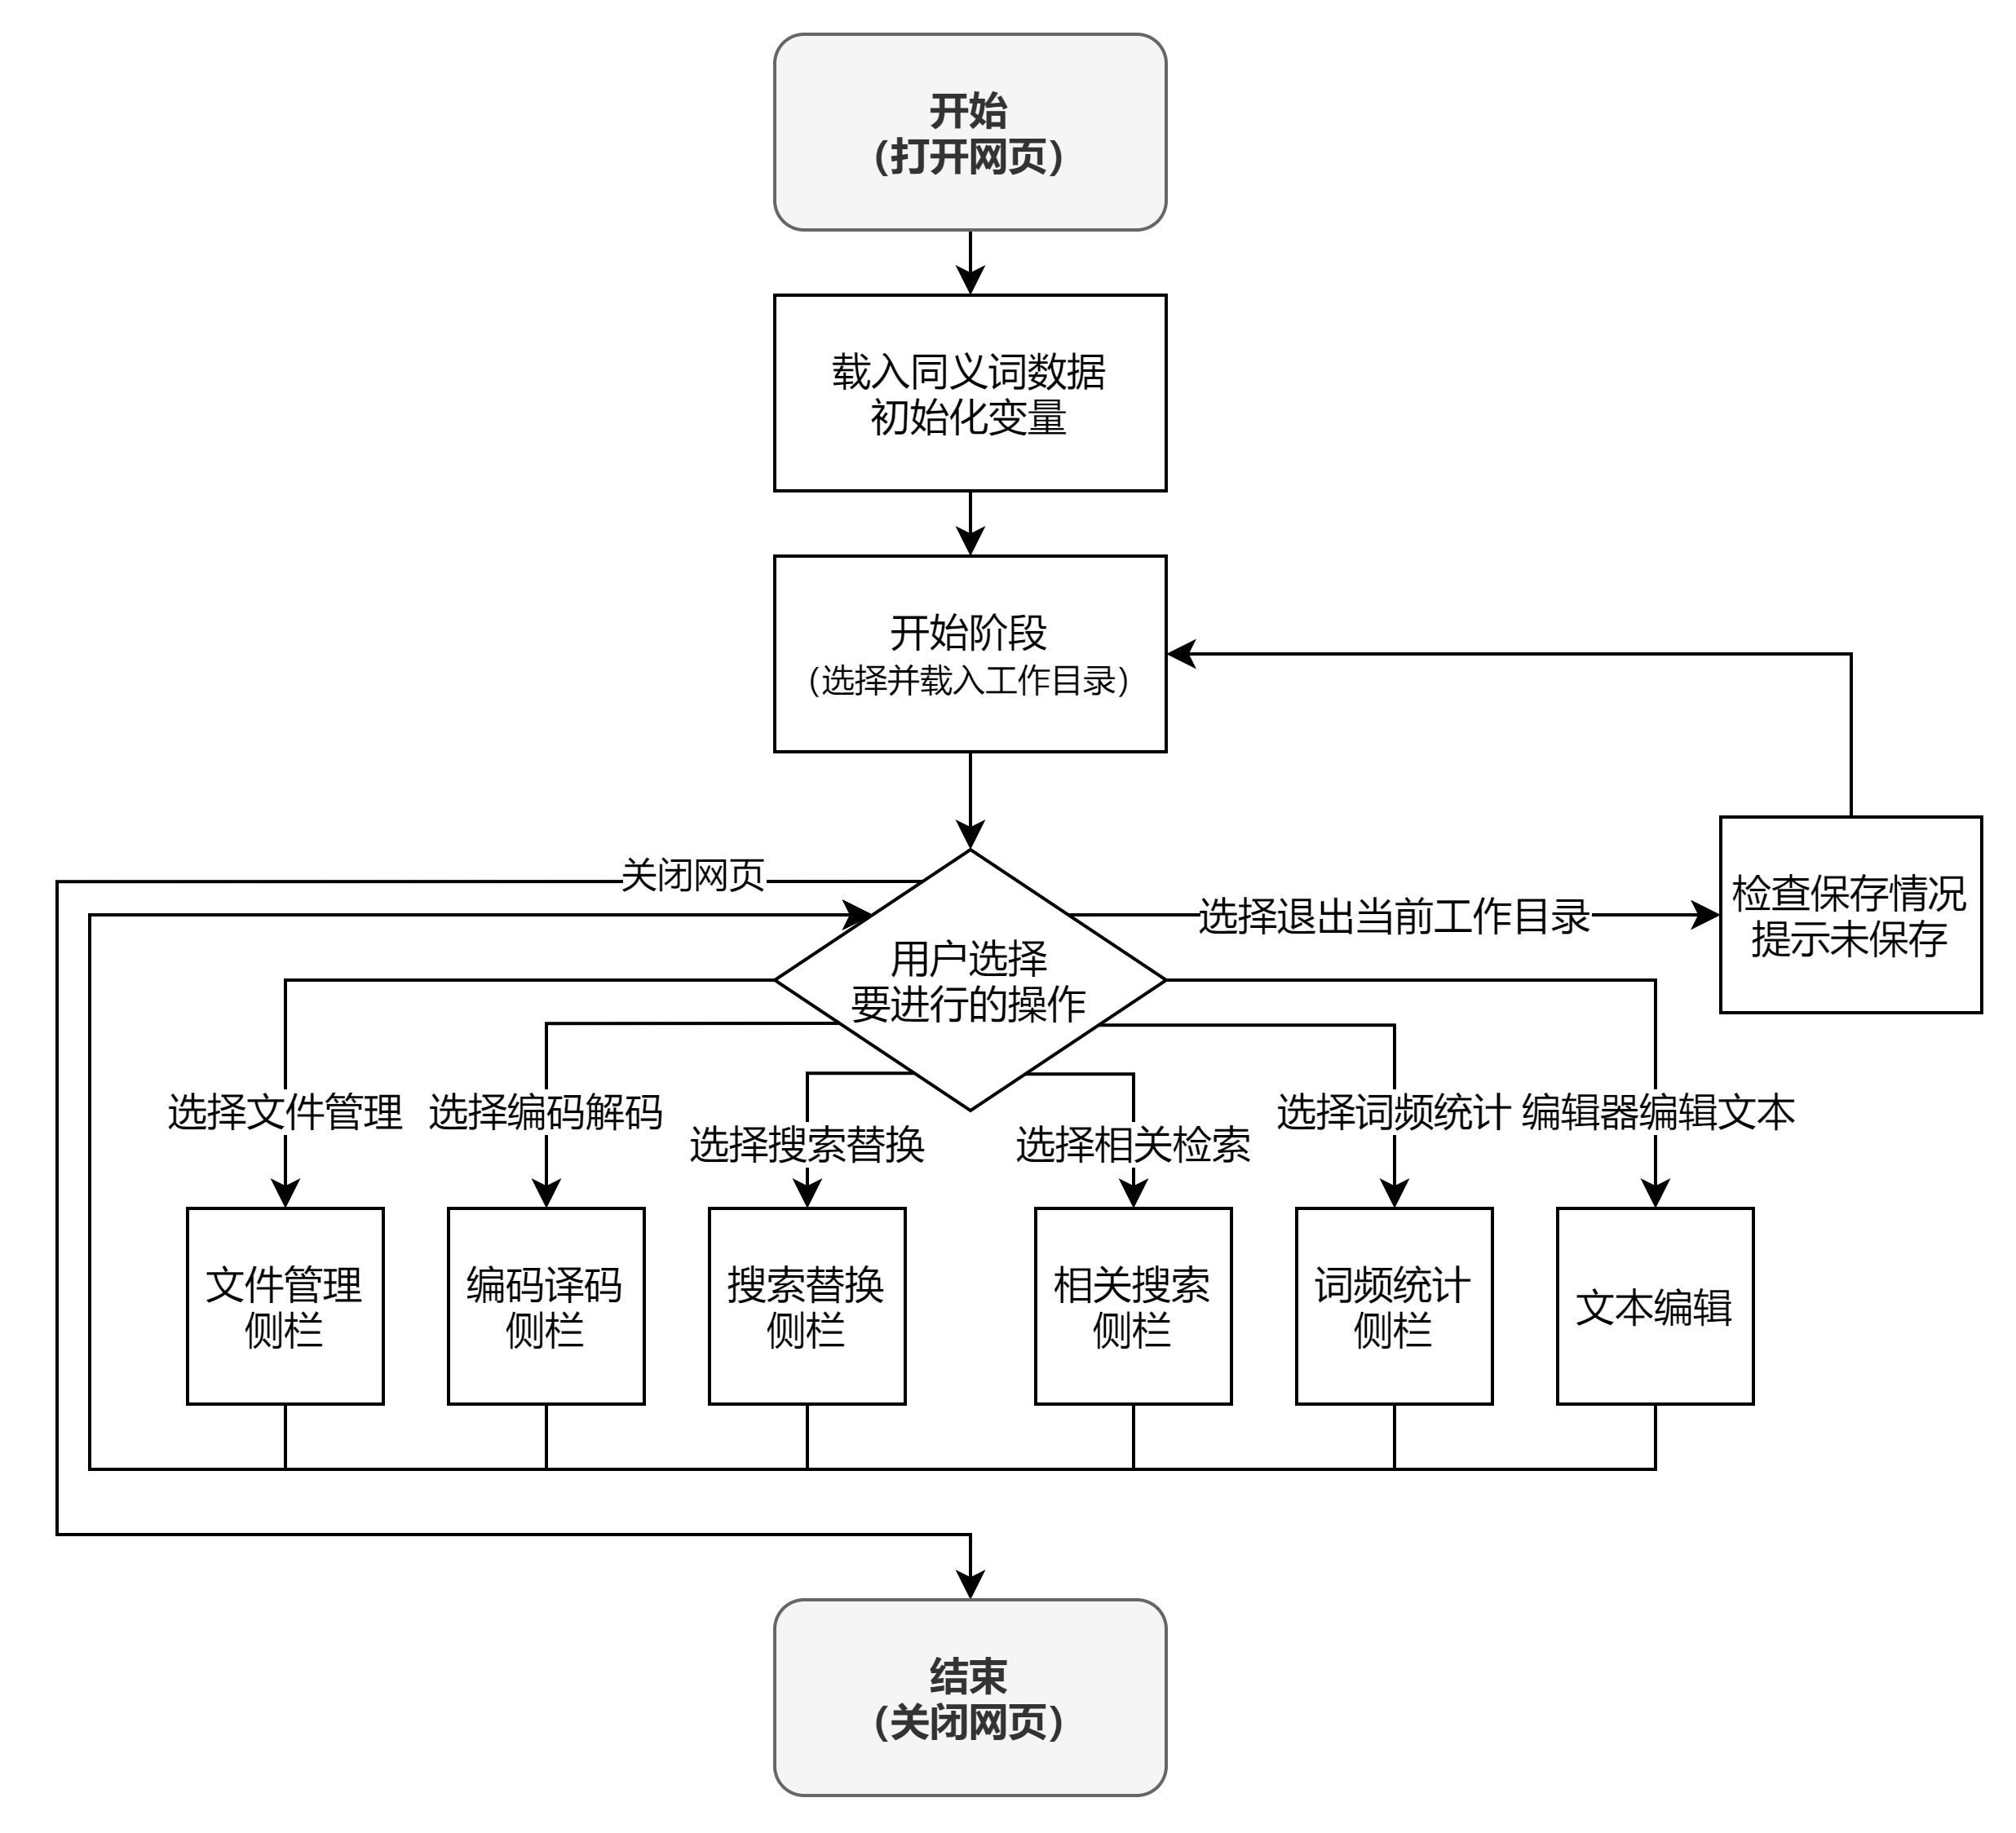
\includegraphics[width=0.8\textwidth]{images/dsacd-总流程图.drawio.png}
    \caption{整体流程图}
\end{figure}

\begin{figure}[h]
    \centering
    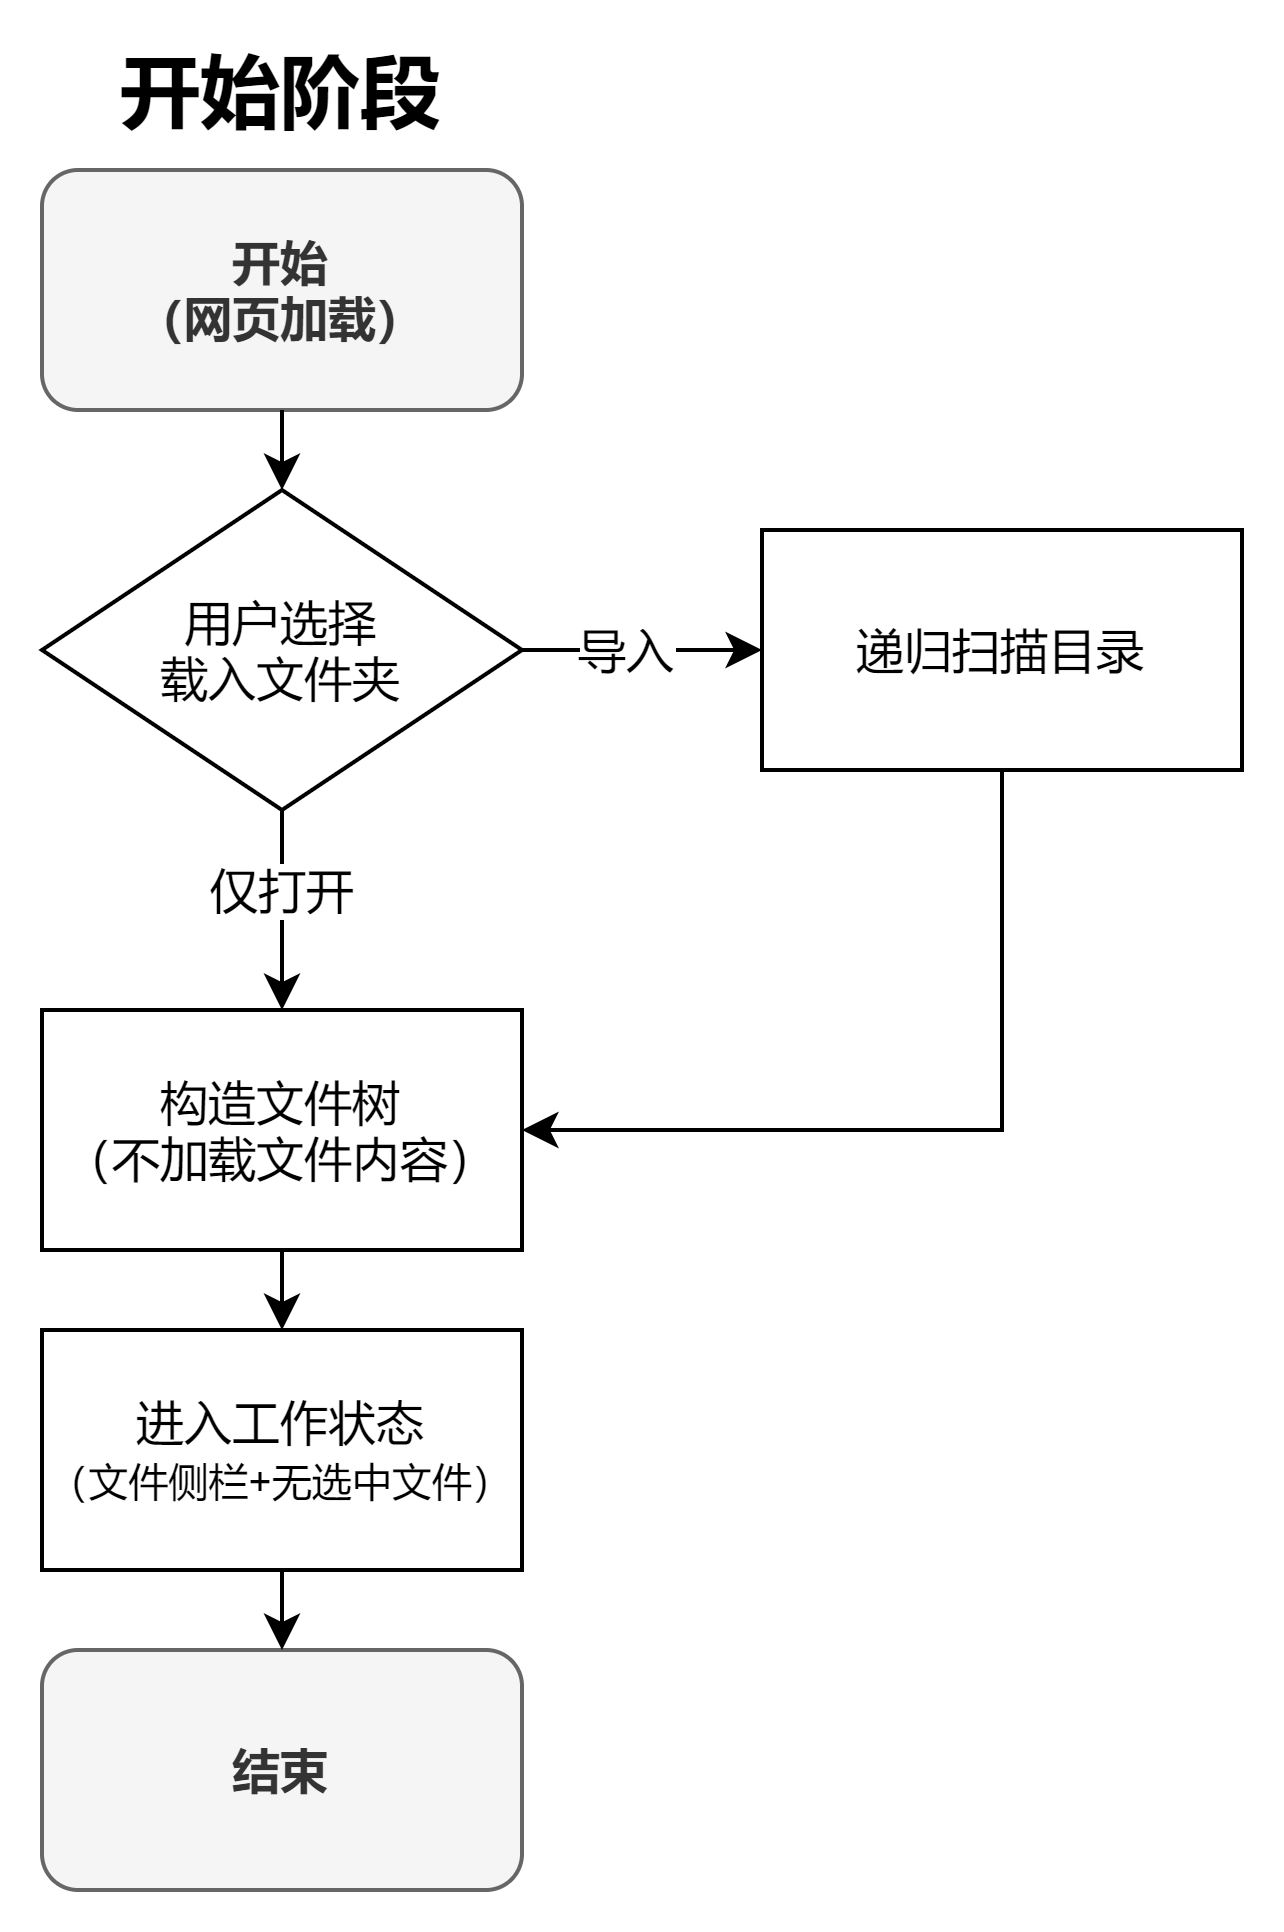
\includegraphics[width=0.4\textwidth]{images/dsacd-流程图-开始阶段.drawio.png}
    \caption{开始阶段流程图}
\end{figure}

\begin{figure}[h]
    \centering
    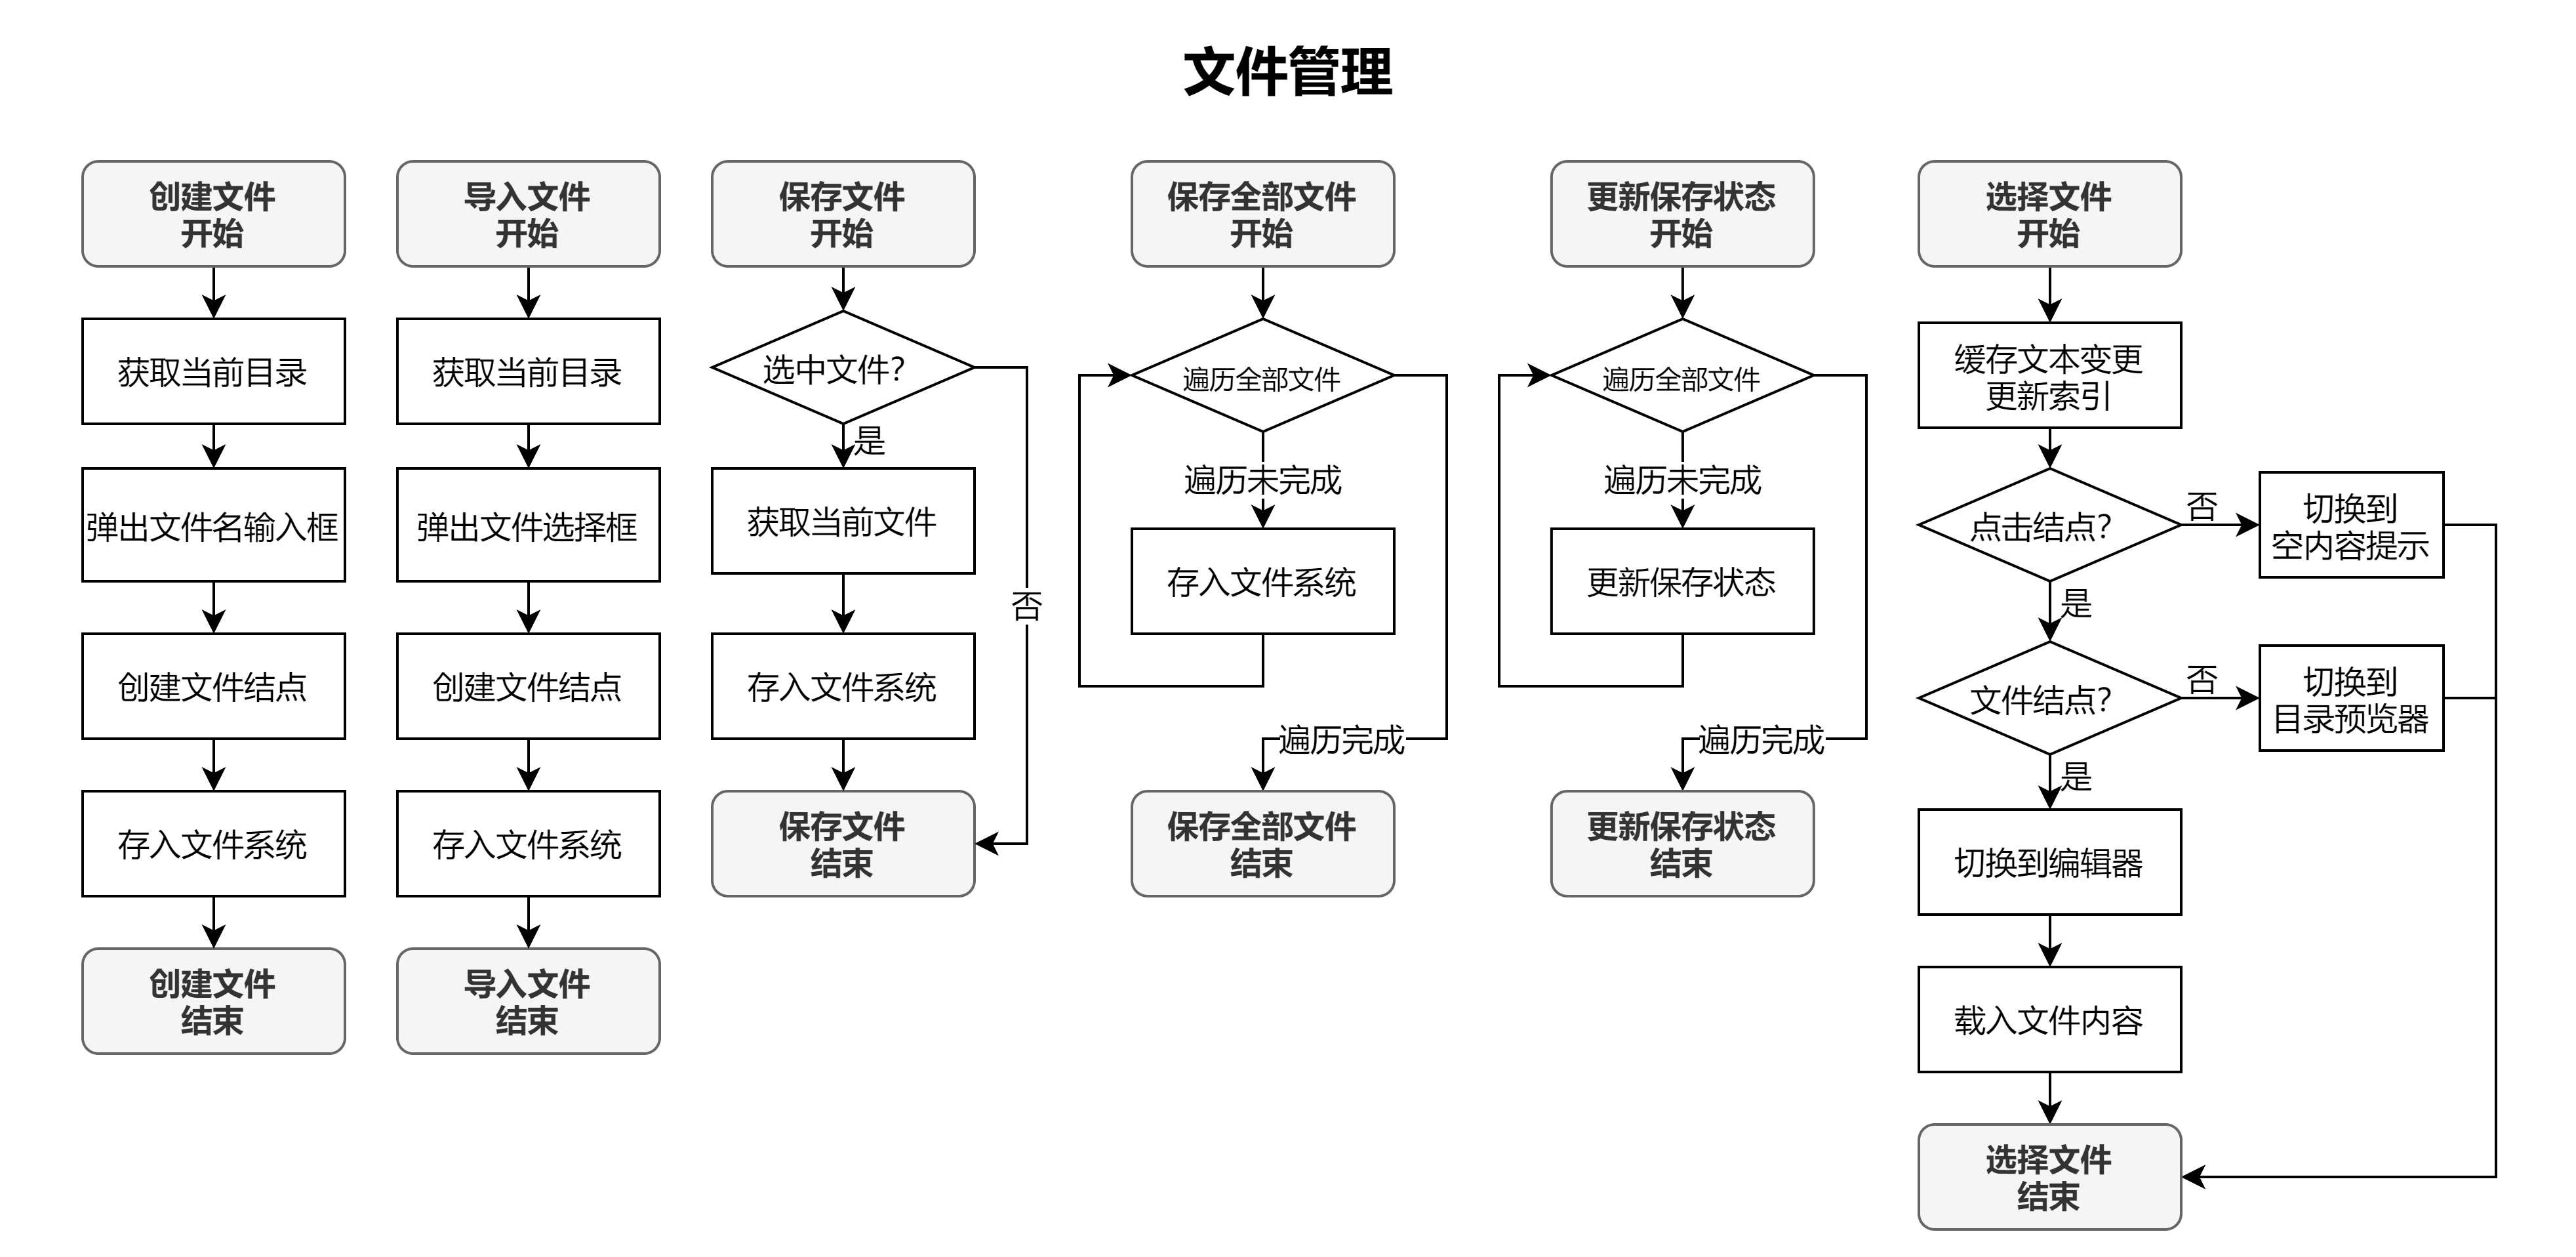
\includegraphics[width=\textwidth]{images/dsacd-流程图-文件管理.drawio.png}
    \caption{文件管理流程图}
\end{figure}

\begin{figure}[h]
    \centering
    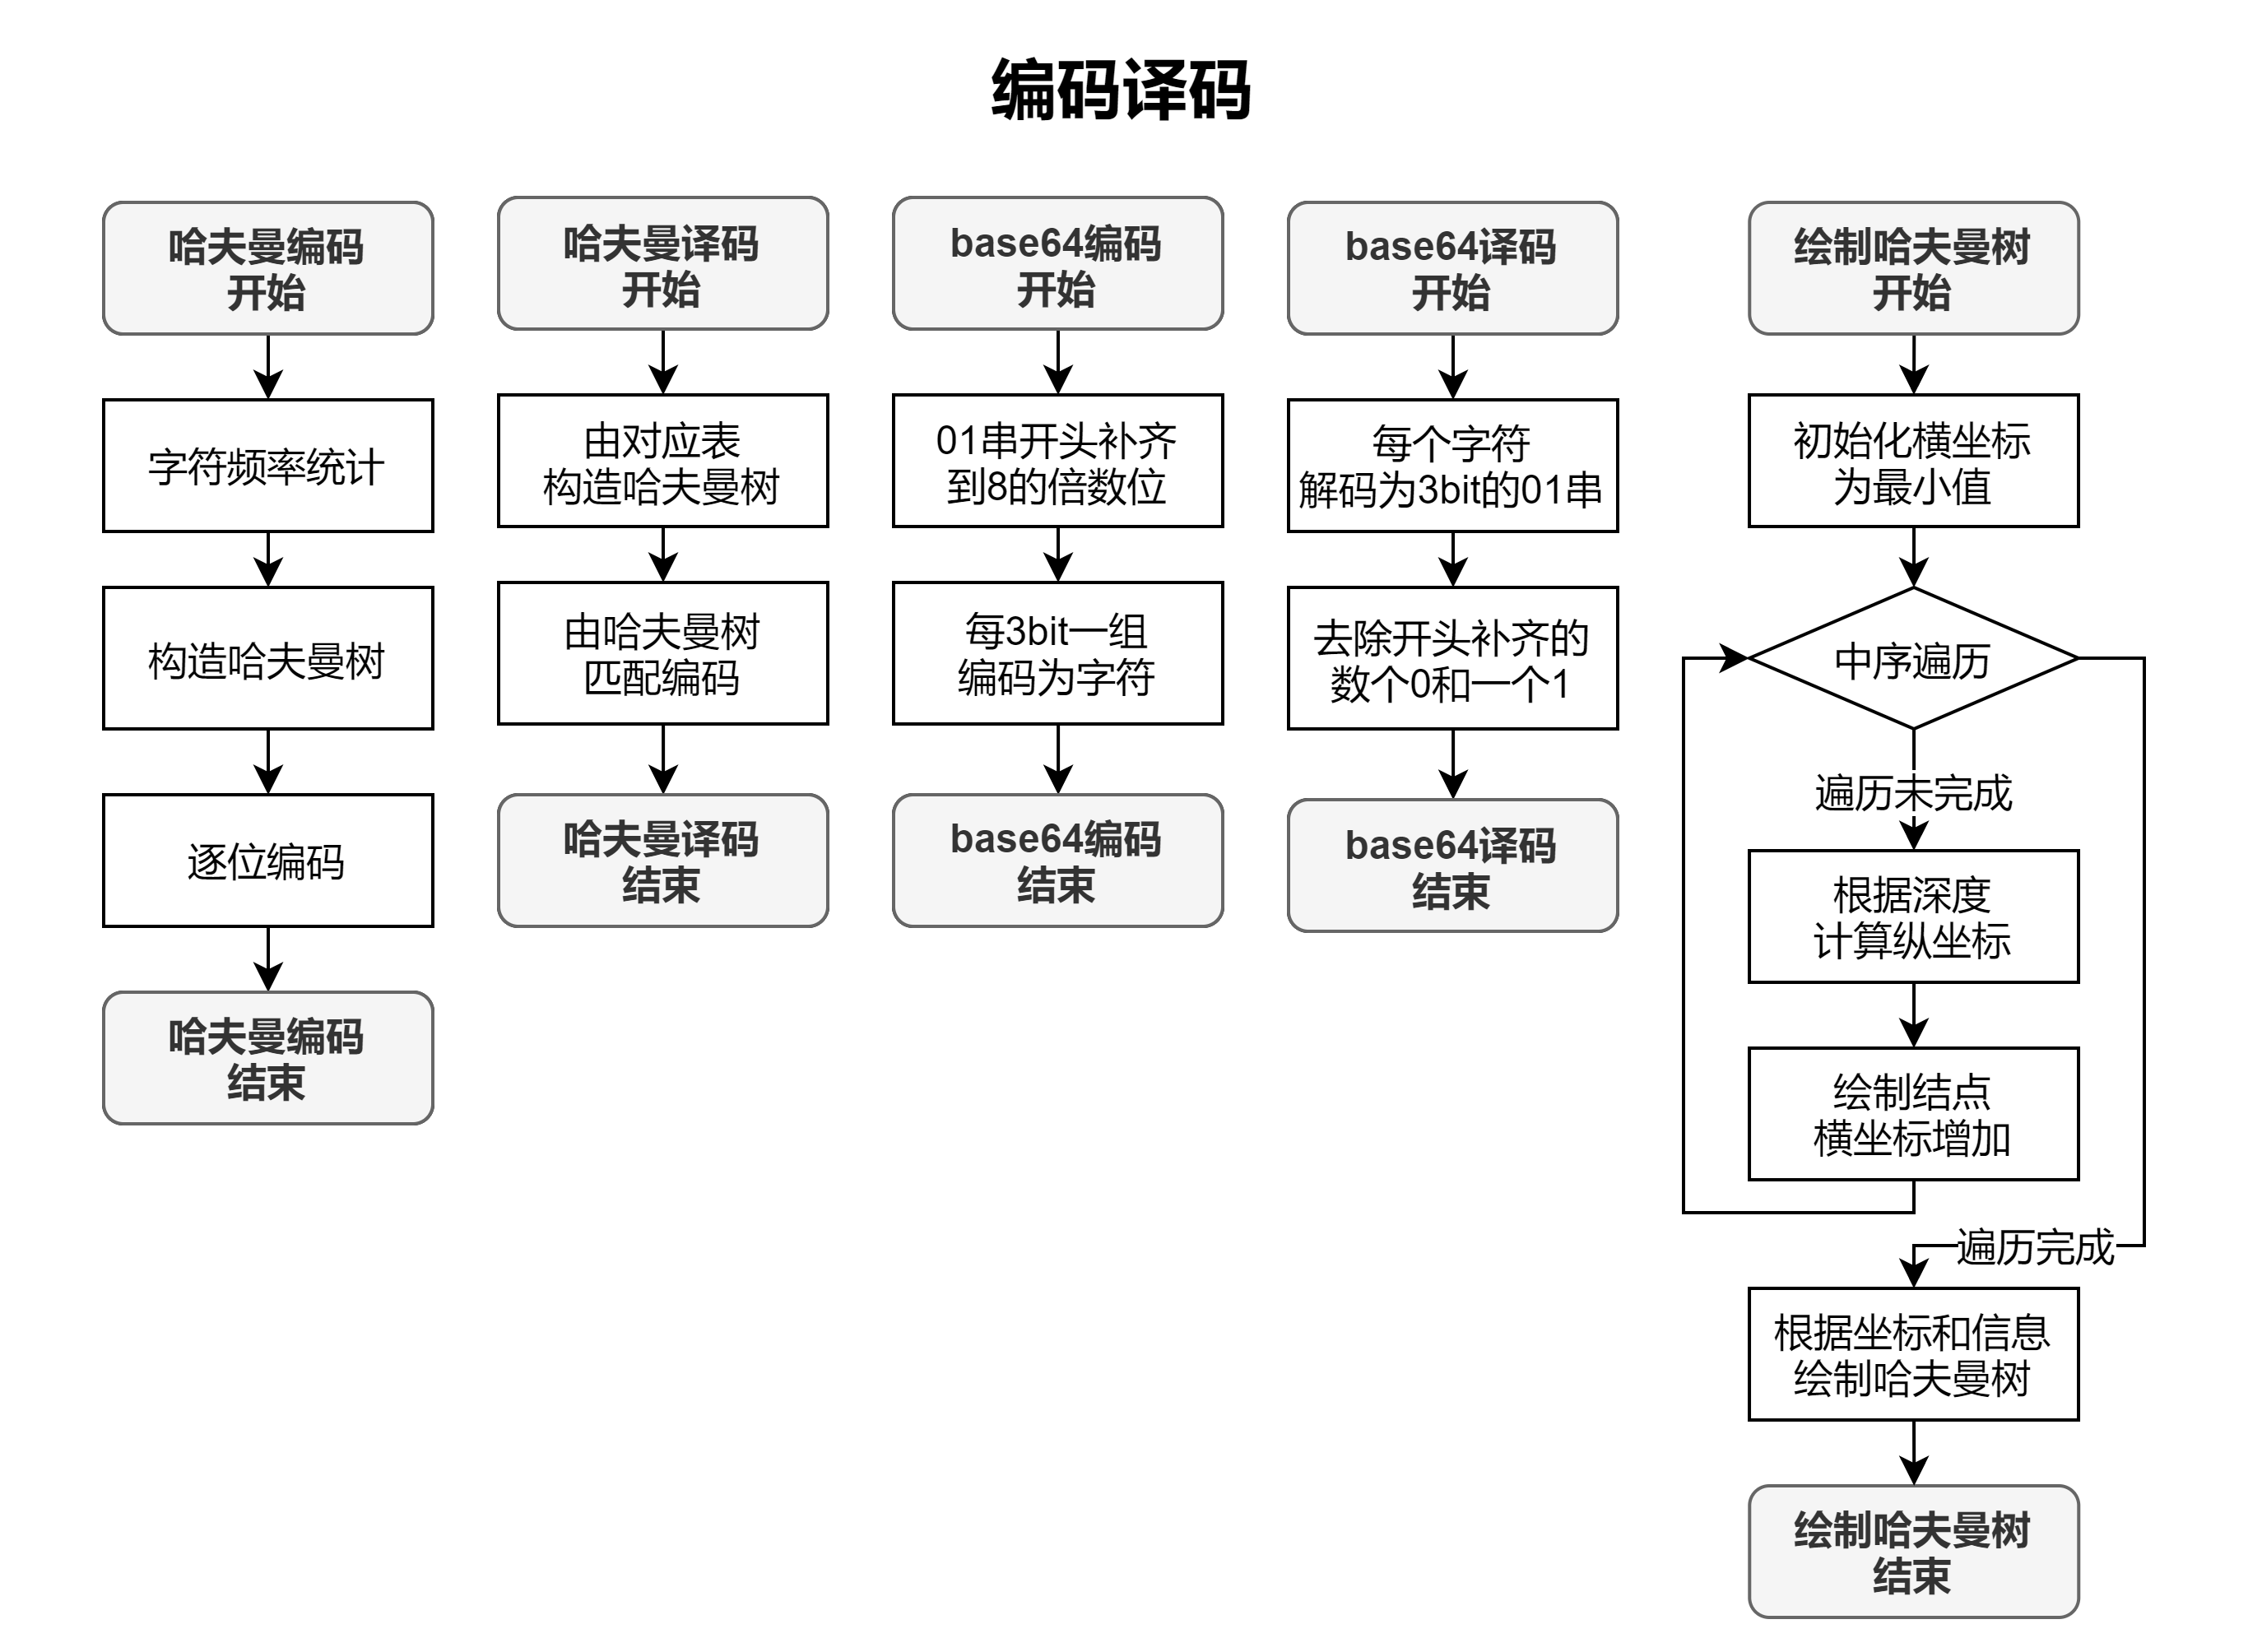
\includegraphics[width=\textwidth]{images/dsacd-流程图-编码译码.drawio.png}
    \caption{编码译码流程图}
\end{figure}

\begin{figure}[h]
    \centering
    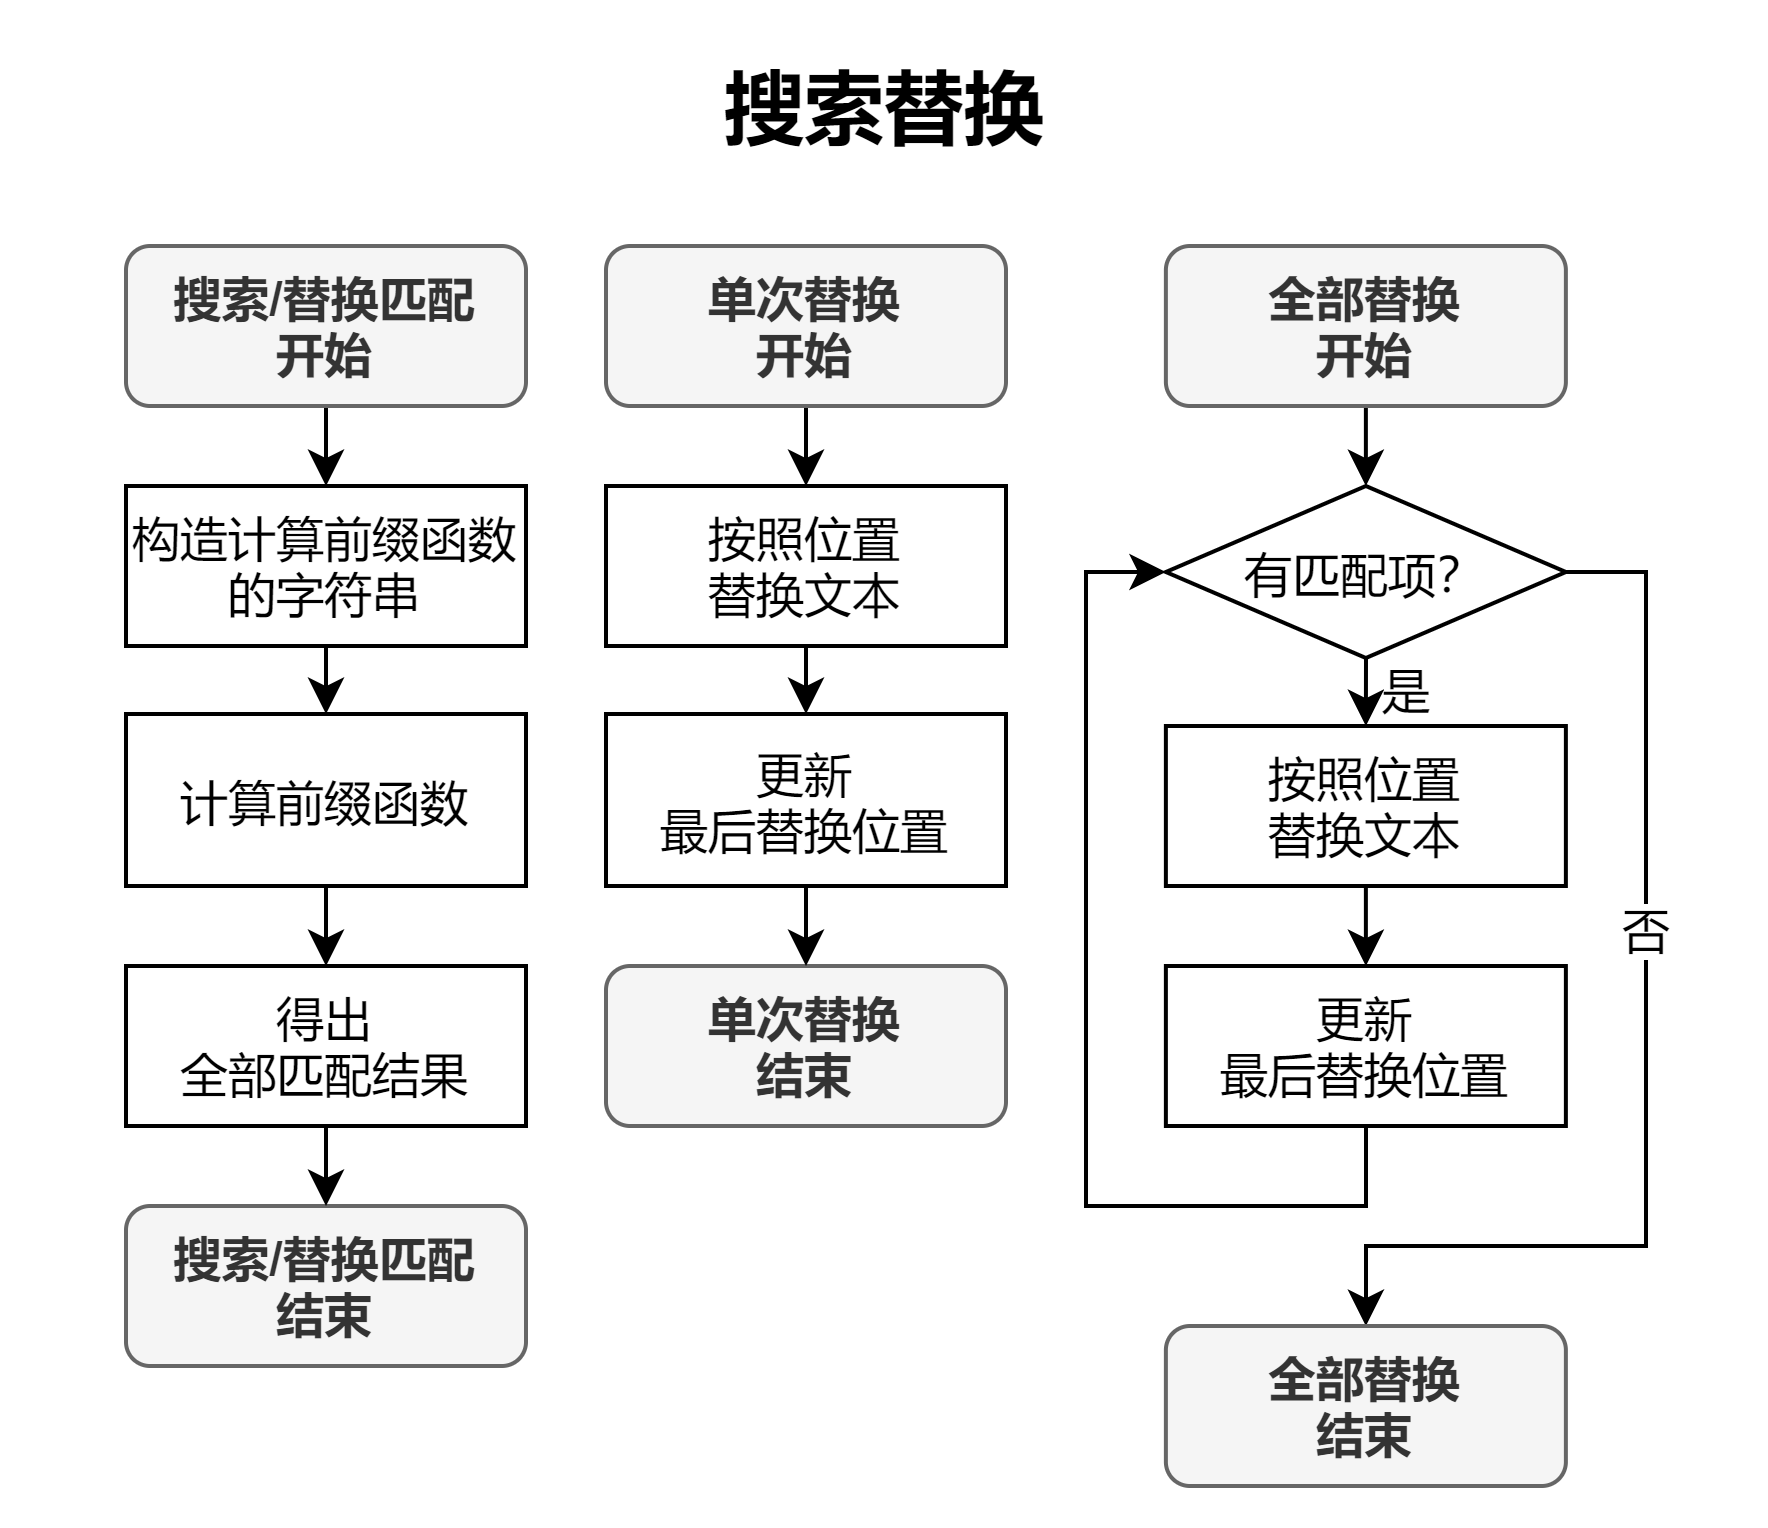
\includegraphics[width=0.6\textwidth]{images/dsacd-流程图-搜索替换.drawio.png}
    \caption{搜索替换流程图}
\end{figure}

\begin{figure}[h]
    \centering
    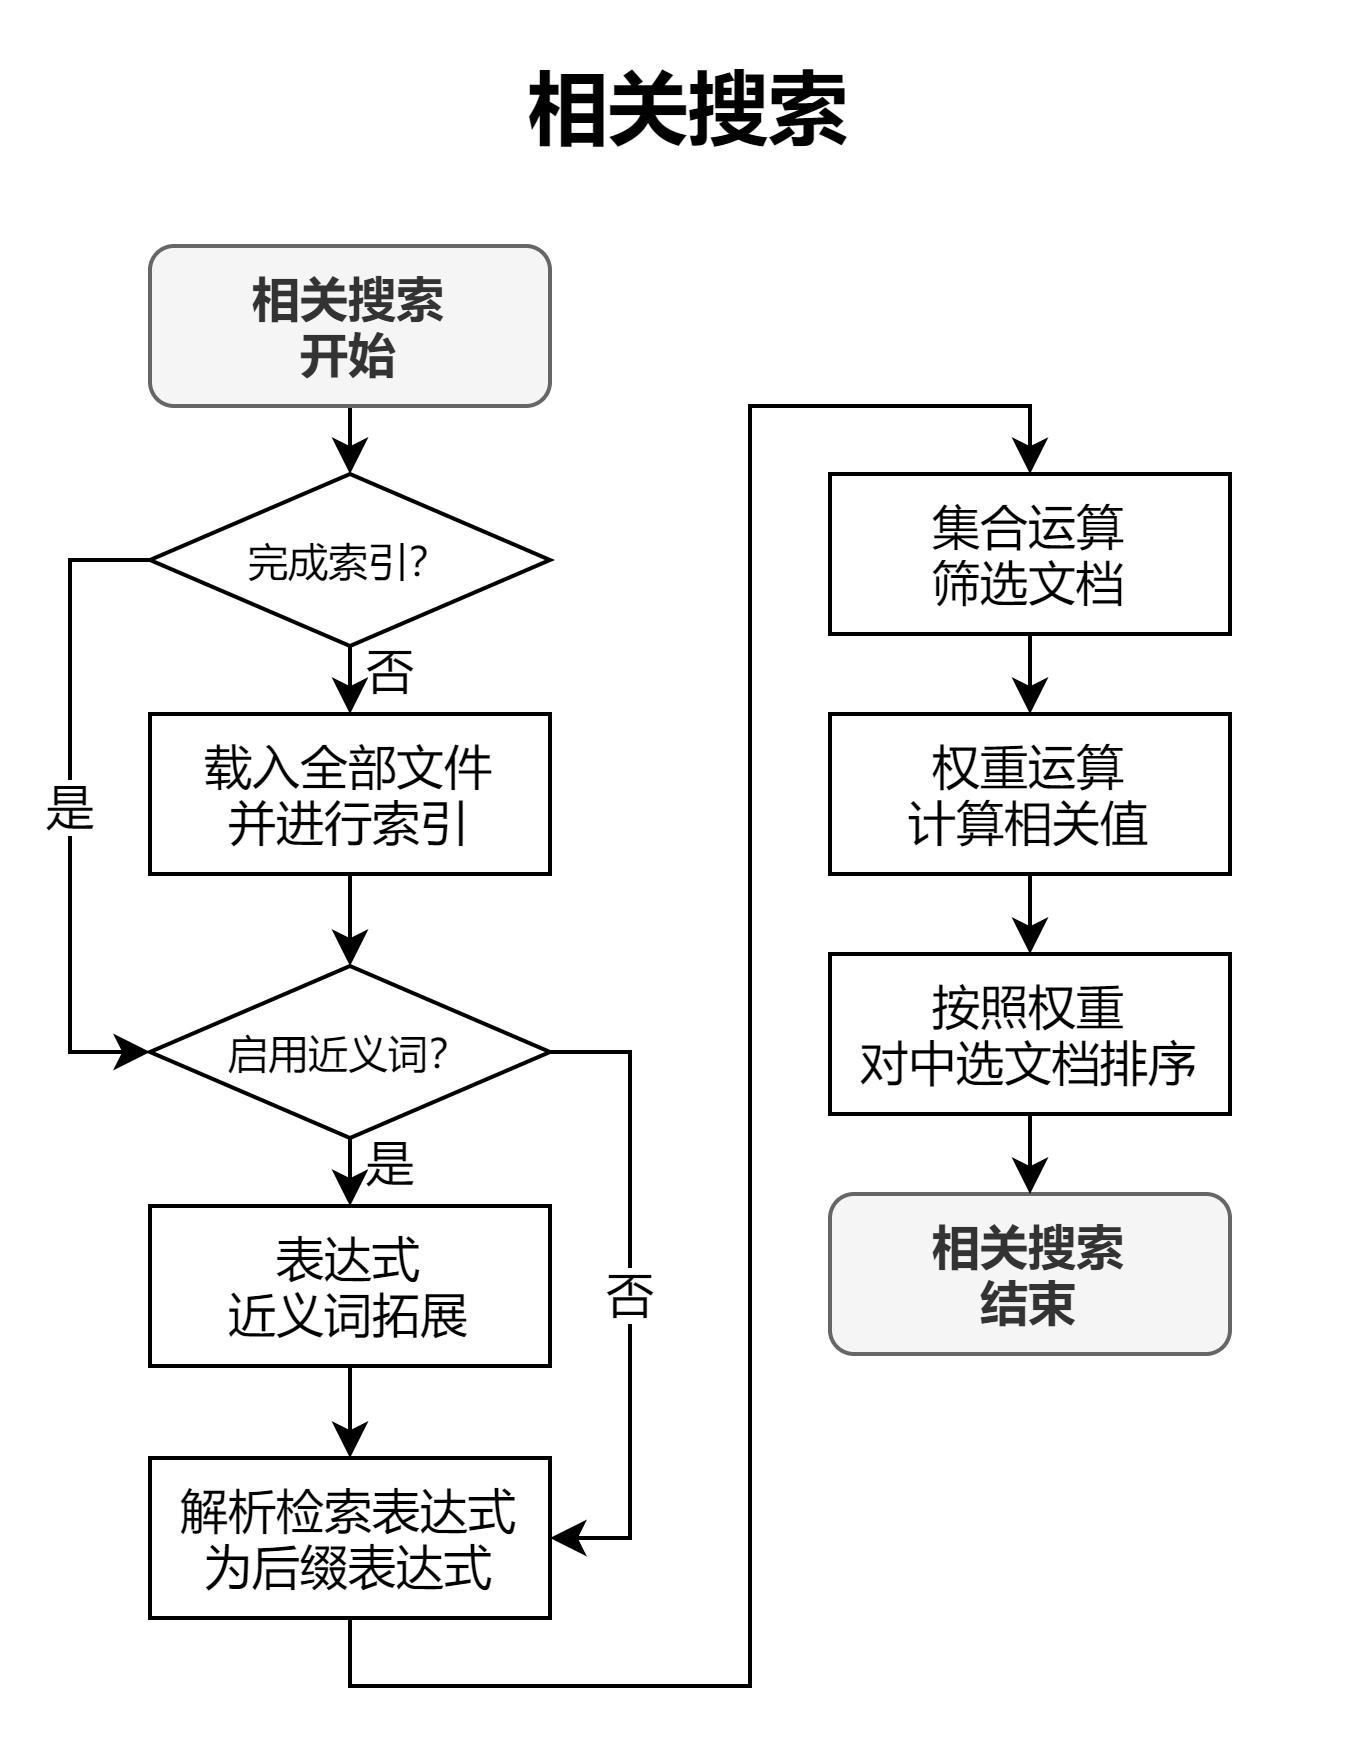
\includegraphics[width=0.6\textwidth]{images/dsacd-流程图-相关搜索.drawio.png}
    \caption{相关搜索流程图}
\end{figure}

\begin{figure}[h]
    \centering
    \begin{minipage}[t]{0.48\textwidth}
        \centering
        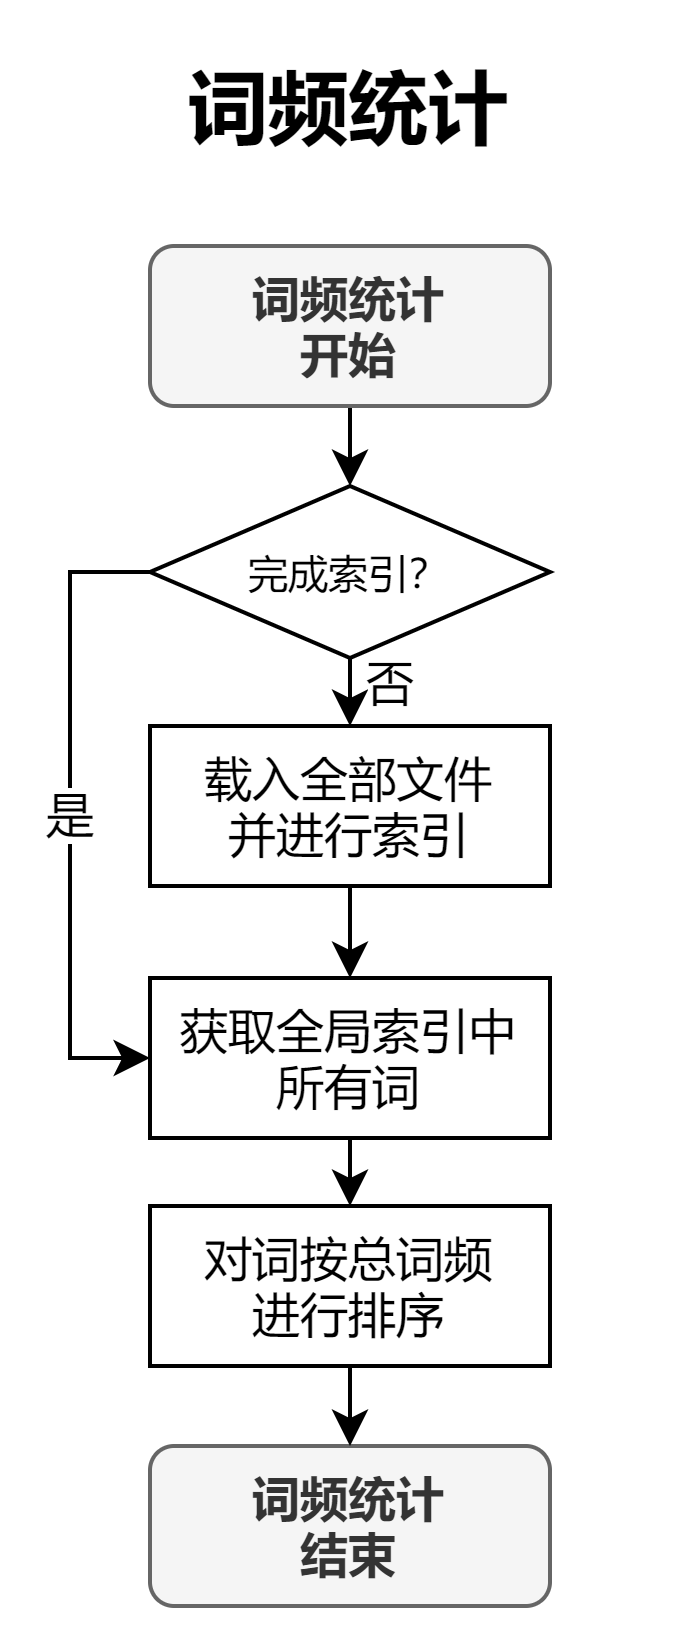
\includegraphics[width=0.6\textwidth]{images/dsacd-流程图-词频统计.drawio.png}
        \caption{词频统计流程图}
    \end{minipage}
    \begin{minipage}[t]{0.48\textwidth}
        \centering
        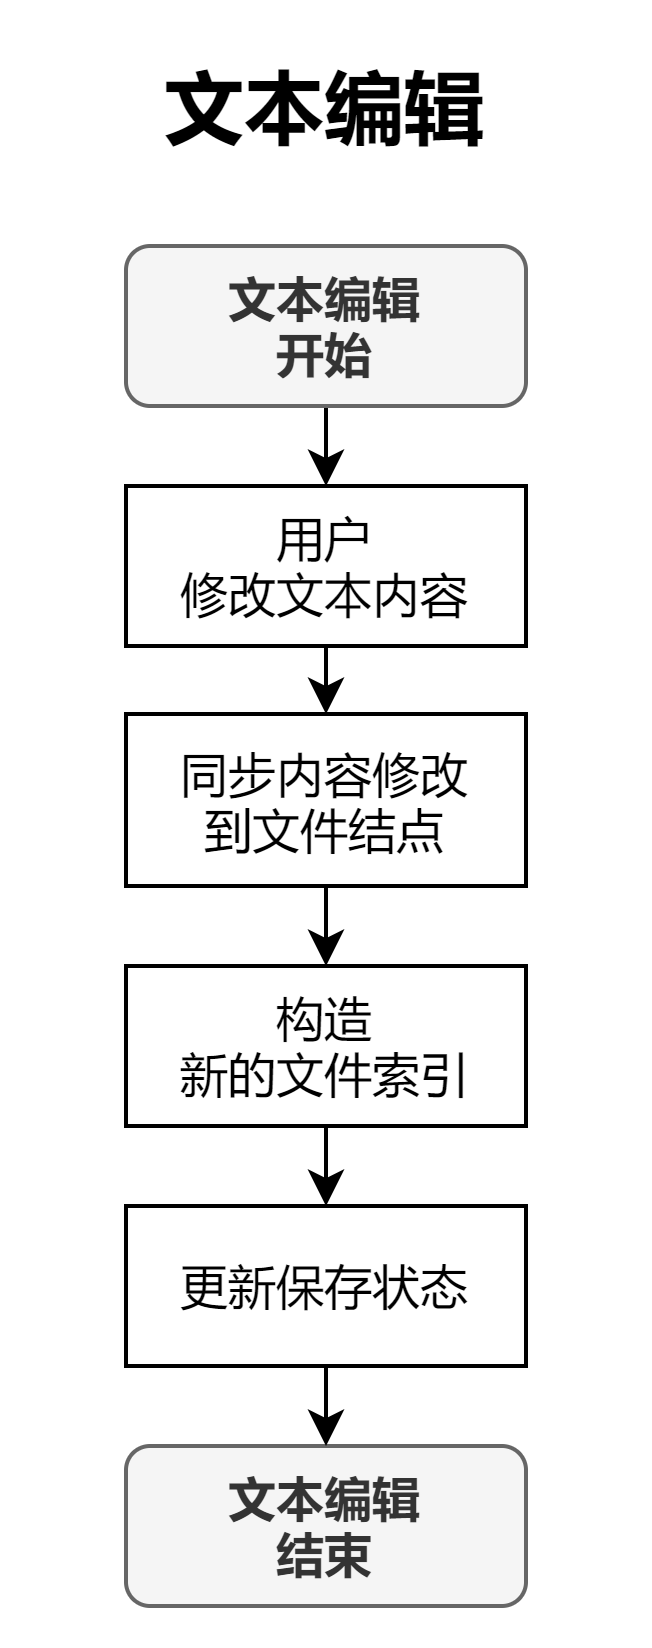
\includegraphics[width=0.6\textwidth]{images/dsacd-流程图-文本编辑.drawio.png}
        \caption{文本编辑流程图}
    \end{minipage}
\end{figure}

\subsubsection{各部分流程图}
各部分流程图包括开始部分、文件管理、编码译码、搜索替换、词频统计、相关搜索和文本编辑部分。

\clearpage

\section{测试}

\subsection{功能性测试}

\subsubsection{普通测试用例}
使用普通测试用例对各侧栏进行功能性测试,均工作正常。由于前面“系统整体结构以及各模块的功能描述”中详细描述了各模块的功能,这里不再赘述。

\begin{figure}[h]
    \centering
    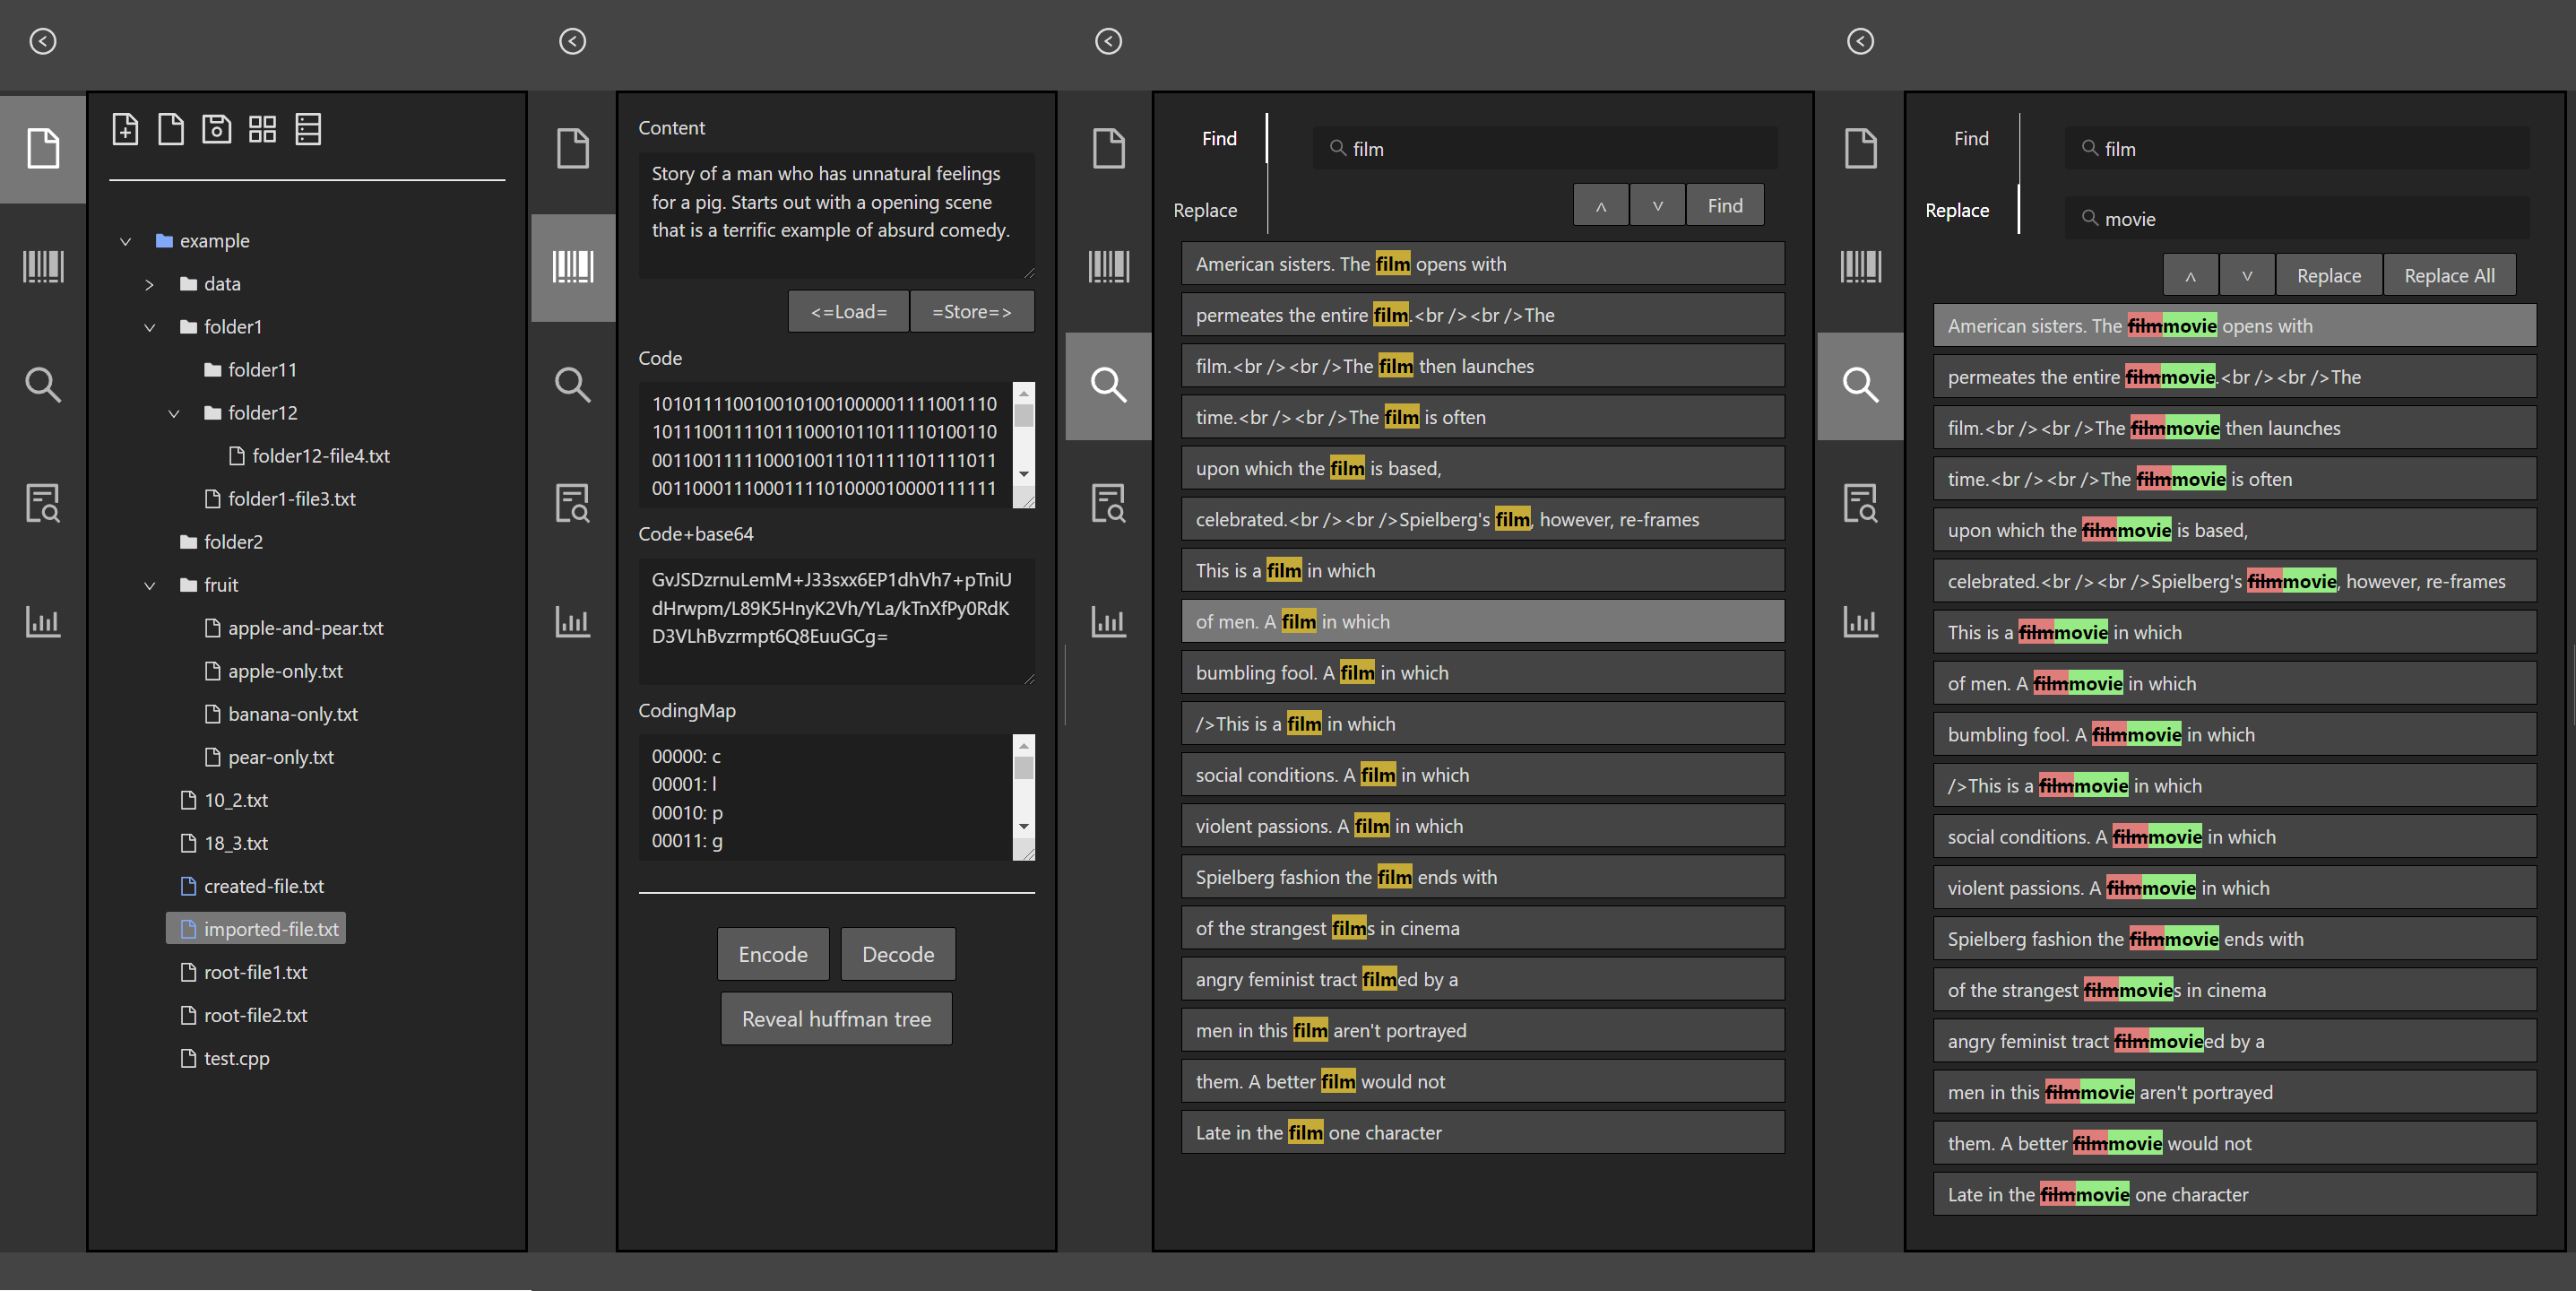
\includegraphics[width=\textwidth]{images/测试-1.png}
    \caption{前三个侧栏的测试截图}
\end{figure}

\begin{figure}[h]
    \centering
    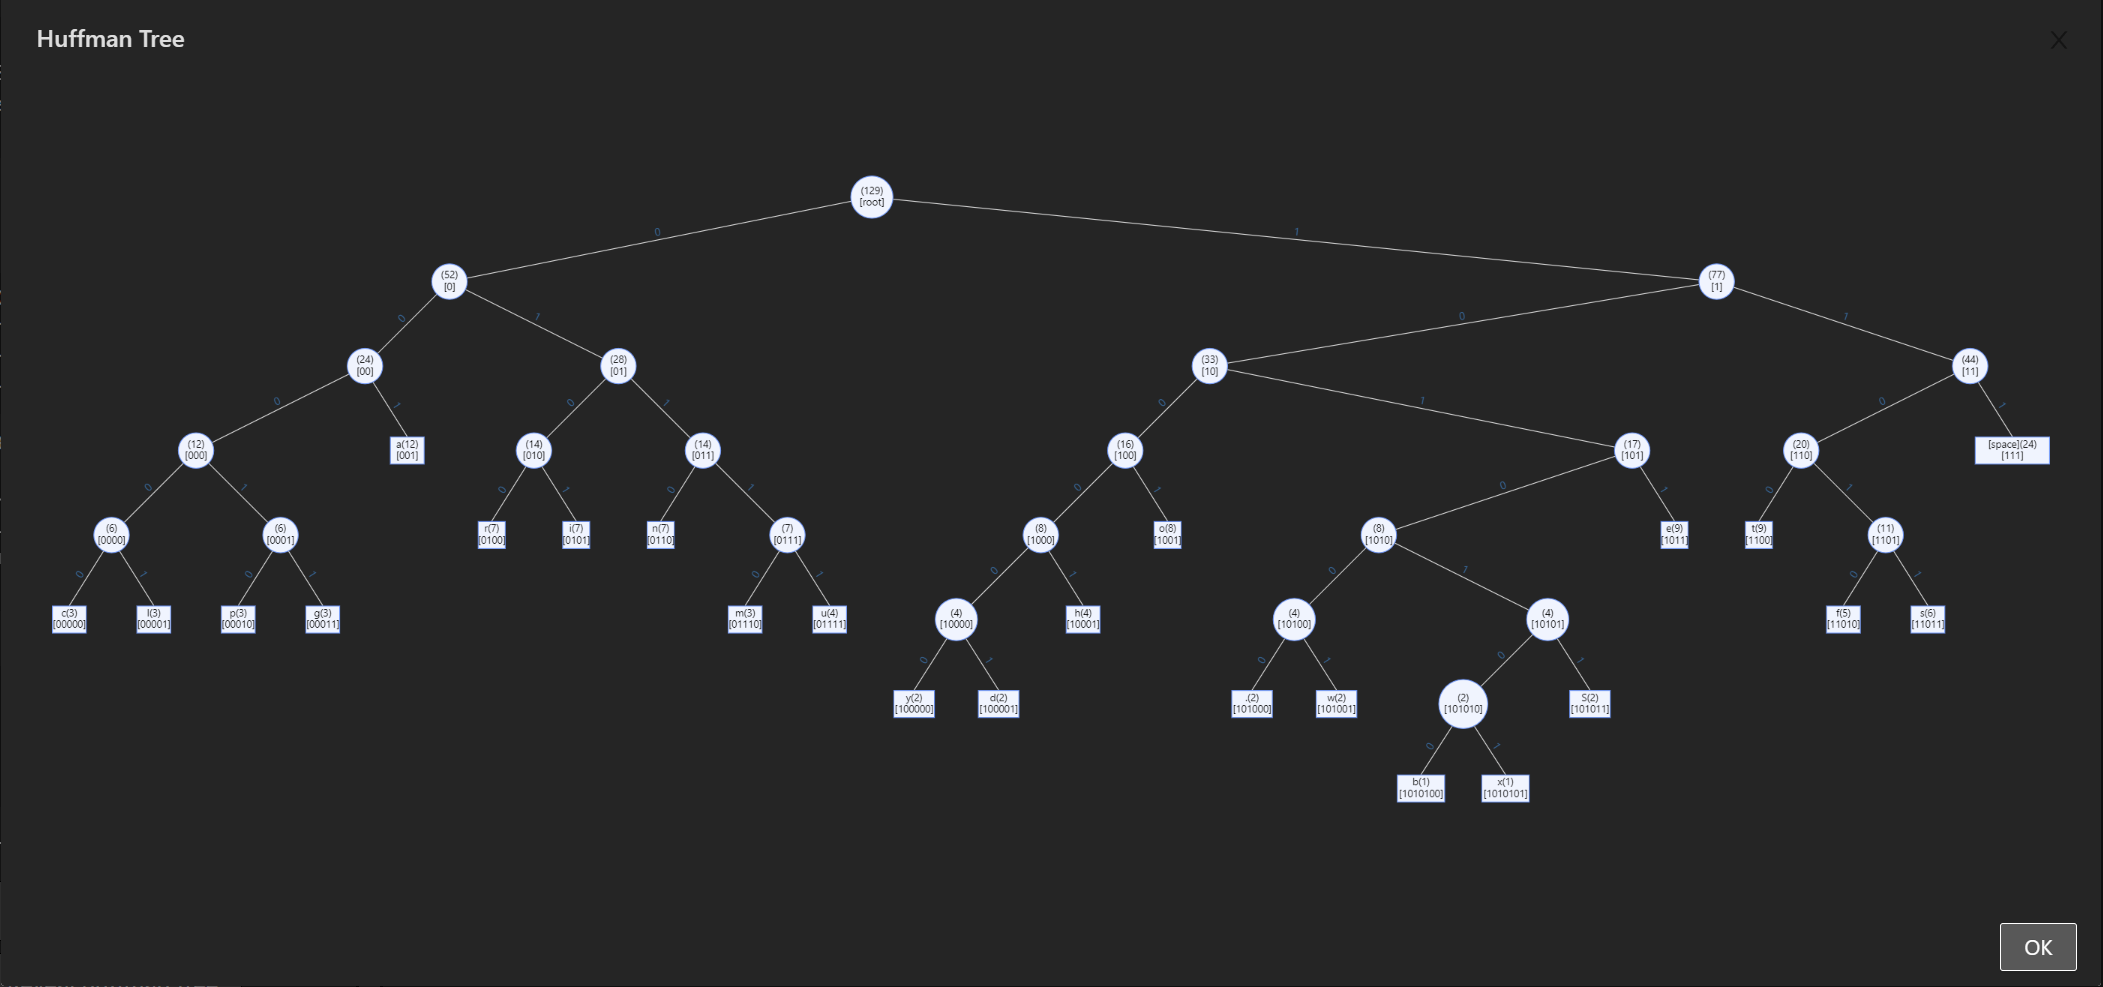
\includegraphics[width=0.8\textwidth]{images/测试-哈夫曼树.png}
    \caption{编码译码侧栏中展示的哈夫曼树}
\end{figure}

\begin{figure}[H]
    \centering
    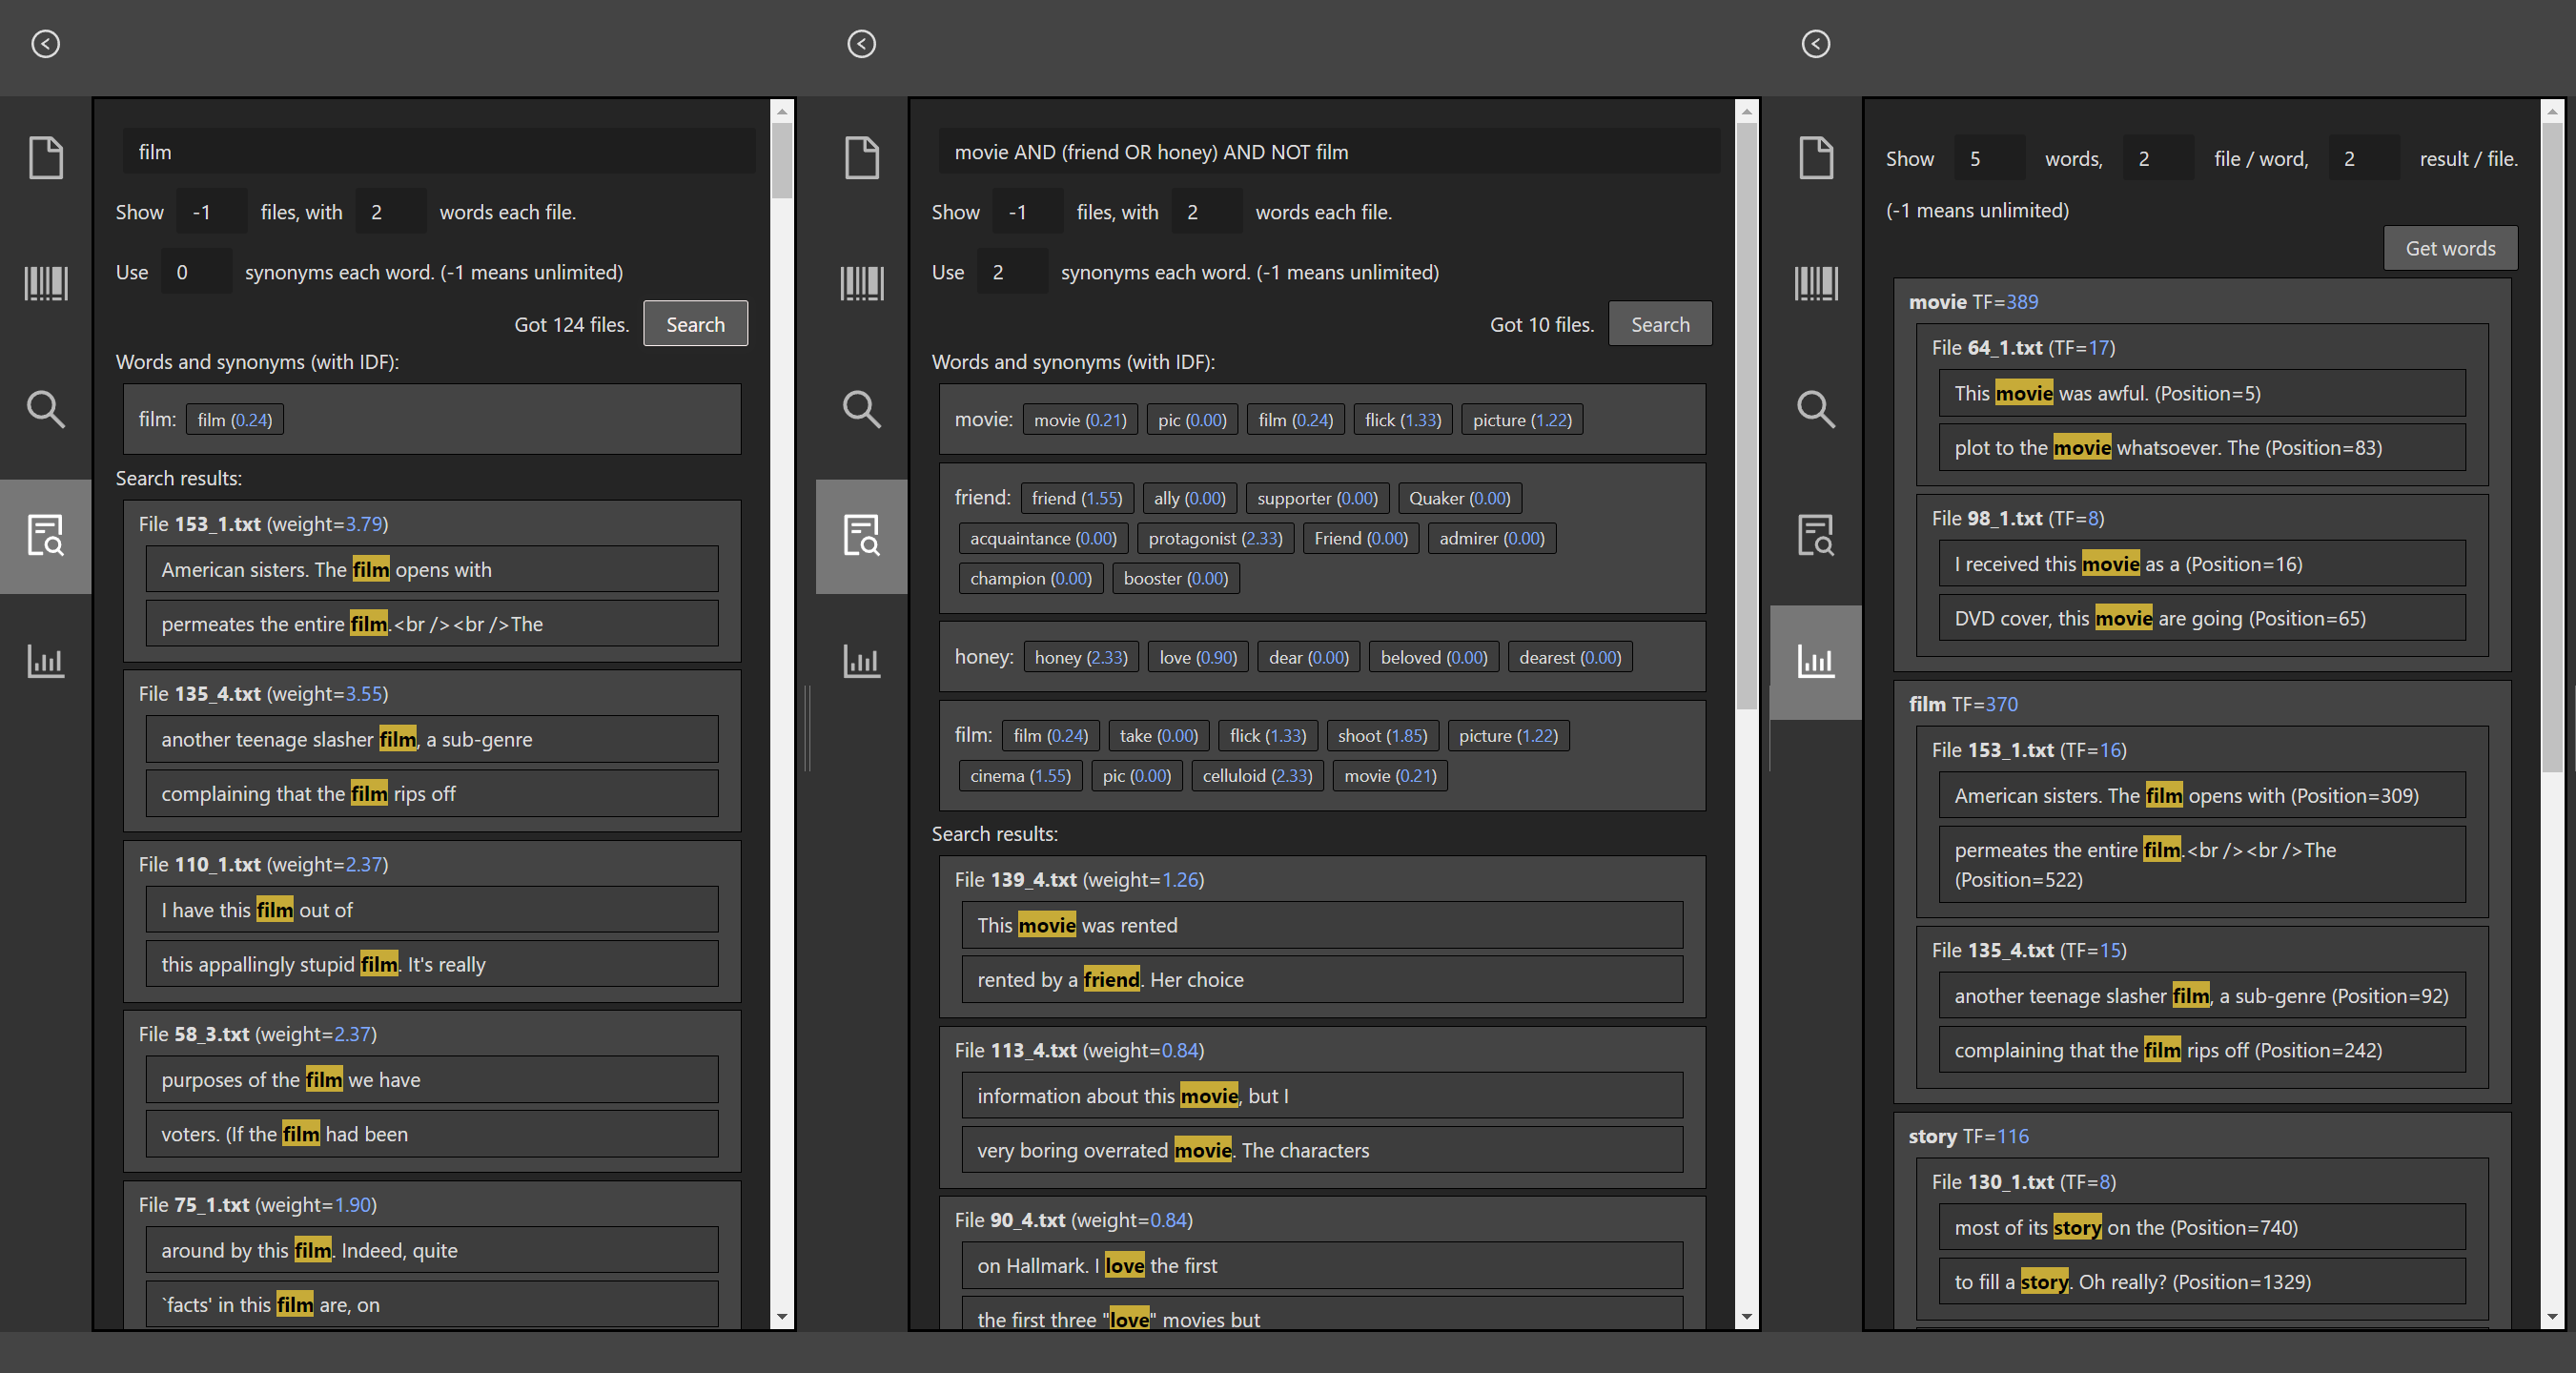
\includegraphics[width=\textwidth]{images/测试-2.png}
    \caption{后两个个侧栏的测试截图}
\end{figure}

\subsubsection{导致程序报错的用例}
此部分展示系统对特殊输入的报错和警告。

\paragraph{编码、搜索空内容报错}
在编码译码侧栏中,若用户尝试编码空内容,会在页面上方提示报错。同样地,在搜索替换侧栏中搜索空内容也会产生类似的报错。

\begin{figure}[H]
    \centering
    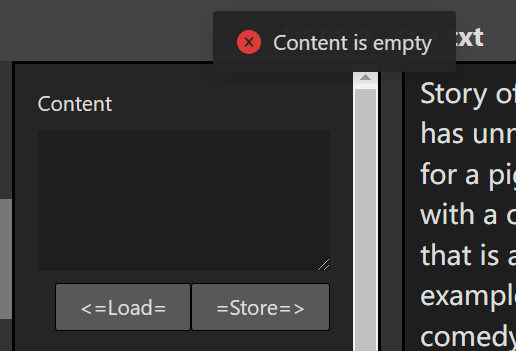
\includegraphics[width=0.4\textwidth]{images/问题-编码空内容报错.png} \\
    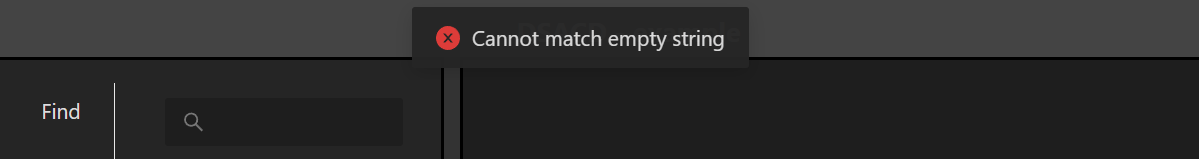
\includegraphics[width=0.8\textwidth]{images/问题-查找空内容.png}
    \caption{编码空内容报错}
\end{figure}

\paragraph{保存提醒}
在用户未对所有文件保存就要退出当前文件夹时,会弹出保存提醒框。用户可以选择保存所有文件、不保存,或者返回编辑界面继续修改。

\begin{figure}[H]
    \centering
    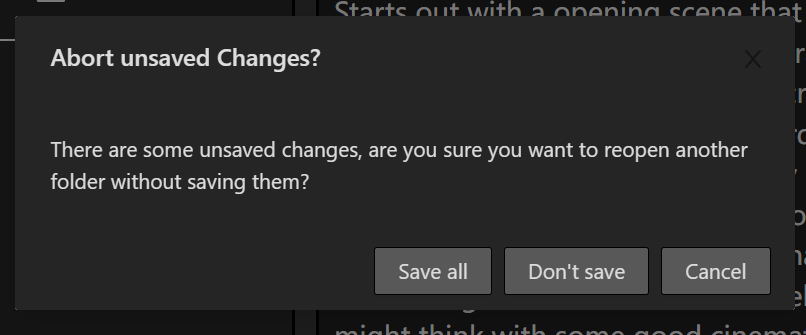
\includegraphics[width=0.6\textwidth]{images/问题-保存提醒.png}
    \caption{保存提醒}
\end{figure}

\paragraph{搜索无匹配}
当用户搜索的内容没有匹配项时,程序会在页面弹出警告,说明本次搜索未匹配任何内容。

\begin{figure}[H]
    \centering
    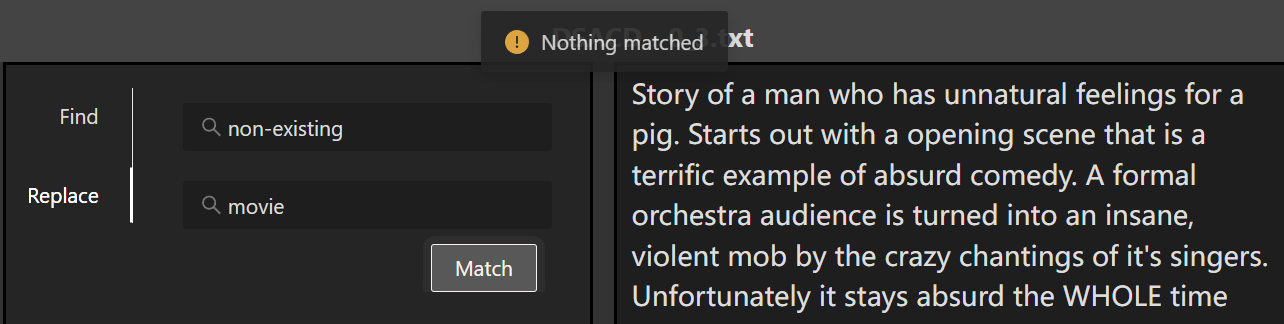
\includegraphics[width=0.8\textwidth]{images/问题-搜索无匹配.png}
    \caption{搜索无匹配}
\end{figure}

\subsubsection{边界数据测试}

\paragraph{相关性检索空文件夹}
我尝试让系统检索空文件夹,结果与预想的一致,没有任何检索结果。

\begin{figure}[H]
    \centering
    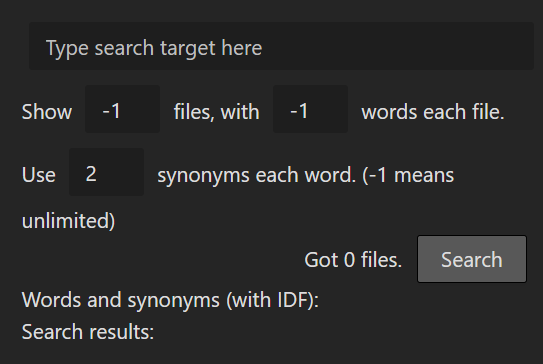
\includegraphics[width=0.8\textwidth]{images/测试-检索空文件夹.png}
    \caption{搜索无匹配}
\end{figure}

此外,许多边界测试,如搜索空内容、编码空内容,都在前面的部分进行了测试,系统会针对这些边界情况进行特殊的处理和报错。这些测试同样属于边界数据测试,但在此不再重复说明。

\clearpage

\subsection{非功能性测试}
测试对提高的文档进行索引,全部完成共耗时约5.6s。考虑到索引过程中也可以先对已完成索引部分先进行检索,程序运行效率可以接受。

此外,程序在载入和检索文件时,页面上方会弹出提示,向用户提示此过程的进行。

\begin{figure}[h]
    \centering
    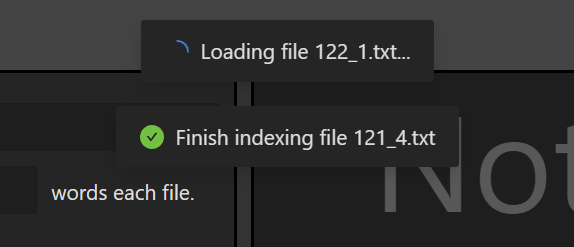
\includegraphics[width=0.4\textwidth]{images/测试-载入检索文件.png}
    \caption{载入检索文件}
\end{figure}

\clearpage

\section{总结与提高}

\subsection{亲手实现基础数据结构的经验}
在通常的开发过程中,亲自去实现基础数据结构是比较罕见的。在面向工程的场景下,我们通常可以使用可靠的标准库,还能使用充分验证、功能丰富的包;而在面向竞赛的场景下,我们几乎一定会使用STL等标准库以节约开发和运行的时间。

因此,亲手去开发如哈希表、对应表、堆等基础的数据结构是十分难得的。亲自实现这些基础数据结构让我对它们加深了理解,在将来的使用中也能更多地理解它们内部的原理,进而有助于进行调试、优化等工作。

\subsection{分层次、分模块地构建一个多功能程序}
之前在开发EduOJ等程序时,也脱离不开分层次、分模块地对程序进行构建,但此课设中,这一点体现得更加透彻。

\paragraph{层次} 课设分为三个层次,从低到高分别是:自己实现的基础数据结构与算法、面向应用的组合数据结构、业务逻辑与交互界面。

例如,对于相关性检索功能。最底层的是基础的中缀表达式转后缀、后缀表达式求值;中间的是面向相关性搜索构建的集合运算、权重运算;最上层的是与用户交互的界面、对检索结果的排序和分层次展示。

\paragraph{模块} 课设在图形化界面、数据结构上都分为了多个模块。图形化界面中每个Vue的Component就是一个模块,每种数据结构是一个模块。

\paragraph{“分治”的开发过程} 经过对一个大系统分层次、分模块的划分,我得以从低到高,逐个模块地对系统进行开发。每次开发一个层次中的一个模块,这有助于我全身心地思考模块的设计,也易于对各个模块进行测试。

\subsection{鸣谢}
在此,十分感谢本课设的指导老师,也是教授我们数据结构课设与算法的老师。

上学期的数据结构与算法课程中,杜老师对数据结构和算法的讲解十分清晰明了,本课设中大部分的数据结构均按照课堂讲授的思路实现。

此外,在课设教学中,杜老师从原型设计到验收检查都为我提供了明确的指导,对此课设有很大的帮助。

\end{document}